


%%%%%%%%%%%%%%%%%%%%%%%%%%%%%%%%%%%%%%%%%%%%%%%%%%%%%%%%%%%%%%%%%%%%%%%
%%%% Re-released for translation 22 June 2023  %%%%%%%%%%%%%%%%%%%%%%%%%%
%%%%%%%%%%%%%%%%%%%%%%%%%%%%%%%%%%%%%%%%%%%%%%%%%%%%%%%%%%%%%%%%%%%%%%%


\nbbbbbb{Endurants: Internal and Universal Domain Qualities}\label{chap4.tex.1}
\pos{\minitoc}{}

\vspace*{2mm}

\noindent
\begynd
\pind Please consider Fig.\,\vref{onto.fig2}.
\begynd
\pind The previous chapter covered the tree-like structure to the left in  Fig.\,\ref{onto.fig2}.
\pind This chapter covers the \ysf{vertical and  hori\ysfchg{z}ontal} lines, also
      to the left\ysf{,} in Fig.\,\ref{onto.fig2}.
\afslut
\afslut

\treprikker

\mnewfoil

\HHHH
\noindent 
\begynd
\pind In this chapter we introduce 
\begynd 
\pind the concepts of internal qualities of endurants and \ysf{some} universal
      qualities of domains, 
\pind and cover, first, the analysis and description of internal qualities:
\LLLL\HHHH
\begynd
\pind \bbcolor{unique identifiers} (Sect.\,\vref{chap4.Unique Identification}),
\pind \bbcolor{mereologies} (Sect.\,\vref{chap4.Mereology}) and
\pind \bbcolor{attributes} (Sect.\,\vref{chap4.Attributes})\ysf{.}
\afslut
\mnewfoil
\pind There is, additionally, three \sort{universal qualities:}
\begynd
\pind \bbcolor{space}, \bbcolor{time} (Sect.\,\vref{space and time}) and
\pind \bbcolor{intentionality} (Sect.\,\vref{chap4.Intentional Pull}), where
\begynd
\pind \sfsl{intentionality} is  ``something'' that expresses
\pind intention, design idea, purpose of artefacts -- 
\pind well, some would say, also of natural endurants.
\afslut
\afslut
\afslut

\mnewfoil

\pind As it turns out\pos{\footnote{You, the first time reader cannot
    know this, i.e., the ``turns out''. Once we have developed and
    presented the material of this chapter, then you can see it;
    clearly\,!}}{\stepcounter{footnote}}, 
\begynd
\pind to analyse and describe mereology
\pind we need to first analyse and describe unique identifiers;
\afslut
and
\begynd
\pind to analyse and describe attributes
\pind we need to first analyse and describe mereologies.
\afslut
\mnewfoil
\pind Hence:
\afslut

\procmeth{\nyl{Sequential Analysis \& Description of} \nyl Internal
          Qualities}{methstp:saadoiq}{%
\begynd
\pind We advise that the \ysf{domain modeller:}
\begin{itemize}
\item  \sort{first} analyse \& describe  \nyl \bbcolor{unique identification} of all endurant sorts;
\item  \sort{then}  analyse \& describe \nyl \bbcolor{mereologies} of all endurant sorts;
\item  \ysf{\sort{then}} analyse \& describe \nyl \bbcolor{attributes}
  of all endurant sorts; and,
\item  \ysf{\sort{finally}, to analyse \& describe \nyl \bbcolor{intentionality}.} 
\end{itemize}
\afslut}

\bookdefn{Description, II}{ %
\begynd
\pind By a \sort{description} \index{pdefind}{description!internal qualities} of the internal
      qualities of a domain
\begynd
\pind we mean pairs of informal, narrative, and formal text
\pind which characterises the
\begynd
\pind unique identifiers,
\pind mereologies,
\pind attributes, and possible
\pind intentional pulls
\afslut
\pind of manifest parts (fluids and living species) \dbsquare
\afslut
\afslut
}

\noindent
\begynd
\pind This chapter explains what is meant by 
\begynd
\pind \sfsl{unique identifier}, \index{pconind}{unique identifier} 
\pind \sfsl{mereology},  \index{pconind}{mereology}
\pind \sfsl{attribute} and \index{pconind}{attribute}
\pind \sfsl{intentional pull}. \index{pconind}{intentional pull}
\afslut
\afslut
\mnewfoil

\nbbbbb{Internal Qualities}\label{chap4.Internal Qualities}

\noindent
\inthis{\nyl internal qualities}{the properties
of the entities \nyl to which we ascribe internal qualities.}{}

\nbbbb{General Characterisation}

\begynd%
\pind {External qualities} of endurants of a manifest domain
\begynd
\pind are, in a simplifying sense, those we can
\begynd
\pind see and
\pind touch.
\afslut
\pind They, so to speak, take form.
\afslut
\afslut
\pos{\psno}{\mnewfoil}%

\begynd%
\pind \bbcolor{Internal qualities} of endurants of a manifest domain
\begynd
\pind are, in a less simplifying sense, those which
\begynd
\pind we may not be able to see or ``feel'' \nyl when touching an endurant,
\pind but they can, as we now `mandate' them,
\begynd
\pind be reasoned about, \nyl as for \brcolor{unique identifiers} \nyl and \brcolor{mereologies},
\afslut or
\pind be measured by some \sort{physical/chemical} means,
\pind or be ``spoken of'' by \sort{intentional deduction}, and
\begynd
\pind be reasoned about,
\afslut
\pind as we do when we \brcolor{attribute} properties to endurants.
\afslut
\afslut
\afslut

\nbbbb{Manifest Parts versus Structures}

\begynd
\pind In \cite{BjornerMonograph2020} we covered a notion of \sfsl{`structures'}.
\begynd
\pind In this primer we shall treat \nyl  the concept of `structures'
differently\ysfchg{. }
\pind We do so by distinguishing between
\begynd
\pind manifest parts 
\pind and structures.
\afslut
\afslut
\afslut

\nbbb{Definitions}

\bookdefn{Manifest Part:}{ By a manifest part\index{pdefind}{manifest
      part}\index{pdefind}{part!manifest} we shall understand
\begynd
\pind a part which `manifests' itself 
\begynd
\pind either in a physical, visible
      manner, ``occupying'' \nyl an $\mathbb{AREA}$ or \nyl a $\mathbb{VOLUME}$
      and \nyl a $\mathbb{POSITION}$  \nyl in  $\mathbb{SPACE}$, 
\pind or in a conceptual manner \nyl  forms an organisation in Your
      mind\,!\dbsquare\ \
\afslut 
\pind As we have already revealed,   
\pind endurant parts can be \nyl transcendentally
      deduced into perdurant behaviours   
\pind -- with manifest parts indeed being so.
\afslut}

\mnewfoil
\bookdefn{Structure}{ By a structure\index{pdefind}{structure} we shall
      understand
\begynd
\pind an endurant concept that allows \nyl  the domain \ysf{modeller}
\begynd
\pind to rationally decompose \nyl  a domain analysis and/or its description 
\pind into manageable, logically relevant sections,  
\pind but where these abstract endurants \nyl  are not further reflected
      upon \nyl  in the domain analysis and description.
\afslut
\pind Structures are therefore \nyl  not  transcendentally
      deduced into perdurant behaviours.
\afslut}

\nbbb{Analysis Predicates}

\daprompt{is\_manifest}{is-manifest}{\label{is manifest pt}%
\begynd
\pind The method provides the \dap:
\begin{itemize}
\item \bcolor{\texttt{is\_manifest}}
     \doanpr\pos{\apindex{is\_manifest}}{}
      -- where 
      \texttt{is\_manifest($p$)} \nyl  holds if $p$ is to be considered manifest\eoap
\end{itemize}
\afslut
}
\daprompt{is\_structure}{is-structure}{\label{is structure pt}%
\begynd
\pind The method provides the \dap:
\begin{itemize}
\item \bcolor{\texttt{is\_structure}}
     \doanpr\apindex{is\_structure}
      -- where 
      \texttt{is\_structure($p$)} \nyl  holds if $p$ is to be considered a structure\eoap
\end{itemize}
\afslut
}

\noindent
\begynd
\pind The obvious holds:
      \bcolor{\texttt{is\_manifest}(p)}\,{\IS}\,\ysfchgii{\SIM}\,\bcolor{\texttt{is\_structure}(p)}. 
\afslut

\nbbb{Examples}\LLLL
\monoexample{Manifest Parts and Structures}{\LLLL
  We refer to Example\,\vref{A Road Transport System Domain: Cartesians}: the Road
     Transport System.
\begynd
\pind We shall consider all atomic parts: hubs, links and automobiles
      as being manifest. \nyl (They are physical, visible and in $\mathbb{SPACE}$.)
\pind We shall consider road nets and aggregates of automobiles as
      being manifest.
\begynd 
\pind Road nets are physical, visible and in $\mathbb{SPACE}$.
\pind Aggregates of automobiles are here considered conceptual.
\pind The road net manifest part, 
\begynd 
\pind apart from it\ysf{s} aggregates of hubs and links, 
\pind can be thought of as ``representing'' a \sfsl{Department of Roads}\footnotemark.
\afslut 
\pind The automobile aggregate 
\begynd
\pind apart from its automobiles,
\pind can be thought of as ``representing'' a \sfsl{Department of Vehicles}\footnotemark.
\afslut
\pind We shall\ysf{, at present,} consider hub and link aggregates and
hub and link set\ysf{s} as structures \eod
\afslut
\afslut}
\addtocounter{footnote}{-1}
\footnotetext{\LLLL -- of some country, state, province, city or other.}
\addtocounter{footnote}{1}
\footnotetext{\LLLL See above footnote.}

\nbbb{Modelling Consequence}\HHHH

\begynd
\pind \ysf{} If a part is considered manifest \nyl then we shall endow that part \nyl with all
      three kinds of internal qualities.
\pind If a part is considered a structure \nyl then we shall \sort{not}
      endow that part \nyl with any 
      of \ysfchg{the } three kinds of internal qualities.
\afslut

\nbbbbb{Unique Identification}\label{chap4.Unique Identification}

\noindent
\begynd
\pind The concept of parts having unique identifiability,
\begynd
\pind that is, that two parts, 
\pind if they are the same,
\pind have the same unique identifier,
\pind and if they are not the same,
\pind then they have distinct identifiers,
\pind that concept is fundamental to our being able \nyl
      to analyse and describe internal qualities of endurants.
\afslut
\pind So we are left with the issue of `identity'\,!
\pos{\pind \ysf{(We refer to Sect.\,\vref{IdentityKS}.)}}{}
\afslut

\mnewfoil

\bookdefn{Uniqueness}{ %
\begynd
\pind By uniqueness of parts we shall mean
\begynd
\pind that any two spatially distinct parts
\pind are two unique parts --
\pind cannot be confused \dbsquare\
\afslut
\afslut
}

\bookdefn{Unique Identifier}{ %
\begynd
\pind By a unique identifier we shall mean
\begynd
\pind anything that can be used to distinguish
\pind any one part from any other spatially distinct parts \dbsquare\
\afslut
\afslut
}

\nbbbb{On Uniqueness of Endurants}

\begynd
\pind We therefore introduce the notion of \nyl unique identification of
      part endurants.
\pind We assume
\begynd
\pind (i) that all part endurants, \textsf{e}, of any domain
      \textsf{E}, \nyl have 
      \pcindextermii{unique}{identifier}s, 
\pind (ii) that \pcindextermii{unique}{identifier}s
      (of part endurants \textsf{e:E}) \nyl 
      are \pcindextermii{abstract}{value}s \nyl
      (of the \pcindextermii{unique}{identifier} sort \textsf{UI} of part endurants
      \textsf{e:E}), 
\pind (iii) \ysf{} that distinct part endurant sorts, \textsf{E$_i$} and
      \textsf{E$_j$},\nyl\ have distinctly named
      \pcindextermii{unique}{identifier} sorts, \nyl say \textsf{UI$_i$} and
      \textsf{UI$_j$}\footnote{\LLLL This restriction is not
        necessary, but, for the time \ysfchg{being}, we can assume that it is.}, and 
\pind (iv) that all \textsf{$ui_i$:UI$_i$} and \textsf{$ui_j$:UI$_j$} are
      distinct.
\afslut
\afslut

\pos{\psno}{\mnewfoil}
\typo{\begynd
\pind The names of unique identifier sorts, say \textsf{UI}, \nyl is
      entirely at the discretion of \nyl  the \sfsl{domain \ysf{modeller}}.
      \pind If, for example, the sort name of a part\ \ is \textsf{P}, \nyl
     then it might be expedient to \nyl  name the sort of the unique
     identifiers of its parts \textsf{PI}.
\afslut}

\pos{\psno}{\mnewfoil}

\bgcolor{Representation of Unique Identifiers:}{ %
\begynd
\pind Unique identifiers are abstractions.
\begynd
\pind When we endow two endurants (say of the same sort) \nyl 
      distinct unique identifiers
\pind then we are simply saying that \nyl  these two endurants are distinct.
\pind We are not assuming anything about \nyl how these identifiers
      otherwise come about. 
\afslut%
\afslut%
}
\mnewfoil 
\bgcolor{Identifiability of Endurants:}{
\begynd
\pind From a philosophical point of view, 
\begynd
\pind and with basis in \kaisorfil\pos{, \nyl cf.\,Paragraph \bmcolor{Identity, Difference and
      Relations} (\pos{Page}{Slide}\,\pageref{Identity and Relations})}{}, 
\pind one can rationally argue that there are many endurants,
\pind and that they are unique, and hence uniquely identifiable.
\afslut
\pind From an empirical point of view,
\begynd
\pind and since one may eventually \nyl
      have a software development in mind,
\pind we may wonder how unique identifiablity can be accommodated.
\afslut
\afslut
}

\mnewfoil\HHHH
\begynd
\pind Unique identifiability for solid endurants,
\begynd
\pind even though they may be mobile, 
\pind is straightforward:
\begynd
\pind one can think of many ways  
\pind of ascribing a unique identifier to any part\ysf{.}
\afslut
\afslut
\pind Hence one can think of many such unique identification schemas.
\afslut

\mnewfoil
\begynd
\pind Unique identifiability for fluids may seem a bit more tricky.
\begynd
\pind For this \monograph\ we shall not suggest
\pind to endow fluids with unique identification.
\pind We have simply not experimented with such \nyl
      part-fluids and fluid-parts domains \nyl
      -- not enough -- to suggest so. 
\afslut
\afslut

\nbbbb{Uniqueness Modelling Tools}\label{kap4.Uniqueness Modeling Tools}
 
\begynd
\pind The analysis method offers an
      observer function \textsf{{\uidmo}E} \nyl which when applied to \ysfchg{a }
      part endurant\ysfchg{, } \textsf{e} \ysf{of sort \textsf{E}}, \nyl
      yields the unique identifier,  $ui$:\textsf{EI}, of \textsf{e}.
\afslut
\ddprompt{describe\_unique\_identifier}{observe-unique-identifier}{\label{duid}%%
\begynd
\pind We can therefore apply the \ddp:
\begin{itemize}
\item \bcolor{\texttt{describe\_unique\_identifier}}%
      \dodepr\dpindex{describe\_unique\_identifier}%% 
\end{itemize}
\emmar
\noindent
\pind to endurants \textsf{e:E} 
\begynd
\pind resulting in the analyser writing down
\pind the \ddtu{Unique Identifier Type and Observer} 
\afslut
\afslut
\mnewfoil\bdbrule

{\bgcolor{\bgcolor{\cdlti}\ 
      \texttt{describe\_unique\_identifier(e)}} \sort{Observer}}
      \delati{describe\_unique\_identifier}%
      \ddlt{PartUniqueIdentifier}{dlti}
%\RSLatex
%&\bq\kw{Narration:}&
%   [s]   ... narrative text on unique identifier sort EI ...&\footnotemark&
%   [u]   ... narrative text on unique identifier observer &{\uidmo}&E ...
%   [a]   ... &axiom on& uniqueness &of& unique identifiers ...
%& \kw{Formalisation:}&
%   type
%   [s]   UI
%   value
%   [u]   &{\uidmo}&E: E -> EI&\delaoi{\protect{\uidmo}}\label{uidP}\eq& 
%\endRSLatex 
\bp
\bq\kw{Narration:}\\
\>\ {\LBRACKET}s{\RBRACKET}\ \ \ {\DOTDOTDOT} narrative text on unique identifier sort EI {\DOTDOTDOT}\footnotemark\\
\>\ {\LBRACKET}u{\RBRACKET}\ \ \ {\DOTDOTDOT} narrative text on unique identifier observer {\uidmo}E {\DOTDOTDOT}\\
\>\ {\LBRACKET}a{\RBRACKET}\ \ \ {\DOTDOTDOT} axiom on uniqueness of unique identifiers {\DOTDOTDOT}\\
 \kw{Formalisation:}\\
\>\ \kw{type}\\
\>\ {\LBRACKET}s{\RBRACKET}\ \ \ UI\\
\>\ \kw{value}\\
\>\ {\LBRACKET}u{\RBRACKET}\ \ \ {\uidmo}E: E {\RIGHTARROW} EI\delaoi{\protect{\uidmo}}\label{uidP}\eq 
\ep
\edbrule%\lddemmar
}
\footnotetext{\LLLL\typo{The name, \textsf{EI}, of the unique identifier
  sort is determined, \sfsl{``pulled out of a hat''}, by the domain
  \ysf{modeller}(s), i.e., the person(s) who ``apply'' the
  \texttt{describe\_unique\_identifier(e)} prompt.}}
\noindent
\begynd
\pind \texttt{is\_part(e)} is a prerequisite for \texttt{describe\_unique\_identifier(e)}.
\afslut

\pos{\psno}{\mnewfoil}
\begynd
\pind The unique identifier type name,  \textsf{EI} above, 
\begynd
\pind chosen, of course, by the
      \sfsl{domain \ysf{modeller}}, 
\pind usually properly embodies the
      type name, \textsf{E}, 
\pind of the endurant being analysed and
      mereology-described.
\pind Thus a part of type-name \textsf{E} \nyl
might be given the  mereology type name  \textsf{EI}.

\pind Generally we shall refer to these names by \textsf{UI}. 
\afslut
\afslut
\pos{\psno}{\mnewfoil}
\dafprompt{type\_name, type\_of, is\_}{type-namea}{%
\begynd
\pind Given \sfsl{description schema} \ref{ddp:observe-unique-identifier}
\begynd
\pind we have, so-to-speak ``in-reverse'', that
\afslut
%\RSLatex
%   all e:E :- uid_E(e)=ui => type_of(ui)=`eta&UI& /\ type_name(ui)=UI /\ is_UI(ui) %****
%\endRSLatex
\bp
\>\ {\ALL} e:E {\RDOT} uid\_E(e){\EQ}ui {\DBLRIGHTARROW} type\_of(ui){\EQ}$\eta$UI {\WEDGE} type\_name(ui){\EQ}UI {\WEDGE} is\_UI(ui) %{\UPARROW}{\UPARROW}
\ep
\noindent
\pind $\eta$\textsf{UI} is a variable of type \textsf{$\eta\mathbb{T}$}.
\pind \textsf{$\eta\mathbb{T}$} is the type of all domain endurant, \nyl
unique identifier, mereology and attribute type names.
\pind By the subsequent \textsf{UI} we refer to \nyl the unique identifier type name value of $\eta$\textsf{UI}. 
\afslut}
%\index{doaf}{is\_}
%\index{doaf}{type\_name}\index{doaf}{type\_of}\index{doaf}{type!name}\index{doaf}{type!of}

\pos{\psno}{\mnewfoil}
\monoexample{Unique Identifiers}{
\begin{multicols}{2}
\smallish\begin{enumerate}\setei
\item \label{x-ui-000} We assign unique identifiers to all parts.
\item \label{x-ui-004} By a road identifier we shall mean a link or a
                       hub identifier.
  \pos{\utidxi{R\_UI}{x-ui-004}\utidxi{L\_UI}{x-ui-004}\utidxi{H\_UI}{x-ui-004}}{}% 
\item \label{x-ui-010} Unique identifiers uniquely identify all parts. 
\begin{enumerate}
\item \label{x-ui-020} All hubs have distinct [unique] identifiers.
\item \label{x-ui-030} All links have distinct identifiers. 
\item \label{x-ui-060} All automobiles have distinct identifiers.
\item \label{x-ui-070} All parts have  distinct identifiers.
\end{enumerate}
\savei\end{enumerate}
\end{multicols}
\begin{multicols}{2}
\pos{\psno}{\mnewfoil} 
%\RSLatex
%type  
%&\ref{x-ui-000}&   H_UI, L_UI, A_UI &\utidxi{H\_UI}{x-ui-000}\utidxi{L\_UI}{x-ui-006}\utidxi{BC\_UI}{x-ui-006}\utidxi{B\_UI}{x-ui-006}\utidxi{A\_UI}{x-ui-006}&
%&\ref{x-ui-004}&   R_UI = H_UI | L_UI &\utidxi{R\_UI{\EQ}H\_UI\protect{\BAR}L\_UI}{x-ui-004}&
%value
%&\ref{x-ui-020}&   uid_H: H -> H_UI &\ufidxi{uid\_H}{x-ui-020}&
%&\ref{x-ui-030}&   uid_L: H -> L_UI  &\ufidxi{uid\_L}{x-ui-030}& 
%&\ref{x-ui-060}&   uid_A: H -> A_UI  &\ufidxi{uid\_A}{x-ui-060}  \eod&
%\endRSLatex
\bp
\kw{type}\ \ \\
\ref{x-ui-000}\ \ \ H\_UI, L\_UI, A\_UI \utidxi{H\_UI}{x-ui-000}\utidxi{L\_UI}{x-ui-006}\utidxi{BC\_UI}{x-ui-006}\utidxi{B\_UI}{x-ui-006}\utidxi{A\_UI}{x-ui-006}\\
\ref{x-ui-004}\ \ \ R\_UI {\EQ} H\_UI {\BAR} L\_UI \utidxi{R\_UI{\EQ}H\_UI\protect{\BAR}L\_UI}{x-ui-004}\\
\kw{value}\\
\ref{x-ui-020}\ \ \ uid\_H: H {\RIGHTARROW} H\_UI \ufidxi{uid\_H}{x-ui-020}\\
\ref{x-ui-030}\ \ \ uid\_L: H {\RIGHTARROW} L\_UI\ \ \ufidxi{uid\_L}{x-ui-030} \\
\ref{x-ui-060}\ \ \ uid\_A: H {\RIGHTARROW} A\_UI\ \ \ufidxi{uid\_A}{x-ui-060}  \eod
\ep
\end{multicols}
}
\HHHH

\nbbbb{The Unique Identifier State}\label{All Unique Identifiers of a Domain}

\begynd
\pind Given a universe of discourse we can calculate \nyl the set of the
      unique identifiers of all its parts.
      \pos{\doafpr\afindex{\texttt{calculate\_all\_unique\_identifiers}}}{}
%\RSLatex
%value
%    calculate_all_unique_identifiers: UoD -> UI-set
%    calculate_all_unique_identifiers(uod) is
%        let parts = calc_parts({uod})({}) in { uid_E(e) | e:E :- e isin parts } end
%\endRSLatex 
\bp
\kw{value}\\
\>\>calculate\_all\_unique\_identifiers: UoD {\RIGHTARROW} UI\kw{-set}\\
\>\>calculate\_all\_unique\_identifiers(uod) {\IS}\\
\>\>\>\>\kw{let} parts {\EQ} calc\_parts({\LBRACE}uod{\RBRACE})({\LBRACE}{\RBRACE}) \kw{in} {\LBRACE} uid\_E(e) {\BAR} e:E {\RDOT} e {\ISIN} parts {\RBRACE} \kw{end}
\ep
\afslut

\dbeat{%%%%%%%%%%%%%%%%%%%%%%%%%%%%%%%%%%%%%%%%%%%%%%%%%%%%%%%%%
\pos{\psno}{\mnewfoil}
\monoexample{Road Transport: Unique Identifier Auxiliary Functions}{
\noindent
\bmcolor{Extract Parts from Their Unique Identifiers:}
\begin{enumerate}\setei
\item \label{xpui-000} From the unique identifier of a part \nyl we can
                       retrieve, $\wp$, the part having that
                       identifier.\xfidxi{$\wp$}{xpui-000} 
\savei\end{enumerate}\label{wp}\footsize\HHHH
%\RSLatex
%type 
%&\ref{xpui-000}& P = H | L | A
%value
%&\ref{xpui-000}&  &$\wp$&: H_UI->H | L_UI->L | A_UI->A
%&\ref{xpui-000}&  &$\wp$&(ui) is let p:(H|L|A):-&p&isin&$ps$&/\uid_P(p)=ui in p end 
%\endRSLatex 
\bp
\kw{type} \\
\ref{xpui-000} P {\EQ} H {\BAR} L {\BAR} A\\
\kw{value}\\
\ref{xpui-000}\ \ $\wp$: H\_UI{\RIGHTARROW}H {\BAR} L\_UI{\RIGHTARROW}L {\BAR} A\_UI{\RIGHTARROW}A\\
\ref{xpui-000}\ \ $\wp$(ui) {\IS} \kw{let} p:(H{\BAR}L{\BAR}A){\RDOT}p{\ISIN}$ps${\WEDGE}uid\_P(p){\EQ}ui \kw{in} p \kw{end} 
\ep
\noindent}}

\mnewfoil\label{kap4.The Unique Identifier State}\label{all-uniq-ids}

\noindent
\begynd
\pind We can speak of a unique identifier state:
\afslut

%\RSLatex
%   variable
%      uid&$_{\sigma}$& := discover_uids(uod)
%   value
%      discover_uids: UoD -> UI-set
%      discover_uids(uod) is calculate_all_unique_identifiers(uod)
%\endRSLatex
\bp
\>\ \kw{variable}\\
\>\>\>uid$_{\sigma}$ :{\EQ} discover\_uids(uod)\\
\>\ \kw{value}\\
\>\>\>discover\_uids: UoD {\RIGHTARROW} UI\kw{-set}\\
\>\>\>discover\_uids(uod) {\IS} calculate\_all\_unique\_identifiers(uod)
\ep

\pos{\psno}{\mnewfoil}
\monoexample{Unique Road Transport System Identifiers}{\label{ui-sets} \HHHH
We can calculate:
\begin{enumerate}\setei
\item \label{uic-000} the $s$et, $h_{ui}s$, of $u$nique $h$ub
                      $i$dentifiers; \uividxi{$h_{ui}s$}{uic-000}
\item \label{uic-010} the $s$et, $l_{ui}s$, of $u$nique $l$ink
                      $i$dentifiers; \uividxi{$l_{ui}s$}{uic-010}
\item \label{uic-011} the $s$et, $r_{ui}s$, of all $u$nique hub and
                      link, i.e.,  $r$oad $i$dentifiers;
                      \uividxi{$r_{ui}s$}{uic-011} 
\item \label{uic-011a} the $m$ap, $hl_{ui}m$, from $u$nique $h$ub
                      $i$dentifiers \nyl to the $s$et of $u$nique $l$ink
                      $i$dentifiers of the links connected \nyl to the
                      zero, one or more identified hubs,
                      \uividxi{$hl_{ui}m$}{uic-011a}  
\item \label{uic-011b} the $m$ap, $lh_{ui}m$, from $u$nique $l$ink
                      $i$dentifiers\nyl to the $s$et of $u$nique $h$ub
                      $i$identifiers of the two hubs connected \nyl to the 
                      identified link; \uividxi{$lh_{ui}m$}{uic-011b}
\item \label{uic-040} the $s$et, $a_{ui}s$, of $u$nique
                      $a$utomobile
                      $i$dentifiers;\uividxi{$a_{ui}s$}{uic-040}
\savei\end{enumerate}
}

\pos{\psno}{\mnewfoil} \label{Sect.luis-auis}

%\RSLatex  
%value
%&\ref{uic-000}&   &$h_{ui}s$&:H_UI-set is {uid_H(h)|h:H:-h isin &$hs$&}
%&\ref{uic-010}&   &$l_{ui}s$&:L_UI-set is {uid_L(l)|l:L:-l isin &$ls$&} &\label{luis}&
%&\ref{uic-011}&   &$r_{ui}s$&:R_UI-set is &$h_{ui}s$&union&$l_{ui}s$&
%&\ref{uic-011a}&   &$hl_{ui}m$&:(H_UI-m->L_UI-set) is 
%&\ref{uic-011a}&       [h_ui+>luis|h_ui:H_UI,luis:L_UI-set:-h_&ui&isin&$h_{ui}s$&/\(_,luis,_)=mereo_H(`eta(h_ui))]
%&\ref{uic-011b}&   &$lh_{ui}m$&:(L+UI-m->H_UI-set) is 
%&\ref{uic-011b}&       [l_ui+>huis | h_ui:L_UI,huis:H_UI-set :- l_&ui&isin&$l_{ui}s$& /\ (_,huis,_)=mereo_L(`eta(l_ui))]
%&\ref{uic-040}&   &$a_{ui}s$&:A_UI-set is {uid_A(a)|a:A:-a isin &$as$&}  &\label{auis}\eod&
%\endRSLatex
\bp
\kw{value}\\
\ref{uic-000}\ \ \ $h_{ui}s$:H\_UI\kw{-set} {\IS} {\LBRACE}uid\_H(h){\BAR}h:H{\RDOT}h {\ISIN} $hs${\RBRACE}\\
\ref{uic-010}\ \ \ $l_{ui}s$:L\_UI\kw{-set} {\IS} {\LBRACE}uid\_L(l){\BAR}l:L{\RDOT}l {\ISIN} $ls${\RBRACE} \label{luis}\\
\ref{uic-011}\ \ \ $r_{ui}s$:R\_UI\kw{-set} {\IS} $h_{ui}s${\UNION}$l_{ui}s$\\
\ref{uic-011a}\ \ \ $hl_{ui}m$:(H\_UI{\MARROW}L\_UI\kw{-set}) {\IS} \\
\ref{uic-011a}\ \ \ \ \ \ \ {\LBRACKET}h\_ui{\MAPSTO}luis{\BAR}h\_ui:H\_UI,luis:L\_UI\kw{-set}{\RDOT}h\_ui{\ISIN}$h_{ui}s${\WEDGE}({\UNDERLINE},luis,{\UNDERLINE}){\EQ}mereo\_H($\eta$(h\_ui)){\RBRACKET}\\
\ref{uic-011b}\ \ \ $lh_{ui}m$:(L{\PLUS}UI{\MARROW}H\_UI\kw{-set}) {\IS} \\
\ref{uic-011b}\ \ \ \ \ \ \ {\LBRACKET}l\_ui{\MAPSTO}huis {\BAR} h\_ui:L\_UI,huis:H\_UI\kw{-set} {\RDOT} l\_ui{\ISIN}$l_{ui}s$ {\WEDGE} ({\UNDERLINE},huis,{\UNDERLINE}){\EQ}mereo\_L($\eta$(l\_ui)){\RBRACKET}\\
\ref{uic-040}\ \ \ $a_{ui}s$:A\_UI\kw{-set} {\IS} {\LBRACE}uid\_A(a){\BAR}a:A{\RDOT}a {\ISIN} $as${\RBRACE}\ \ \label{auis}\eod
\ep

\nbbbb{\sort{A Domain Law:} Uniqueness of Endurant Identifiers}
\begynd
\pind We postulate that the unique identifier observer functions
\begynd
\pind are about the uniqueness of the postulated endurant identifiers\ysf{.}
\pind \ysf{B}ut how is that guaranteed\,?
\pind We know, as \sfsl{``an indisputable law of domains''},
\pind that they are distinct,
\pind but our formulas do not guarantee that\,!
\pind So we must formalise their uniqueness.
\afslut
\afslut
\mnewfoil

\domainlaw{All Domain  Parts have Unique Identifiers}{all-parts-uids}{%
\begin{enumerate}\setei
\item \label{apuid000} All parts of a described domain have unique identifiers.
  \savei\end{enumerate}
\typo{\ysfchg{
%\RSLatex
%axiom
%&\ref{apuid000}&  card calc_parts({uod}) = card all_unique_identifiers(uod)
%\endRSLatex 
\bp
\kw{axiom}\\
\ref{apuid000}\ \ \kw{card} calc\_parts({\LBRACE}uod{\RBRACE}) {\EQ} \kw{card} all\_unique\_identifiers(uod)
\ep
}}}
\pos{\psno}{\mnewfoil}
\monoexample{Uniqueness of Road Net Identifiers}{%\LLLL%
\begynd
\pind We must express the following axioms:
\afslut
\begin{enumerate}\setei
\item \label{x-ui-020d} All hub identifiers are distinct.
\item \label{x-ui-030d} All link identifiers are distinct.
\item \label{x-ui-060d} All automobile identifiers are distinct.
\item \label{x-ui-070d} All part identifiers are distinct.
\savei\end{enumerate}
                                %\pos{\psno}{\mnewfoil}
\ysfchg{%%%%%%%%%%%%%%%%%%%%%%%%%
%\RSLatex
%axiom
%&\ref{x-ui-020d}&   card&\,$hs$& = card&\,$h_{ui}s$&
%&\ref{x-ui-030d}&   card&\,$ls$& = card&\,$l_{ui}s$&  
%&\ref{x-ui-060d}&   card&\,$as$& = card&\,$a_{ui}s$&
%&\ref{x-ui-070d}&   card&\,&{&$h_{ui}s$&union&$l_{ui}s$&union&$a_{ui}s$&} = card&\,$h_{ui}s$&+card&\,$l_{ui}s$&+card&\,$a_{ui}s$  \eox&
%\endRSLatex
\bp
\kw{axiom}\\
\ref{x-ui-020d}\ \ \ \kw{card}\,$hs$ {\EQ} \kw{card}\,$h_{ui}s$\\
\ref{x-ui-030d}\ \ \ \kw{card}\,$ls$ {\EQ} \kw{card}\,$l_{ui}s$\ \ \\
\ref{x-ui-060d}\ \ \ \kw{card}\,$as$ {\EQ} \kw{card}\,$a_{ui}s$\\
\ref{x-ui-070d}\ \ \ \kw{card}\,{\LBRACE}$h_{ui}s${\UNION}$l_{ui}s${\UNION}$a_{ui}s${\RBRACE} {\EQ} \kw{card}\,$h_{ui}s${\PLUS}\kw{card}\,$l_{ui}s${\PLUS}\kw{card}\,$a_{ui}s$  \eox
\ep
}%%%%%%%%%%%%%%%%%%%%%%%%%%%%%%%%%%%%5
}

\noindent
\mnewfoil
\begynd
\pind We ascribe, in principle, unique identifiers
\begynd
\pind to all endurants
\begynd
\pind whether natural 
\pind or artefactual.
\afslut
\afslut
\pind We find, from our many experiments, \nyl cf.\ the \textsl{Universes
      of Discourse} example, Page\,\pageref{page:UoD},
\begynd
\pind that we really focus on those domain entities which are
\begynd
\pind artefactual endurants and
\pind their behavioural ``counterparts''.
\afslut
\afslut
\afslut
\etosem

\pos{\psno}{\mnewfoil}
\monoexample{Rail Net Unique Identifiers}{%

                                %\begin{multicols}{2}
\ysfchg{%%%%%%%%%%%%%%%%%%%%%%
\begin{enumerate}\setei
\item \label{1ex100} With every rail net unit we associate a unique identifier.
\item \label{1ex110} That is, no two rail net units have the same identifier.
\item \label{1ex3110} No two distinct trains have the same identifier.
\item \label{1ex3120} Train identifiers are distinct from rail net
  unit identifiers.
  \savei\end{enumerate}
}%%%%%%%%%%%%%%%%%%%%%%%%%%5
%\end{multicols}

                                %\begin{multicols}{2}
\ysfchg{%%%%%%%%%%%%%%%%%%%%%%%%%%
%\RSLatex
%type
%&\ref{1ex100}.&  NUI
%value
%&\ref{1ex100}.&  uid_NU: NU -> NUI 
%axiom
%&\ref{1ex110}.&  all ui_i,ui_j:NUI :- ui_i = ui_j is uid_NU(ui_i)=uid_NU(ui_j)
%\endRSLatex 
\bp
\kw{type}\\
\ref{1ex100}.\ \ NUI\\
\kw{value}\\
\ref{1ex100}.\ \ uid\_NU: NU {\RIGHTARROW} NUI \\
\kw{axiom}\\
\ref{1ex110}.\ \ {\ALL} ui\_i,ui\_j:NUI {\RDOT} ui\_i {\EQ} ui\_j {\IS} uid\_NU(ui\_i){\EQ}uid\_NU(ui\_j)
\ep
%\end{multicols}
}%%%%%%%%%%%%%%%%%%%%%%%%%%%%%%%%%%
}

\nbbb{Part Retrieval}\label{Part Retrieval}

\begynd
\pind Given the unique identifier, \textsf{pi}, of a part \textsf{p},
\pind but not the part itself,
\pind and given the universe-of-discourse (\textsf{uod}) state $\sigma$,
\pind we can \sfsl{retrieve} part, \textsf{p}, as follows:
\afslut

\ysfchg{%%%%%%%%%%%%%%%%%%%%%%%%%%%%%%%%%%
%\RSLatex
%    value
%        pi:PI, uod:UoD, `sigma
%        retr_part: PI -> P &\label{retrieve part}&
%        retr_part(pi) is let p:P :- p isin `sigma /\ uid_P(p)=pi in p end
%           pre: exists p:P :- p isin `sigma /\ uid_P(p)=pi
%\endRSLatex 
\bp
\>\>\kw{value}\\
\>\>\>\>pi:PI, uod:UoD, $\sigma$\\
\>\>\>\>retr\_part: PI {\RIGHTARROW} P \label{retrieve part}\\
\>\>\>\>retr\_part(pi) {\IS} \kw{let} p:P {\RDOT} p {\ISIN} $\sigma$ {\WEDGE} uid\_P(p){\EQ}pi \kw{in} p \kw{end}\\
\>\>\>\>\>\ \kw{pre}: {\EXISTS} p:P {\RDOT} p {\ISIN} $\sigma$ {\WEDGE} uid\_P(p){\EQ}pi
\ep
}%%%%%%%%%%%%%%%%%%%%%%%%%%%%%%%%%%%%%%%%%%%

\nbbb{Unique Identification of Compounds}

\begynd
\pind For structures we do not model their unique identification.
\begynd
\pind But their components, 
\begynd
\pind whether the structures are \sfsl{``Cartesian''}
\pind or \sfsl{``sets''},
\afslut
\pind may very well be non-structures, hence be uniquely identifiable.
\afslut
\afslut

\label{refUIDs.n}\label{ch2.uid.n}

\nbbbbb{Mereology}\label{chap4.Mereology}

\ysf{\dbeat{\pvienna{5.3}{112--119}}}

\bookdefn{Mereology, II}{ Mereology is the study and knowledge of parts and
  part relations\dbsquare}

\noindent
%\pos{\psno}{\mnewfoil}
\begynd
\pind Mereology, as a logical/phi\-lo\-so\-phi\-cal discipline, \nyl
      can perhaps best be attributed to \nyl the Polish
      math\-e\-ma\-ti\-ci\-an/\-lo\-gi\-ci\-an  \nyl
      Stanis{\l}aw Le{\'s}niewski (1886--1939) \cite{CasatiVarzi1999,BjornerMereology2013}.
\afslut

\nbbbb{Endurant Relations}\label{Shared Attribute Mereology.1}

\begynd
\pind Which are the relations \nyl that can be relevant for ``endurant-hood''\,?
\pind There are basically two relations:
\begynd
\pind (i) \ysf{spatial} ones, and
\pind (ii) conceptual ones.
\afslut
\afslut

\begynd
\pind (i) \ysf{Spatially} two or more endurants may be \sfsl{topologically} 
\begynd
\pind either adjacent to one another, like rails of a line, 
\pind or within an endurant, like links and hubs of a road net,
\pind or an atomic part is conjoined to one or more fluids,
\pind or a fluid is conjoined to one or more parts.
\afslut
\mnewfoil
\pind The latter two could also be considered \nyl  conceptual ``adjacencies''.

\pind (ii) Conceptually some parts, like automobiles,
\begynd
\pind ``belong'' to an embedding endurant,
\begynd
\pind like to an automobile club, or
\pind are registered in the local department of vehicles, 
\afslut
\pind or are `intended' to drive on roads.
\afslut
\afslut

\nbbbb{Mereology Modelling Tools}\label{s.refPM:TaF}

\begynd
\pind When the domain analyser decides that 
\begynd
\pind some endurants are related in \nyl  a specifically enunciated mereology, 
\pind the analyser has to decide on suitable
\begynd
\pind \pcindextermii{mereology}{type}s and
\pind \pcindextermii{mereology}{observer}s (i.e., endurant relations).
\afslut
\afslut
\mnewfoil
\pind In general we express the mereology of an endurant, \textsf{p:P}, 
\begynd
\pind as a\ysfchg{ } type expression\pos{\footnote{\LLLL We refer to
        Appendix Sect.\,\vref{tseb.rsl.Type Expressions} for more on \texttt{RSL} types.}}{}
\pind over unique identifiers 
\pind of the spatially and/or conceptually related endurants:
\afslut

%\RSLatex
%type
%    MT = &$\mathcal{M}$(UI$_i$,UI$_j$,...,UI$_k$)&
%\endRSLatex 
\bp
\kw{type}\\
\>\>MT {\EQ} $\mathcal{M}$(UI$_i$,UI$_j$,...,UI$_k$)
\ep
\afslut

\mnewfoil

\noindent
\ddprompt{describe\_mereology}{observe-mereology}{\label{observemereology}%%
\begynd
\pind If \texttt{has\_mereology}($p$) holds for parts $p$ of type
      \textsf{P},
\begynd
\pind then the analyser can apply the
      \pdindextermiii{domain}{description}{prompt}: 
\rammes{\texttt{describe\_mereology}}
\begin{itemize}
\item \texttt{describe\_mereology}%
      \dodepr\dpindex{describe\_mereology}%%
\end{itemize}
\emmar
\noindent 
\pind to parts of that type 
\pind and write down the \ddtu{Mereology Types and Observer}
\afslut 
\afslut 
\mnewfoil
\bdbrule

 {\bgcolor{\bgcolor{\cdlti}\ \texttt{describe\_mereology(e)}} \sort{Observer}}
      \delati{describe\_mereology}%
      \ddlt{PartMereology}{dlti} 
%\RSLatex
%&\bq\kw{Narration:}&
%   [t]     ... narrative text on mereology &type& ...
%   [m]   ... narrative text on mereology observer ...
%   [a]    ... narrative text on mereology &type& constraints ...
%&\kw{Formalisation:}&
%   type
%   [t]     MT = &$\mathcal{M}$(UI$_i$,UI$_j$,...,UI$_k$)\label{ref.MT}& 
%   value
%   [m]   &{\mereomo}&P: P -> MT&\delaoi{\protect{\mereomo}}\label{mereoP}&
%   axiom [Well-formedness &of& Domain Mereologies]&\axiomindex{axP}{Domain Mereologies}&
%   [a]    &$\mathcal{A}$:& &$\mathcal{A}$&(MT)&\poindex{mt-wff}{\protect{$\mathcal{A}$}: Well-formedness of Mereologies}\label{mereo-axioms}\eq\dbsquare&
%\endRSLatex 
\bp
\bq\kw{Narration:}\\
\>\ {\LBRACKET}t{\RBRACKET}\ \ \ \ \ {\DOTDOTDOT} narrative text on mereology type {\DOTDOTDOT}\\
\>\ {\LBRACKET}m{\RBRACKET}\ \ \ {\DOTDOTDOT} narrative text on mereology observer {\DOTDOTDOT}\\
\>\ {\LBRACKET}a{\RBRACKET}\ \ \ \ {\DOTDOTDOT} narrative text on mereology type constraints {\DOTDOTDOT}\\
\kw{Formalisation:}\\
\>\ \kw{type}\\
\>\ {\LBRACKET}t{\RBRACKET}\ \ \ \ \ MT {\EQ} $\mathcal{M}$(UI$_i$,UI$_j$,...,UI$_k$)\label{ref.MT} \\
\>\ \kw{value}\\
\>\ {\LBRACKET}m{\RBRACKET}\ \ \ {\mereomo}P: P {\RIGHTARROW} MT\delaoi{\protect{\mereomo}}\label{mereoP}\\
\>\ \kw{axiom} {\LBRACKET}Well{\MINUS}formedness of Domain Mereologies{\RBRACKET}\axiomindex{axP}{Domain Mereologies}\\
\>\ {\LBRACKET}a{\RBRACKET}\ \ \ \ $\mathcal{A}$: $\mathcal{A}$(MT)\poindex{mt-wff}{\protect{$\mathcal{A}$}: Well-formedness of Mereologies}\label{mereo-axioms}\eq\dbsquare
\ep
\edbrule%\lddemmar
} %%%%%******************

\noindent
\pos{\psno}{\mnewfoil}%
\begynd%
\pind \textsf{$\mathcal{A}$(MT)} is a predicate  \nyl
      over possibly all unique identifier types \nyl of the domain description.
\pind To write down the concrete type definition for \textsf{MT} \nyl
      requires a bit of analysis and thinking, 
\afslut

\pos{\psno}{\mnewfoil}

\dbeat{%%%%%%%%%%%%%%%%%%%%%%%%%%%%%%%%%%%%%%%%%%%%%%%%%%%%%%%%%%%%
\modelchoice{Mereology}{mc-4-mereo}{%
\begynd
\pind As for endurant descriptions
\begynd
\pind the \ysf{modeller} chooses for some model of a domain,
\pind one mereology,
\pind for another model of supposedly ``the same'' domain
\pind another mereology.
\afslut
\afslut
}
\mnewfoil
}%%%%%%%%%%%%%%%%%%%%%%%%%%%%%%%%%%%%%%%%%%%%%%%%%%%%%%%%%%%%%%%%%%%

\monoexample{Mereology of a Road Net}{%
\rm\smallish\LLLL\HHHH\rm
\begin{enumerate}\setei
\item \label{mereo-000} The mereology of hubs is a pair:  \nyl (i) \ysf{a} set  
  of automobile identifiers\footnotemark, and \nyl (ii) the set of unique
  identifiers of the links that it is connected to\ysf{.}\footnotemark
\item \label{mereo-010} The mereology of links is a pair: \nyl (i) \ysf{a} 
  set of automobile identifiers, and  \nyl (ii)  the
  set of \ysf{exactly} the two distinct hubs they are connected to. 
\item \label{mereo-040} The mereology of an automobile is \nyl the set of
  the unique 
  identifiers of all links and hubs \ysf{along which it might travel}\footnotemark. 
  \savei\end{enumerate}
\noindent
\begynd
\pind We presently omit treatment of road net and automobile aggregate mereologies.
\pind For road net mereology we refer to Example\,\ref{Road Net Administrator}, Item\,\vref{ddd:rna:100}.
\afslut
\pos{\psno}{\mnewfoil}\LLLL\HHHH
%\RSLatex 
%type
%&\ref{mereo-000}&   H_Mer = V_UI-set >< L_UI-set   &\mtidxi{H\_Mer{\EQ}V\_UI\kw{-set}{\TIMES}L\_UI\kw{-set}}{mereo-000}& 
%&\ref{mereo-010}&   L_Mer = V_UI-set >< H_UI-set   &\mtidxi{L\_Mer{\EQ}V\_UI\kw{-set}{\TIMES}H\_UI\kw{-set}}{mereo-010}&
%&\ref{mereo-040}&   A_Mer = R_UI-set &\mtidxi{A\_Mer{\EQ}R\_UI\kw{-set}}{mereo-040}&
%value
%&\ref{mereo-000}&   mereo_H: H -> H_Mer &\mfidxi{mereo\_H}{mereo-000}&
%&\ref{mereo-010}&   mereo_L: L -> L_Mer &\mfidxi{mereo\_L}{mereo-010}&  
%&\ref{mereo-040}&   mereo_A: A -> A_Mer  &\eod \mfidxi{mereo\_A}{mereo-040}& 
%\endRSLatex
\bp
\kw{type}\\
\ref{mereo-000}\ \ \ H\_Mer {\EQ} V\_UI\kw{-set} {\TIMES} L\_UI\kw{-set}\ \ \ \mtidxi{H\_Mer{\EQ}V\_UI\kw{-set}{\TIMES}L\_UI\kw{-set}}{mereo-000} \\
\ref{mereo-010}\ \ \ L\_Mer {\EQ} V\_UI\kw{-set} {\TIMES} H\_UI\kw{-set}\ \ \ \mtidxi{L\_Mer{\EQ}V\_UI\kw{-set}{\TIMES}H\_UI\kw{-set}}{mereo-010}\\
\ref{mereo-040}\ \ \ A\_Mer {\EQ} R\_UI\kw{-set} \mtidxi{A\_Mer{\EQ}R\_UI\kw{-set}}{mereo-040}\\
\kw{value}\\
\ref{mereo-000}\ \ \ mereo\_H: H {\RIGHTARROW} H\_Mer \mfidxi{mereo\_H}{mereo-000}\\
\ref{mereo-010}\ \ \ mereo\_L: L {\RIGHTARROW} L\_Mer \mfidxi{mereo\_L}{mereo-010}\ \ \\
\ref{mereo-040}\ \ \ mereo\_A: A {\RIGHTARROW} A\_Mer\ \ \eod \mfidxi{mereo\_A}{mereo-040} 
\ep
}%
\addtocounter{footnote}{-3}
\footnotetext{\LLLL This is just another
  way of saying that the meaning of hub mereologies involves
  the unique identifiers of \ysf{those} vehicles that might pass through the hub.}
\addtocounter{footnote}{1}
\footnotetext{\LLLL The link identifiers designate the
  links, zero, one or more,  that a hub is connected to.}
\addtocounter{footnote}{1}
\footnotetext{\LLLL --- that the automobile might pass through}

\nbbb{Invariance of Mereologies}
\begynd
\pind For mereologies one can usually express some invariants.
\begynd
%%% \pind  fixed\pos{, see Sect.\,\ref{}}{}
\pind Such invariants express \sfsl{``law-like properties''}, 
\pind facts which are indisputable.
\afslut
\pos{\pind We refer to Sect.\,\vref{kap4.Fixed and Varying Mereologies}.}{}
\afslut
\mnewfoil
\monoexample{Invariance of Road Nets}{%
\begynd
\pind The observed mereologies \nyl must express identifiers of the state
of such for road nets:
\afslut
%\RSLatex
%axiom 
%&\ref{mereo-000}&   all (auis,luis):H_Mer :- luis <<= &$l_{ui}s$& /\ auis <<= &$a_{ui}s$&
%&\ref{mereo-010}&   all (auis,huis):L_Mer :- auis <<= &$a_{ui}s$& /\ huis <<= &$h_{ui}s$& /\ card&\,huis\,=\,&2
%&\ref{mereo-040}&   all ruis:A_Mer :- ruis <<= &$r_{ui}s$&
%\endRSLatex
\bp
\kw{axiom} \\
\ref{mereo-000}\ \ \ {\ALL} (auis,luis):H\_Mer {\RDOT} luis {\SUBSETEQ} $l_{ui}s$ {\WEDGE} auis {\SUBSETEQ} $a_{ui}s$\\
\ref{mereo-010}\ \ \ {\ALL} (auis,huis):L\_Mer {\RDOT} auis {\SUBSETEQ} $a_{ui}s$ {\WEDGE} huis {\SUBSETEQ} $h_{ui}s$ {\WEDGE} \kw{card}\,huis\,=\,2\\
\ref{mereo-040}\ \ \ {\ALL} ruis:A\_Mer {\RDOT} ruis {\SUBSETEQ} $r_{ui}s$
\ep
                                %\pos{\psno}{\mnewfoil}

\begin{enumerate}\setei
\item \label{mereo-axiom-000} For all hubs, $h$, and links, $l$, in the same road net,
\item \label{mereo-axiom-010} if the hub $h$ connects to link $l$ \nyl
  then link $l$ connects to hub $h$. 
\savei\end{enumerate}\footsize\HHHH
%\RSLatex
%axiom
%&\ref{mereo-axiom-000}&   all h:H,l:L :- h isin &$hs$& /\ l isin &$ls$& =>
%&\ref{mereo-axiom-000}&      let (_,luis)=mereo_H(h), (_,huis)=mereo_L(l)
%&\ref{mereo-axiom-010}&      in uid_L(l)isin&luis& is uid_H(h)isin&huis& end 
%\endRSLatex
\bp
\kw{axiom}\\
\ref{mereo-axiom-000}\ \ \ {\ALL} h:H,l:L {\RDOT} h {\ISIN} $hs$ {\WEDGE} l {\ISIN} $ls$ {\DBLRIGHTARROW}\\
\ref{mereo-axiom-000}\ \ \ \ \ \ \kw{let} ({\UNDERLINE},luis){\EQ}mereo\_H(h), ({\UNDERLINE},huis){\EQ}mereo\_L(l)\\
\ref{mereo-axiom-010}\ \ \ \ \ \ \kw{in} uid\_L(l){\ISIN}luis {\IS} uid\_H(h){\ISIN}huis \kw{end} 
\ep
\pos{\psno}{\mnewfoil}
\HHHH
\vspace*{2mm}
\begin{enumerate}\setei
\item \label{mereo-axiom-200} For all links, $l$, and hubs, $h_a, h_b$, in the same road net,
\item \label{mereo-axiom-210} if the $l$ connects to hubs $h_a$
  and $h_b$, \nyl then  $h_a$ and $h_b$ both connects to link $l$.
\savei\end{enumerate}\footsize\HHHH
%\RSLatex
%axiom
%&\ref{mereo-axiom-200}&   all h_a,h_b:H,l:L :- {h_a,h_b} <<= &$hs$& /\ l isin &$ls$& =>
%&\ref{mereo-axiom-200}&      let (_,luis)=mereo_H(h), (_,huis)=mereo_L(l)
%&\ref{mereo-axiom-210}&      in uid_L(l)isin&luis& is uid_H(h)isin&huis& end  &\eod&
%\endRSLatex
\bp
\kw{axiom}\\
\ref{mereo-axiom-200}\ \ \ {\ALL} h\_a,h\_b:H,l:L {\RDOT} {\LBRACE}h\_a,h\_b{\RBRACE} {\SUBSETEQ} $hs$ {\WEDGE} l {\ISIN} $ls$ {\DBLRIGHTARROW}\\
\ref{mereo-axiom-200}\ \ \ \ \ \ \kw{let} ({\UNDERLINE},luis){\EQ}mereo\_H(h), ({\UNDERLINE},huis){\EQ}mereo\_L(l)\\
\ref{mereo-axiom-210}\ \ \ \ \ \ \kw{in} uid\_L(l){\ISIN}luis {\IS} uid\_H(h){\ISIN}huis \kw{end}\ \ \eod
\ep
}


\nbbb{Deductions made from Mereologies}

\begynd
\pind Once we have settled basic properties of the mereologies of a domain
\begynd
\pind we can, like for unique identifiers, cf.\,Example\,\vref{Unique Identifiers},
\pind \sfsl{``play around''} with that concept: \nyl `the mereology of a domain'.
\afslut
\afslut
\monoexample{Consequences of a Road Net Mereology}{%
\begin{enumerate}\setei
%\item \label{eks-mereo-000} are the nets acyclic\,? 
\item \label{eks-mereo-010} are there [isolated] units from which one \nyl 
  can not ``reach'' other units\,? 
\item \label{eks-mereo-020} does the net consist of two or more
  ``disjoint'' nets\,?
\item \label{eks-mereo-030} et cetera \eod
\savei\end{enumerate}
\noindent
\begynd
\pind We leave it to the reader to \nyl  narrate and formalise the above properly.
\pos{\pind \ysf{(We refer to Appendix\,\vref{primer-pipe} which exemplifies to
      modelling of routes in networks.)}}{}
\afslut
}


\nbbbb{Formulation of Mereologies}\label{form-of-mereo}
\begynd
\pind The \bbcolor{\texttt{observe\_mereology}}
      domain descriptor,
      \pos{Page}{Slide}\,\pageref{ref.MT},
\begynd
\pind may give the impression that \nyl
      the mereo type \textsf{MT} can be described
\pind ``at the point of issue''
      of the  \bbcolor{\texttt{observe\_mereology}} prompt.
\pind Since the \textsf{MT} type expression may\pos{, in general,}{}
      depend on any part sort
\pind the mereo type \textsf{MT} can, for some domains,
\pind ``first'' be described \nyl when all part sorts \nyl have had their unique
      identifiers defined.
\afslut
\afslut
\label{mn}
\label{parts-omega.n}

\nbbbb{Fixed and Varying Mereologies}\label{kap4.Fixed and Varying Mereologies}

\begynd
\pind The mereology of parts is not necessarily fixed.
\afslut

\bookdefn{Fixed Mereology}{
\begynd
\pind By a \brcolor{fixed mereology}
      \pos{\index{pdefind}{fixed!mereology}%
      \index{pdefind}{mereology!fixed}}{}%
      we shall understand
\begynd
\pind a mereology of a part
\pind which remains fixed
\pind over time.
\afslut
\afslut}


\bookdefn{Varying Mereology}{ %
\begynd
\pind By a \brcolor{varying mereology}
      \pos{\index{pdefind}{varying!mereology}%
      \index{pdefind}{mereology!varying}}{}%
      we shall understand
\begynd
\pind a mereology of a part
\pind which may vary
\pind over time.
\afslut
\afslut}

\mnewfoil\LLLL\HHHH
\monoexample{Fixed and Varying Mereology}{%
\begynd
\pind Let us consider a road net\footnote{\LLLL%%%
cf.\,Examples\,%
\vref{Sketch of a Road Transport System UoD}, \nyl
\vref{A Road Transport System Domain: Cartesians}, \nyl
  \vref{Road Transport System: Sets of Hubs, Links and Automobiles}, \nyl 
  \vref{The Road Transport System Taxonomy}, \nyl
  \vref{Manifest Parts and Structures}, \nyl
  \vref{Unique Identifiers}, \nyl
  \vref{Uniqueness of Road Net Identifiers}, \nyl
  \vref{Rail Net Unique Identifiers}, \nyl
  \vref{Mereology of a Road Net} and \nyl
\ref{Invariance of Road Nets}.}. 
\begynd
\pind If hubs and links never change ``affiliation'', that is:
\begynd
\pind hubs are in fixed relation to zero\ysfchg{, } one or more links, and
\pind links are in a fixed relation to exactly two hubs
\pind then the mereology of \nyl Example\,\vref{Mereology of a Road Net} is
      a \sfsl{fixed mereology}. 
\afslut
\pos{\psno}{\mnewfoil}      
\pind If, on the other hand
\begynd
\pind hubs may be inserted into or removed from the net, \nyl and/or
\pind links may be removed from \nyl or inserted between any two existing hubs,
\pind then the mereology of Example\,\vref{Mereology of a Road Net} \nyl is
      a \sfsl{varying mereology} \eod
\afslut
\afslut
\afslut
}

\nbbbb{No Fluids Mereology}\label{NO MATERIAL MEREOLOGY}%\LLLL

\begynd
\pind We comment on our decision, for this \monograph, \nyl
      to not endow fluids with mereologies.
\begynd
\pind A first reason is that \nyl we ``restrict'' the concept of mereology \nyl
      to part endurants, \nyl
      that is, to solid endurants --  \nyl those with ``more-or-less'' \sfsl{fixed extents}.
\pind Fluids can be said to normally not have fixed extents, \nyl
      that is, they can ``morph'' from small\ysf{} \nyl into
      spatially extended forms.
\pos{\psno}{\mnewfoil}
\pind For domains of part-fluid conjoins this is particularly true.
\pind The fluids in such domains flow through and between parts.
\pind Some parts, at some times, embodying large, \nyl at other times
      small amounts of fluid.
\pind Some proper, but partial amount of fluid \nyl flowing from
      one part to a next.
\pind Et cetera.
\pind It is for the same reason that \nyl we do not endow fluids with identity.
\afslut
\pind So, for this \monograph\ we decide to not suggest \nyl the
      modelling of fluid mereologies. 
\afslut


\btosem
\nbbbb{Some Modelling Observations}\label{phys-conc}
\begynd
\pind It is, in principle, possible to find examples of \nyl mereologies of
      natural parts:
\begynd
\pind rivers: their confluence, lakes and oceans; and
\pind geography: mountain ranges, flat lands, etc.
\afslut
\pind But in our experimental case studies,
      cf.\,Example on Page \pageref{page:UoD}, \nyl we have found no
      really interesting such cases.
\pind All our  experimental case studies appear\ysfchg{ } to focus on \nyl the
      mereology of artefacts.
\mnewfoil
\pind And, finally, in modelling humans,
\begynd
\pind we find that their mereology encompass\ysfchg{es } 
\begynd
\pind all other humans
\pind and all artefacts\,!
\afslut
\pind Humans cannot be tamed to refrain from interacting \nyl  with everyone
      and everything.
\afslut
\afslut
\etosem

\begynd
\pind Some domain models may emphasize \nyl  \sfsl{physical mereologies}
      based on spatial relations,
\pind others may emphasize \nyl  \sfsl{conceptual mereologies}  based on
      logical ``connections''\ysfchg{. }
\afslut
\mnewfoil

\monoexample{Rail Net Mereology}{\LLLL\HHHH%
\pos{We refer to Example\,\vref{Alternative Rail Units}.}{}
\begin{enumerate}\setei
\item \label{1ex200} A linear rail unit is connected to exactly \nyl two
                     distinct other rail net units of any given rail net.
\item \label{1ex210} A point unit is connected to
  exactly \nyl three distinct other rail net units of any given rail net.
\item \label{1ex220} A rigid crossing unit is connected to
  exactly  \nyl four distinct other rail net units of any given rail net.
\item \label{1ex230} A single \ysfchg{slip unit, as well as a } double slip unit is connected to
  exactly \nyl four distinct other rail net units of any given rail net.
\item \label{1ex240} A terminal unit is connected to
  exactly \nyl one distinct other rail net unit of any given rail net.
\item \label{1ex250} So we model the mereology of a railway net unit \nyl
  as a pair of sets of rail net unit unique identifiers \nyl distinct from that of
  the rail net unit.
\savei\end{enumerate}
\pos{}{\mnewfoil}\LLLL\HHHH

%\RSLatex
%value  
%&\ref{1ex250}.&   mereo_NU: NU -> (UI-set><UI-set)
%axiom
%&\ref{1ex250}.&   all nu:NU :-  
%&\ref{1ex250}.&      let (uis_i,uis_o)=mereo_NU(nu) in
%&\ref{1ex250}.&      case (card uis_i,card usi_o) =
%&\ref{1ex200}.&          (is_LU(nu) -> (1,1),
%&\ref{1ex210}.&           is_PU(nu) -> (1,2) \/ (2,1),
%&\ref{1ex220}.&           is_RU(nu)  -> (2,2),
%&\ref{1ex230}.&           is_SU(nu) -> (2,2), is_DU(nu) -> (2,2),
%&\ref{1ex240}.&           is_TU(nu)  -> (1,0) \/ (0,1),
%&\ref{1ex250}.&           _ -> chaos) end
%&\ref{1ex250}.&     /\ &uis\_i&inter&uis\_o&={} 
%&\ref{1ex250}.&     /\ uid_NU(nu) ~isin (uis_i union uis_o) 
%&\ref{1ex250}.&      end  
%\endRSLatex 
\bp
\kw{value}\ \ \\
\ref{1ex250}.\ \ \ mereo\_NU: NU {\RIGHTARROW} (UI\kw{-set}{\TIMES}UI\kw{-set})\\
\kw{axiom}\\
\ref{1ex250}.\ \ \ {\ALL} nu:NU {\RDOT}\ \ \\
\ref{1ex250}.\ \ \ \ \ \ \kw{let} (uis\_i,uis\_o){\EQ}mereo\_NU(nu) \kw{in}\\
\ref{1ex250}.\ \ \ \ \ \ \kw{case} (\kw{card} uis\_i,\kw{card} usi\_o) {\EQ}\\
\ref{1ex200}.\ \ \ \ \ \ \ \ \ \ (is\_LU(nu) {\RIGHTARROW} (1,1),\\
\ref{1ex210}.\ \ \ \ \ \ \ \ \ \ \ is\_PU(nu) {\RIGHTARROW} (1,2) {\VEE} (2,1),\\
\ref{1ex220}.\ \ \ \ \ \ \ \ \ \ \ is\_RU(nu)\ \ {\RIGHTARROW} (2,2),\\
\ref{1ex230}.\ \ \ \ \ \ \ \ \ \ \ is\_SU(nu) {\RIGHTARROW} (2,2), is\_DU(nu) {\RIGHTARROW} (2,2),\\
\ref{1ex240}.\ \ \ \ \ \ \ \ \ \ \ is\_TU(nu)\ \ {\RIGHTARROW} (1,0) {\VEE} (0,1),\\
\ref{1ex250}.\ \ \ \ \ \ \ \ \ \ \ {\UNDERLINE} {\RIGHTARROW} \kw{chaos}) \kw{end}\\
\ref{1ex250}.\ \ \ \ \ {\WEDGE} uis\_i{\INTER}uis\_o{\EQ}{\LBRACE}{\RBRACE} \\
\ref{1ex250}.\ \ \ \ \ {\WEDGE} uid\_NU(nu) {\NOTISIN} (uis\_i {\UNION} uis\_o) \\
\ref{1ex250}.\ \ \ \ \ \ \kw{end}\ \ 
\ep
}

\pos{}{\mnewfoil}
\noindent
\begynd
\pind Figure\,\vref{fig.rail-mereo} 
\begynd
\pind illustrates the mereology of four rail units.
\afslut
\afslut
\begin{figure}[h]
\begin{center}
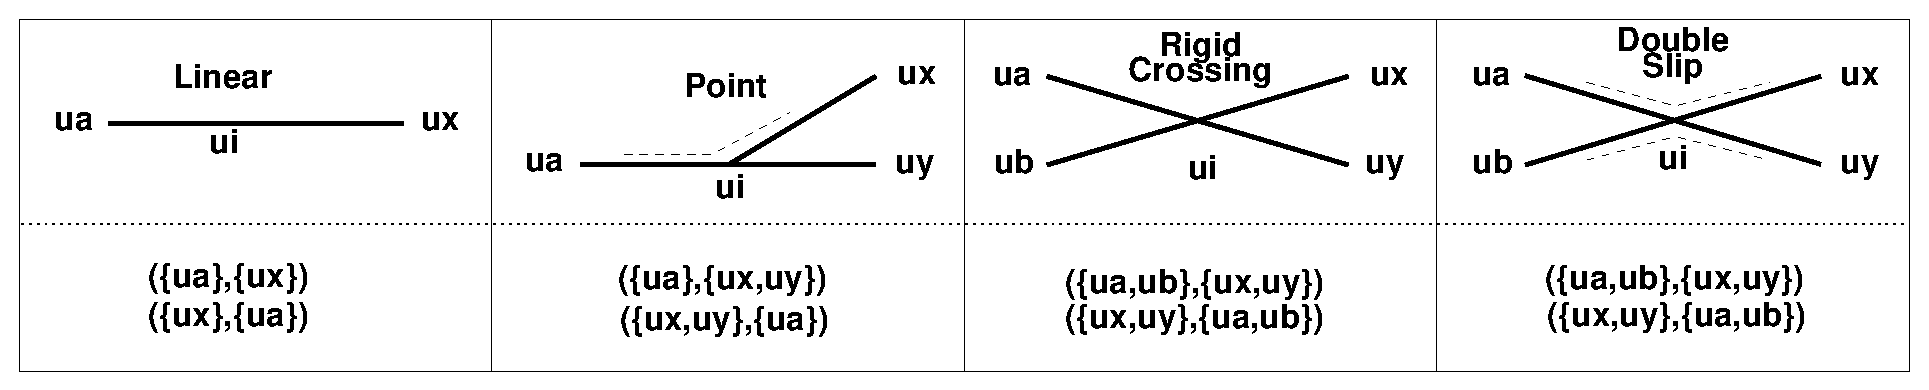
\epsfig{file=rail-mereo.eps,height=\pos{2.7}{5}cm}
\caption{Four Symmetric Rail Unit Mereologies\ \ \ \eod}\label{fig.rail-mereo}
\end{center}
\end{figure}

\label{lect3:labelmereo}

\pos{}{\mnewfoil
\label{lect3:label1a}
\ \vfill
\centerline{\lilacolor{Day \#{4}: Attributes and Summary}}
\vfill
}

\nbbbbb{Attributes}\label{chap4.Attributes}

\ysf{\dbeat{\pvienna{5.4}{119--139}}}

\noindent
\begynd
\pind To recall: there are three sets of
      \textbf{\pdindextermii{internal}{qualities}}:
\begynd
\pind \textsf{unique identifiers}, 
\pind \textsf{mereologies} and
\pind \textsf{attributes}. 
\afslut
\pind \textsf{Unique identifiers} and  \textsf{mereologies} \nyl
       are rather definite kinds of internal endurant qualities;
\pind \textsf{attributes} form more ``free-wheeling'' sets of
      \pdindextermii{internal}{qualities}.
\pind Whereas, for this \monograph, we suggest to not endow \nyl
fluids with unique identification and mereologies\ysfchg{. }

      \ysfchg{A}ll endurants, i.e., including fluids, are endowed with attributes. 
\afslut

\nbbbb{Inseparability of Attributes from Parts and Fluids}\label{technical issues}

\begynd
\pind Parts {and fluids} are 
\begynd
\pind typically recognised because of their spatial form
\pind and are otherwise characterised by their intangible, \nyl
      but measurable attributes. \pos{That is, whereas
      endurants, whether solid (as are parts) 
      or  fluids, are physical, tangible, in the sense of being
      spatial [or 
      being abstractions, i.e., concepts, of spatial endurants],
      attributes are intangible: cannot normally be
      touched\footnote{\LLLL One can see the red colour of a wall, but one
        touches the wall.}, or seen\footnote{One cannot see electric
        current, and one may touch an electric wire, but only if it
        conducts high voltage can one know that it is indeed an
        electric wire.}, but can
      be objectively measured\footnote{\LLLL That is, we restrict our domain
      analysis with respect to attributes to such quantities which are
      observable, say by mechanical, electrical or chemical
      instruments. Once objective measurements can be made of human
      feelings, beauty, and other, we may wish to include these
      ``attributes'' in our domain descriptions.}. Thus, in our quest
      for describing  
      domains where humans play an active r{\^o}le, we rule out
      subjective ``attributes'': feelings, sentiments, moods. Thus we
      shall abstain, in our domain science also from matters of
      aesthetics.}{} 
\afslut
    
 \pind We equate all endurants --- which have \nyl \LLLL \sfsl{the same type of unique
       identifiers, \nyl  the same type  of mereologies,  \nyl and the same types
       of attributes} \nyl \HHHH --- with one sort.
\pind Thus removing an internal quality from an endurant \nyl makes no sense:
\begynd \LLLL
\pind the endurant of that type 
\pind either becomes an endurant of another type
\pind or ceases to exist (i.e., becomes a non-entity)\,!
\afslut \HHHH
\mnewfoil

\pind We can roughly distinguish between two kinds of attributes:
\begynd
\pind those which can be motivated \nyl by \sort{physical}
      (incl\ysfchg{uding } chemical) \sort{concerns}, and
\pind those, \LLLL
\begynd
\pind which, although they embody some form of `physics measures',
\pind appear to reflect on \sort{event histories}: \LLLL
\begynd
\pind \sfsl{``if `something', $\phi$, has `happened' to an endurant, $e_a$,}
\pind \sfsl{then some `commensurate thing', $\psi$, has `happened' to
            another (one or more) endurants, $e_b$.''}
\afslut
\pind where the \sfsl{`something'} and \sfsl{`commensurate thing'}
\pind usually involve some `interaction' between the two (or more) endurants.
\afslut \HHHH
\pind It can take some reflection and analysis to properly identify \LLLL
\begynd
\pind endurants $e_a$ and $e_b$ and 
\pind commensurate events $\phi$ and $\psi$.
\afslut\HHHH
\pos{ 
\pind Example\,\ref{Intentional Pull -- Road Transport} shall illustrate the, as we shall call it,
      \bbcolor{intentional pull} of event histories.}{}
\afslut
\afslut

\nbbbb{Attribute Modelling Tools}\label{kap4.Attribute Modeling Tools}

\bbb{Attribute Quality and Attribute Value} \label{AQaAV} 
\begynd
\pind We distinguish between
\begynd
\pind an \bbcolor{attribute} (as a logical proposition, of a name, i.e.) \bbcolor{type}, and
\pind an \bbcolor{attribute value}, as a value in some value space.
\afslut
\afslut

\nbbb{Concrete Attribute Types}
\begynd
\pind By a \sfsl{concrete type}\pos{\index{dind}{concrete attribute
      type}\index{dind}{concrete!attribute!type}\index{dind}{type!concrete}\index{dind}{concrete!type}}{}
    \ysfchg{we } shall understand a sort (i.e., a type) which is defined in terms of
    some type expression: \textsf{T = $\mathcal{T}(...)$}.
\pind This is \ysf{indicated below by} \textsf{[=...]}.
\dbeat{We refer to
        Appendix Sect.\,\vref{tseb.rsl.Type Expressions} for more on \texttt{RSL} types.}
\afslut


\nbbb{Attribute Description}\label{pama:taf}\pos{\normalsize}{\HHHH}

\begynd
\pind Let us recall that attributes cover qualities \nyl other than
      unique identifiers and mereology.
\pind Let us then consider that parts and fluids \nyl \ysfchg{} have one or more attributes.
\begynd
\pind These attributes are qualities
\pind which help characterise ``what it means'' \nyl to be a part or a fluid.
\afslut 
\pind Note that we expect every part and fluid to have at least one attribute.
\pind The question is now, in general, \nyl how many and, particularly, which.
\afslut

\ysf{%%%
\begynd%%%
\pind The \bbcolor{\texttt{describe\_attributes}} description prompt
      is now defined.
\afslut%%%
}%%%

\mnewfoil\HHHH

\ddprompt{describe\_attributes}{observe-attributes}{\label{observeattributes}%%
\begynd\HHHH
\pind The domain analyser experiments, thinks and reflects \nyl about endurant,
      \textsf{e}, attributes. 
\pind That process is initiated by the \ddp:
\begin{itemize}
\item \texttt{describe\_attributes(e)}.\dodepr%
      \dpindex{describe\_attributes}%
\end{itemize}
\pind The result of that \ddp\ is \nyl that the domain analyser cum
      describer writes down \nyl the \ddtu{Attribute (Sorts or) Types and
        Observers}
\afslut
\mnewfoil\pos{}{\LLLL\HHHH}\bdbrule
\pos{}{{\bgcolor{\bgcolor{\cdlti}\ \texttt{describe\_attributes}} \sort{Observer}}}
      \delati{describe\_attributes}%
      \ddlt{PartAttributes}{dlti}
%\RSLatex
%let {&$\eta$A$_1$, ..., $\eta$A$_m$&} = determine_attribute_type_names(e) in     
%&\bq\kw{Narration:}&
%      [t]    ... &narrative text on attribute sorts& ...
%          &\,\,\,\,some \textsf{Ai}s may be concretely defined: [Ai=...]&
%      [o] &\,&  ... narrative text on attribute sort observers ...
%      [p] &\,&  ... narrative text on attribute sort proof obligations ...
%& \kw{Formalisation:}&
%      type
%      [t]   A&$_1$[=...]& , ...,  A&$_m$[=...]&
%      value
%      [o]   &{\attrmo}&A&$_1$&: E->A&$_1$&, ..., &{\attrmo}&A&$_m$&: E->A&$_m$&&\delaoi{\protect{\attrmo}}\label{attrAi}&
%      &\kw{proof obligation}& [Disjointness &of& Attribute Types]
%      [p]    &$\mathcal{PO}$:& &\poindex{podoats2}{\protect{$\mathcal{PO}:$} Disjointness of Attribute Types}&let P & be any part sort& in &[the domain description]&&\label{attribute-po}&
%      [p]            let a:(A&$_1$&|A&$_2$&|...|A&$_m$&) in &{\ismo}&A&$_i$&(a) ~= &{\ismo}&A&$_j$&(a) [i~=i, i,j:[1..m]] end end &\eq&
% end
%\endRSLatex 
\bp
\kw{let} {\LBRACE}$\eta$A$_1$, ..., $\eta$A$_m${\RBRACE} {\EQ} determine\_attribute\_type\_names(e) \kw{in}\ \ \ \ \ \\
\bq\kw{Narration:}\\
\>\>\>{\LBRACKET}t{\RBRACKET}\ \ \ \ {\DOTDOTDOT} narrative text on attribute sorts {\DOTDOTDOT}\\
\>\>\>\>\>\,\,\,\,some \textsf{Ai}s may be concretely defined: [Ai=...]\\
\>\>\>{\LBRACKET}o{\RBRACKET} \,\ \ {\DOTDOTDOT} narrative text on attribute sort observers {\DOTDOTDOT}\\
\>\>\>{\LBRACKET}p{\RBRACKET} \,\ \ {\DOTDOTDOT} narrative text on attribute sort proof obligations {\DOTDOTDOT}\\
 \kw{Formalisation:}\\
\>\>\>\kw{type}\\
\>\>\>{\LBRACKET}t{\RBRACKET}\ \ \ A$_1$[=...] , {\DOTDOTDOT},\ \ A$_m$[=...]\\
\>\>\>\kw{value}\\
\>\>\>{\LBRACKET}o{\RBRACKET}\ \ \ {\attrmo}A$_1$: E{\RIGHTARROW}A$_1$, {\DOTDOTDOT}, {\attrmo}A$_m$: E{\RIGHTARROW}A$_m$\delaoi{\protect{\attrmo}}\label{attrAi}\\
\>\>\>\kw{proof obligation} {\LBRACKET}Disjointness of Attribute Types{\RBRACKET}\\
\>\>\>{\LBRACKET}p{\RBRACKET}\ \ \ \ $\mathcal{PO}$: \poindex{podoats2}{\protect{$\mathcal{PO}:$} Disjointness of Attribute Types}\kw{let} P  be any part sort \kw{in} [the domain description]\label{attribute-po}\\
\>\>\>{\LBRACKET}p{\RBRACKET}\ \ \ \ \ \ \ \ \ \ \ \ \kw{let} a:(A$_1${\BAR}A$_2${\BAR}{\DOTDOTDOT}{\BAR}A$_m$) \kw{in} {\ismo}A$_i$(a) {\NOTEQ} {\ismo}A$_j$(a) {\LBRACKET}i{\NOTEQ}i, i,j:{\LBRACKET}1{\DOTDOT}m{\RBRACKET}{\RBRACKET} \kw{end} \kw{end} \eq\\
 \kw{end}
\ep
\edbrule
}

\noindent%
\pos{\psno}{\mnewfoil}%
\begynd%
\pind Let \textsf{A$_1$, ..., A$_n$} be the set of all
      conceivable attributes of endurant\ysfchg{ } $e$:$E$. 
\begynd
\pind (Usually $n$ is a
      rather large natural number, say in the order of a hundred
      conceivable such.) 
\pind In any one domain model the domain analyser
      cum describer selects a modest subset, \textsf{A$_1$,
        ..., A$_m$}, i.e., ${m}<{n}$. 
\pind Across many domain models \nyl for
      \textsl{``more-or-less the same''} domain $m$ varies \nyl and the
      attributes, \textsf{A$_1$,  ..., A$_m$}, \nyl selected for one
      model may differ \nyl from those, \textsf{A$'_1$, ..., A$'_{m'}$},
      chosen for another model.
\afslut
\mnewfoil
       
\pind The \kw{type} definitions: 
      \textsf{A$_1$, ..., A$_m$},
      inform us that the domain analyser has decided to focus
      on the distinctly named \textsf{A$_1$, ..., A$_m$}
      attributes.\pos{\footnote{\LLLL The attribute type names
      are chosen by the domain analyser to
      reflect on domain phenomena.}}{}
\pind The \kw{value} clauses 
\begynd
\pind \textsf{\small\HHHH{\attrmo}A$_1$:P{\RIGHTARROW}A$_1$, 
\pind  {\DOTDOTDOT},
\pind       {\attrmo}A$_n$:P{\RIGHTARROW}A$_n$} 
\afslut \normalsize\HHHH
      are then ``automatically'' given:
\begynd
\pind if an endurant, \textsf{e:E}, has an attribute \textsf{A$_i$}
\pind then there is postulated, ``by definition'' [eureka] 
      \pos{}{\\} an attribute
      observer function
      \textsf{\small\HHHH{\attrmo}A$_i$:E{\RIGHTARROW}A$_i$}
      et cetera\dbsquare\ 
\afslut
\afslut\pos{\normalsize}{\HHHH}
\mnewfoil

\begynd
\pind We cannot automatically, that is, syntactically, \nyl
      guarantee that our domain descriptions secure that
\begynd
\pind the various attribute types
\pind for a\ysfchg{n } endurant sort 
\pind denote disjoint sets of values. 
\afslut
      Therefore we must prove it. 
\afslut

\nbbb{Attribute Categories}\label{Attribute Categories}

\begynd
\pind Michael A.\ Jackson \cite{lexicon} has suggested a hierarchy of
      attribute categories:
\begynd
\pind from static
\pind to dynamic values -- and within the dynamic value category:
\begynd
\pind inert values,
\pind reactive values, 
\pind active values -- and within the dynamic active value category:
\begynd
\pind autonomous values,
\pind biddable values and
\pind programmable values.
\afslut
\afslut  
\afslut%
\pind We now review these attribute value types. \nyl
      The review is based on \pos{\cite[M.A.Jackson]{lexicon}}{\cite[M.A.Jackson]{lexicon}}.
\afslut%
\mnewfoil%

\begynd
\pind \sfsl{{Endurant attributes}} are 
\begynd
\pind either constant, i.e.,  \bmcolor{{static}}, 
\pind or varying, i.e., \bmcolor{{dynamic}}  
\afslut attributes\ysfchg{. }
\afslut
%%%
%%% STATIC
%%%

\attribute{static}{\begynd
\pind By a \label{staticattribute}
      {\pdindexii{static}{attribute}}, \textsf{{a:A}},
      \bbcolor{\protect{\texttt{is\_static\_attribute}}}({\textsf{a}}),%
      \sac\atindex{\protect{is\_static\_attribute}} \nyl
      we shall understand an attribute whose values
\begynd
\pind are constants,
\pind i.e., cannot change\dbsquare
\afslut
\afslut}
\mnewfoil
\monoexample{Static Attributes}{%
\begynd
\pind Let us exemplify road net attributes \nyl in this and the next examples.
\pind And let us assume the following attributes:
\begynd
\pind year of first link construction and
\pind link length at that time.
\afslut
\pind We may consider both to be static attributes:
\begynd
\pind The year first established, \nyl seems an obvious static attribute and
\pind the length is fixed at the time the road was first built.
\afslut
\afslut
}

%%%
%%% DYNAMIC
%%%
\mnewfoil\label{Dynamic Attribute Categories}
\attribute{dynamic}{\begynd\label{dynamicattribute}
  \pind By a {\pdindexii{dynamic}{attribute}}, \textsf{{a:A}},
      \bbcolor{\texttt{is\_dynamic\_attribute}}({\textsf{a}}),% 
      \sac\atindex{is\_dynamic\_attribute}\pos{}{\\}
      we shall understand an attribute whose values
\begynd
\pind are variable, 
\pind i.e., can change.
\afslut
{{Dynamic attributes}} are either \sfsl{inert, reactive}
or \sfsl{active} attributes\dbsquare
\afslut}
%%%%
%%%% INERT
%%%%
\mnewfoil
\attribute{inert}{
\begynd\label{inertattribute}
\pind By an \lilacolor{\pdindexii{inert}{attribute}}, \textsf{a:A},
      \bbcolor{\texttt{is\_\-in\-ert\_\-at\-tri\-bute}}(\textsf{a}),% 
      \sac\atindex{is\_inert\_attribute}\pos{}{\\}
      we shall understand a dynamic attribute whose values
\begynd
\pind only change as the result of external stimuli where 
\pind these stimuli prescribe new values\dbsquare
\afslut 
\afslut}
\mnewfoil
\monoexample{Inert Attribute}{%
\begynd
\pind And let us now further assume the following link attribute:
\begynd
\pind link name.
\afslut
\pind We may consider it to be an inert attribute:
\begynd
\pind the name is not ``assigned'' to the link by the link itself,
\pind but probably by some road net authority 
\pind which we are not modelling.
\afslut
\afslut
  }%%%
%%% REACTIVE
%%%
\mnewfoil
\attribute{reactive}{\label{reactiveattribute}
\begynd
\pind By a \bbcolor{\pdindexii{reactive}{attribute}}, \textsf{a:A}, 
      \bbcolor{\texttt{is\_reactive\_attribute}}(\textsf{a}),% 
      \sac\atindex{is\_reactive\_attribute}\pos{}{\\}
      we shall understand a dynamic attribute  whose values, 
\begynd
\pind if they vary, change  in response to external stimuli,
\pind where these stimuli  
\begynd
\pind either come from outside the domain of interest
\pind or from other endurants\dbsquare
\afslut
\afslut
\afslut
}
\mnewfoil

\monoexample{Reactive Attributes}{%
\begynd
\pind Let us further assume the following two link attributes:
\begynd
\pind ``wear and tear'', respectively
\pind ``icy and slippery''.
\afslut
\pind We will consider those attributes to be reactive in that
\begynd
\pind automobiles (another part) traveling the link, an external ``force'', \nyl
      typically causes the ``wear and tear'', respectively
\pind the weather (outside our domain) \nyl causes the  ``icy and slippery'' property.
\afslut
\afslut
}
%%%
%%% ACTIVE
%%%
\mnewfoil
\attribute{active}{\label{activeattribute}
\begynd
\pind By an \bbcolor{\pdindexii{active}{attribute}}, \textsf{a:A},
      \bbcolor{\texttt{is\_active\_attribute}}(\textsf{a}),% 
      \sac\atindex{is\_active\_attribute}\pos{}{\\}
      we shall understand a  dynamic attribute whose values 
\begynd
\pind change (also) \ysfchg{by } its own volition.
\afslut
{{Active attributes}} are 
\begynd
\pind either \sfsl{autonomous}, 
\pind or \sfsl{biddable} 
\pind or \sfsl{programmable}
\afslut attributes\dbsquare
\afslut}
%%%
%%% AUTONOMOUS
%%%
\mnewfoil
\attribute{autonomous}{\label{autonomousattribute}
\begynd
\pind By an \dindexii{autonomous}{attribute}, \textsf{a:A},
      \bbcolor{\texttt{is\_autonomous\_attribute}}(\textsf{a}),% 
      \sac\atindex{is\_autonomous\_attribute}\pos{}{\\}
      we shall understand a dynamic active attribute %\fromitemize 
\begynd
\pind whose values change only ``on their own volition''. 
\pind The values
      of an autonomous attributes \nyl are a ``law onto 
      themselves and their surroundings''\dbsquare
\afslut
\afslut}
\mnewfoil
\monoexample{Autonomous Attributes}{\LLLL\HHHH%
\begynd
\pind We enlarge \ysfchg{the } scope of our examples of attribute categories to now
      also include automobiles (on the road net).
\pind In this example we assume that an automobile is driven by a
      human [behaviour].
\pind These are some automobile attributes:
\begynd
\pind velocity,
\pind acceleration, and
\pind moving straight, or turning left, or turning right.
\afslut
\pind We shall consider these three attributes to be autonomous.
\begynd
\pind It is the driver, not the automobile, who decides
\pind whether the automobile should drive at constant velocity,
including 0, or accelerate or decelerate, including stopping.
\pind And it is the driver who decides when to turn left or right, or
not turn at all.
\afslut
\afslut
}
\mnewfoil
%%%
%%% BIDDABLE
%%%
\attribute{biddable}{\label{biddableattribute}
\begynd
\pind By a \lilacolor{\pdindexii{biddable}{attribute}}, \textsf{a:A},
      \bbcolor{\texttt{is\_\-bid\-dable\_\-at\-tri\-bute}}(\textsf{{\small\HHHH
          a}})\label{biddable}%  
      \sac\atindex{is\_biddable\_attribute} \nyl we shall understand a 
      {dynamic} {active} attribute whose values \faocb
\begynd
\pind \sfsl{are prescribed
\pind but may fail to be observed as \ysf{retaining that value}}\dbsquare
\afslut
\afslut}
\mnewfoil


\monoexample{Biddable Attributes}{In the context of automobiles these
  are some biddable attributes:
\begynd
\pind turning the wheel, to drive right at a hub \nyl -- with the
      automobile failing to turn right;
\pind pressing the accelerator, to obtain a higher speed \nyl --
      with the automobile failing to really gaining speed;
\pind pressing the brake, to stop \nyl --
      with the automobile failing to halt\dbsquare
\afslut}

%%%
%%% PROGRAMMABLE
%%%
\mnewfoil
\attribute{programmable}{\label{programmableattribute}
\begynd
\pind By a \lilacolor{\pdindexii{programmable}{attribute}},
      \textsf{a:A}, 
      \bbcolor{\texttt{is\_\-pro\-gram\-mable\_\-at\-tri\-bute}}(\textsf{a}),% 
      \sac\atindex{is\_programmable\_attribute}
      we shall understand a
      {dynamic} {active} attribute whose values
\begynd
\pind can be prescribed\dbsquare
\afslut
\afslut}
\mnewfoil
\monoexample{Programmable Attribute}{%
\begynd
\pind We continue with the automobile on the road net examples.
\pind In this example we assume that an automobile includes, as one
      inseparable entity, ``the driver''.
\pind These are some automobile attributes:
\begynd
\pind position on a link,
\pind velocity, acceleration (incl.\ deceleration), and
\pind direction: straight, turning left, turning right.
\afslut
\pind We shall now consider these three attributes to be programmable.
\afslut
}
\noindent
\pos{\psno}{\mnewfoil}
\begynd
\pind Figure\,\ref{attributes.fig} captures an attribute value ontology.
\afslut

\pos{\hDBfigure{attributes}{4cm}{Attribute Value Ontology}{attributes.fig}}%
    {\hDBfigure{attributes}{10cm}{Attribute Value Ontology}{attributes.fig}}


\noindent%
\pos{\psno}{\mnewfoil}%
\begynd%
\pind Figure\,\ref{attributes.fig} hints at three categories of
      dynamic attributes:
\begynd
\pind \bbcolor{monitorable only},
\pind \bbcolor{biddable} and
\pind \bbcolor{programmable}
\afslut
attributes.
\afslut
\mnewfoil

\attribute{monitorable only}{\label{monitorableattribute}
\begynd
\pind By a \lilacolor{\pdindexii{monitorable only}{attribute}},
      \textsf{a:A},  \nyl
      \bbcolor{\texttt{is\_monitorable\_only\_at\-tri\-bute}}(\textsf{a}),% 
      \sac\atindex{is\_monitorable\_only\_attribute} \nyl
      we shall understand a
      {dynamic} {active} attribute which is either
\begynd
\pind \sfsl{inert} or
\pind \sfsl{reactive} or
\pind \sfsl{autonomous}.
\afslut
\afslut} 
\noindent
That is:

%\RSLatex
%   value  
%      is_monitorable_only: E -> Bool
%      is_monitorable_only(e) is is_inert(e) \/ is_reactive(e) \/ is_autnomous(e)
%\endRSLatex 
\bp
\>\ \kw{value}\ \ \\
\>\>\>is\_monitorable\_only: E {\RIGHTARROW} \kw{Bool}\\
\>\>\>is\_monitorable\_only(e) {\IS} is\_inert(e) {\VEE} is\_reactive(e) {\VEE} is\_autonomous(e)
\ep


\mnewfoil

\monoexample{Road Net Attributes}
\noindent\LLLL\HHHH
\begynd
\pind We treat some attributes of the hubs of a road net.
\afslut
\begin{enumerate}\setei
\item \label{h-attr-000} There is a hub state.
\begynd
\pind  It is a set of pairs, \textsf{(l$_f$,l$_t$)}, of link identifiers,
\begynd
\pind  where these link identifiers are in the mereology of the hub. 
\afslut
\pind The meaning of the hub  state
\begynd
\pind in which, e.g., \textsf{(l$_f$,l$_t$)} is an element, 
\pind is that the hub is open,  \bgcolor{``green''}, 
\pind for traffic $f$rom link \textsf{l$_f$} $t$o link \textsf{l$_t$}.  
\pind If a hub state is empty
\pind then the hub is closed, i.e., \brcolor{``red''} 
\pind for traffic from any
                         connected links to any other connected links.
\afslut
\afslut
\pos{\psno}{\mnewfoil}
\item \label{h-attr-010} There is a hub state space.
\begynd
\pind It is a set of hub states. 
\pind The current hub state must be in its state space.
\pind The meaning of the hub state space is 
\begynd
\pind that its states are all those the hub can attain.
\afslut
\afslut
\item \label{hub-traffic} Since we can think rationally about it,
\begynd
\pind it can be described, hence we can model, as an
                          attribute of hubs, a history of its traffic:
\begynd
\pind the recording, per unique automobile identifier, 
\pind of the time ordered presence in the hub of these vehicles.   
\afslut
\pind Hub history is an \sfsl{event history}.
\afslut
\savei\end{enumerate}
\pos{\psno}{\mnewfoil}
\pos{\footsize}{\LLLL\HHHH\sf}
%\pos{\begin{multicols}{2}}{}
%\RSLatex
%type
%&\ref{h-attr-000}&  H`Sigma = (L_UI><L_UI)-set
%&\ref{h-attr-010}&  H`Omega = H`Sigma-set
%&\ref{hub-traffic}&  H_Traffic = A_UI -m-> (&$\mathbb{TIME}$& >< VPos)-list
%axiom
%&\ref{h-attr-000}&  all h:H :- obs_H`Sigma(h) isin obs_H`Omega(h)
%&\ref{hub-traffic}&  all ht:H_Traffic,ui:A_UI :-  ui isin dom ht => time_ordered(ht(ui))
%value 
%&\ref{h-attr-000}&  attr_H`Sigma: H -> H`Sigma
%&\ref{h-attr-010}&  attr_H`Omega: H -> H`Omega 
%&\ref{hub-traffic}&  attr_H_Traffic: H -> H_Traffic
%&\ref{hub-traffic}&   time_ordered: (&$\mathbb{TIME}$& >< VPos)-list -> Bool
%&\ref{hub-traffic}&   time_ordered(tvpl) is ...
%\endRSLatex  
\bp
\kw{type}\\
\ref{h-attr-000}\ \ H$\Sigma$ {\EQ} (L\_UI{\TIMES}L\_UI)\kw{-set}\\
\ref{h-attr-010}\ \ H$\Omega$ {\EQ} H$\Sigma$\kw{-set}\\
\ref{hub-traffic}\ \ H\_Traffic {\EQ} A\_UI {\MARROW} ($\mathbb{TIME}$ {\TIMES} VPos)$^{\ast}$\\
\kw{axiom}\\
\ref{h-attr-000}\ \ {\ALL} h:H {\RDOT} obs\_H$\Sigma$(h) {\ISIN} obs\_H$\Omega$(h)\\
\ref{hub-traffic}\ \ {\ALL} ht:H\_Traffic,ui:A\_UI {\RDOT}\ \ ui {\ISIN} \kw{dom} ht {\DBLRIGHTARROW} time\_ordered(ht(ui))\\
\kw{value} \\
\ref{h-attr-000}\ \ attr\_H$\Sigma$: H {\RIGHTARROW} H$\Sigma$\\
\ref{h-attr-010}\ \ attr\_H$\Omega$: H {\RIGHTARROW} H$\Omega$ \\
\ref{hub-traffic}\ \ attr\_H\_Traffic: H {\RIGHTARROW} H\_Traffic\\
\ref{hub-traffic}\ \ \ time\_ordered: ($\mathbb{TIME}$ {\TIMES} VPos)$^{\ast}$ {\RIGHTARROW} \kw{Bool}\\
\ref{hub-traffic}\ \ \ time\_ordered(tvpl) {\IS} {\DOTDOTDOT}
\ep
%\pos{\end{multicols}}{}
\pos{\normalsize}{\HHHH}\rm
\noindent
\begynd
\pind In Item\,\ref{hub-traffic} we model the time-ordered sequence
      of traffic as a discrete sampling, i.e., {\MARROW}, rather than as a
      continuous function, {\RIGHTARROW} \eod
\afslut

\pos{\psno}{\mnewfoil}
\monoexample{Invariance of Road Net Traffic States}{
\begynd
\pind We continue Example\,\vref{Road Net Attributes}.
\afslut
\begin{enumerate}\setei
\item \label{h-attr-030} The link identifiers of hub states must be in
                         the set, $l_{ui}s$, of the road net's link
                         identifiers.
\savei\end{enumerate}
%\RSLatex
%axiom
%&\ref{h-attr-030}&  all h:H :- h isin &$hs$& => 
%&\ref{h-attr-030}&      let h`sigma = attr_H`Sigma(h) in 
%&\ref{h-attr-030}&      all (l&$_{ui}i$&,li&$_{ui}i'$&):(L_UI><L_UI) :- (l&$_{ui}i$&,l&$_{ui}i'$&) isin h`sigma => {l&$_{ui_i}$&,l&$_{ui_i}'$&} <<= l&$_{ui}s$& end &\eod&
%\endRSLatex
\bp
\kw{axiom}\\
\ref{h-attr-030}\ \ {\ALL} h:H {\RDOT} h {\ISIN} $hs$ {\DBLRIGHTARROW} \\
\ref{h-attr-030}\ \ \ \ \ \ \kw{let} h$\sigma$ {\EQ} attr\_H$\Sigma$(h) \kw{in} \\
\ref{h-attr-030}\ \ \ \ \ \ {\ALL} (l$_{ui}i$,li$_{ui}i'$):(L\_UI{\TIMES}L\_UI) {\RDOT} (l$_{ui}i$,l$_{ui}i'$) {\ISIN} h$\sigma$ {\DBLRIGHTARROW} {\LBRACE}l$_{ui_i}$,l$_{ui_i}'${\RBRACE} {\SUBSETEQ} l$_{ui}s$ \kw{end} \eod
\ep
}%
\noindent%
\pos{\psno}{\mnewfoil}%
\begynd%
\pind You may skip Example\,\vref{Road Transport -- Further Attributes} in a first reading.
\afslut

\monoexample{Road Transport -- Further Attributes}{

  \bmcolor{Links:}

  We show just a few attributes.

\pos{\bmcii}{}
\begin{enumerate}\setei
\item \label{l-attr-000} There is a link state. It is a set of pairs,
                         \textsf{(h$_f$,h$_t$)}, of distinct hub identifiers,
                         where these hub identifiers are in the
                         mereology of the link. The meaning of a link
                         state in which \textsf{(h$_f$,h$_t$)} is an
                         element is that the link is open, 
                         \bgcolor{``green''}, for traffic $f$rom hub
                         \textsf{h$_f$} $t$o hub \textsf{h$_t$}.  Link
                         states can have either 0, 1 or 2 elements.
\item \label{l-attr-010} There is a link state space. It is a set of
                         link states.  The meaning of the link state
                         space is that its states are all those \ysf{}
                         which the link can attain. The current link state must be
                         in its state space. If a link state space is
                         empty then the link is \ysf{}
                         closed. If it has one element then it is a
                         one-way link. If a one-way link, $l$, is imminent
                         on a hub whose mereology designates that
                         link, then the link is a ``trap'', i.e., a
                         ``blind cul-de-sac''. 
\mnewfoil
\item \label{link-traffic} Since we can think rationally about it, it
                          can be described, hence it  can model, as an
                          attribute of links\ysf{,} a  history of its traffic:
                          the recording, per unique \ysf{}
                          automobile identifier, of the time ordered
                          positions along the link (from one hub to
                          the next) of these vehicles.  
\item \label{l-attr-030} The hub identifiers of link states must be in
                         the set, $h_{ui}s$, of the road net's hub
                         identifiers. 
\savei\end{enumerate}
\mnewfoil
\footsize\LLLL\HHHH
%\RSLatex
%type
%&\ref{l-attr-000}&  L`Sigma = (H_UI><H_UI)-set
%&\ref{l-attr-010}&  L`Omega = L`Sigma-set  
%&\ref{link-traffic}&  L_Traffic       
%&\ref{link-traffic}&  L_Traffic = A_UI -m-> (&$\mathbb{T}$&><(H_UI><Frac><H_UI))-list      
%&\ref{link-traffic}&  Frac = Real, axiom frac:Fract :- 0<frac<1
%value 
%&\ref{l-attr-000}&  attr_L`Sigma: L -> L`Sigma
%&\ref{l-attr-010}&  attr_L`Omega: L -> L`Omega
%&\ref{link-traffic}&  attr_L_Traffic: : -> L_Traffic
%axiom
%&\ref{l-attr-000}&  all l`sigma:L`Sigma:-card l`sigma<=2
%&\ref{l-attr-000}&  all l:L :- obs_L`Sigma(l) isin obs_L`Omega(l)
%&\ref{link-traffic}&  all lt:L_Traffic,ui:A_UI:-ui isin dom ht => time_ordered(ht(ui))
%&\ref{l-attr-030}&  all l:L:-l isin &$ls$& =>
%&\ref{l-attr-030}&     let l`sigma =attr_L`Sigma(l) in all (h&$_{ui}i$&,h&$_{ui}i'$&):(H_UI><H_UI):-&(h$_{ui}i$&,h&$_{ui}i'$)&isin l`sigma=>{h&$_{ui_i}$&,h&$_{ui_i}'$&}<<=h&$_{ui}s$& end
%\endRSLatex 
\bp
\kw{type}\\
\ref{l-attr-000}\ \ L$\Sigma$ {\EQ} (H\_UI{\TIMES}H\_UI)\kw{-set}\\
\ref{l-attr-010}\ \ L$\Omega$ {\EQ} L$\Sigma$\kw{-set}\ \ \\
\ref{link-traffic}\ \ L\_Traffic\ \ \ \ \ \ \ \\
\ref{link-traffic}\ \ L\_Traffic {\EQ} A\_UI {\MARROW} ($\mathbb{T}${\TIMES}(H\_UI{\TIMES}Frac{\TIMES}H\_UI))$^{\ast}$\ \ \ \ \ \ \\
\ref{link-traffic}\ \ Frac {\EQ} \kw{Real}, \kw{axiom} frac:Fract {\RDOT} 0{\LT}frac{\LT}1\\
\kw{value} \\
\ref{l-attr-000}\ \ attr\_L$\Sigma$: L {\RIGHTARROW} L$\Sigma$\\
\ref{l-attr-010}\ \ attr\_L$\Omega$: L {\RIGHTARROW} L$\Omega$\\
\ref{link-traffic}\ \ attr\_L\_Traffic: : {\RIGHTARROW} L\_Traffic\\
\kw{axiom}\\
\ref{l-attr-000}\ \ {\ALL} l$\sigma$:L$\Sigma${\RDOT}\kw{card} l$\sigma${\LEQ}2\\
\ref{l-attr-000}\ \ {\ALL} l:L {\RDOT} obs\_L$\Sigma$(l) {\ISIN} obs\_L$\Omega$(l)\\
\ref{link-traffic}\ \ {\ALL} lt:L\_Traffic,ui:A\_UI{\RDOT}ui {\ISIN} \kw{dom} ht {\DBLRIGHTARROW} time\_ordered(ht(ui))\\
\ref{l-attr-030}\ \ {\ALL} l:L{\RDOT}l {\ISIN} $ls$ {\DBLRIGHTARROW}\\
\ref{l-attr-030}\ \ \ \ \ \kw{let} l$\sigma$ {\EQ}attr\_L$\Sigma$(l) \kw{in} {\ALL} (h$_{ui}i$,h$_{ui}i'$):(H\_UI{\TIMES}H\_UI){\RDOT}(h$_{ui}i$,h$_{ui}i'$){\ISIN} l$\sigma${\DBLRIGHTARROW}{\LBRACE}h$_{ui_i}$,h$_{ui_i}'${\RBRACE}{\SUBSETEQ}h$_{ui}s$ \kw{end}
\ep
\pos{\emcii}{}\smallish\LLLL

\vspace*{1mm}
\mnewfoil

\noindent
\bmcolor{Automobiles:}
\begynd
\pind We illustrate but a few attributes:
\afslut
\begin{enumerate}\setei
\item \label{a-attr-000} Automobiles have static number plate
                         registration numbers.
\item \label{a-attr-005} Automobiles have dynamic positions on the road net:
\begin{enumerate}
\item\label{a-attr-005a} either \sfsl{at a hub} identified by some \textsf{h\_ui}, 
\item\label{a-attr-005b} or \sfsl{on a link}, some \sfsl{fraction, frac:Fract} down an
                         \sfsl{identified link, l\_ui}, from one of
                         its \sfsl{identified connecting hub}s, \textsf{fh\_ui}, in the 
                         direction of the other \sfsl{identified hub},
                         \textsf{th\_ui}. 
\item\label{a-attr-005c} Fraction is a real properly between 0 and 1.
\end{enumerate}
\savei\end{enumerate}\footsize
\mnewfoil

%\RSLatex
%type
%&\ref{a-attr-000}&   RegNo
%&\ref{a-attr-005}&   APos == atHub | onLink
%&\ref{a-attr-005a}&  atHub :: h_ui:H_UI &\pos{\tidxi{A: atHub::H\_UI}{a-attr-005a}}{}&
%&\ref{a-attr-005b}&  onLink :: fh_ui:H_UI >< l_ui:L_UI >< frac:Fract >< th_ui:H_UI&\pos{\tidxi{A: onLink::H\_UI{\TIMES}L\_UI{\TIMES}Fract{\TIMES}H\_UI}{a-attr-005b}}{}&
%&\ref{a-attr-005c}&  Fract = Real
%axiom
%&\ref{a-attr-005c}&  frac:Fract :- 0<frac<1 &\pos{\tidxi{A: Frac{\EQ}\kw{Real}}{a-attr-005 0}}{}&
%value  
%&\ref{a-attr-000}&   attr_RegNo: A -> RegNo&\pos{\afidxi{A: attr\_RegNo}{a-attr-000}}{}& 
%&\ref{a-attr-005}&   attr_APos: A -> APos&\pos{\afidxi{A: attr\_APos}{a-attr-005}}{}& 
%\endRSLatex 
\bp
\kw{type}\\
\ref{a-attr-000}\ \ \ RegNo\\
\ref{a-attr-005}\ \ \ APos {\EQ}{\EQ} atHub {\BAR} onLink\\
\ref{a-attr-005a}\ \ atHub :: h\_ui:H\_UI \pos{\tidxi{A: atHub::H\_UI}{a-attr-005a}}{}\\
\ref{a-attr-005b}\ \ onLink :: fh\_ui:H\_UI {\TIMES} l\_ui:L\_UI {\TIMES} frac:Fract {\TIMES} th\_ui:H\_UI\pos{\tidxi{A: onLink::H\_UI{\TIMES}L\_UI{\TIMES}Fract{\TIMES}H\_UI}{a-attr-005b}}{}\\
\ref{a-attr-005c}\ \ Fract {\EQ} \kw{Real}\\
\kw{axiom}\\
\ref{a-attr-005c}\ \ frac:Fract {\RDOT} 0{\LT}frac{\LT}1 \pos{\tidxi{A: Frac{\EQ}\kw{Real}}{a-attr-005 0}}{}\\
\kw{value}\ \ \\
\ref{a-attr-000}\ \ \ attr\_RegNo: A {\RIGHTARROW} RegNo\pos{\afidxi{A: attr\_RegNo}{a-attr-000}}{} \\
\ref{a-attr-005}\ \ \ attr\_APos: A {\RIGHTARROW} APos\pos{\afidxi{A: attr\_APos}{a-attr-005}}{} 
\ep
\mnewfoil\smallish\HHHH
\noindent
\begynd
\pind Obvious attributes that are not illustrated are those of
\begynd
\pind velocity and acceleration, 
\pind forward or backward movement, 
\pind turning right, left or going straight, 
\pind etc.
\afslut
\afslut
\mnewfoil
\noindent
\begynd
\pind The \sfsl{acceleration, deceleration, even velocity,} or \sfsl{turning 
      right, turning left, moving straight}, or \sfsl{forward} or
      \sfsl{backward} are seen as \sfsl{command actions}. 
\begynd
\pind As such they denote actions by the automobile ---
\pind such as \textsf{pressing the accelerator}, or \textsf{lifting
      accelerator pressure} or 
      \sfsl{braking}, or \sfsl{turning the wheel} in one direction or
      another, etc.
\pind As actions they have a kind of counterpart in the
      \textsf{vel}ocity, the \textsf{acc}eleration, etc. attributes.
\afslut
\afslut
\pos{\emcii}{}
\mnewfoil\smallish\HHHH
\begynd
\pind In Items\,\psref{hub-traffic} and \psref{link-traffic}, 
      we illustrated an aspect of domain 
      analysis \& description that may seem, and at least some decades
      ago would have seemed, strange: namely that if we can think,
      hence speak, about it, then we can model it ``as a fact'' in the
      domain. The case in point is that we include among hub and link
      attributes their histories of the timed whereabouts of \ysf{ }
      automobiles\footnotemark\dbsquare
\afslut
}\footnotetext{In this day and age of road cameras and
        satellite surveillance these traffic recordings may not appear
        so strange: We now know, at least in principle, of
        technologies that can record approximations to the hub and
        link traffic attributes.} 
\pos{\psno}{\mnewfoil}

\nbbb{Calculating Attribute Category Type Names}\label{Calculating Attribute Category Types}

                                %\input{attributes}

\begynd
\pind One can calculate sets of all attribute type names, of static,
      \ysf{} monitorable and programmable attribute types of parts and
      fluids with the following \dap{s}:
\begin{itemize}
\item \bcolor{\texttt{determine\_attr\_\ysfchg{names}}},
\item \bcolor{\texttt{sta\_attr\_types}},
\item \bcolor{\texttt{mon\_attr\_types}}, and
\item \bcolor{\texttt{pro\_attr\_types}}.
\end{itemize}
\noindent
\begynd
\pind \texttt{determine\_att\ysfchg{r}\_type\_names} applies to parts and
      yields a set of all attribute names of that part.
\pind \texttt{sta\_attr\_types} applies to parts and
      yields a set of attribute names of \sfsl{static} attributes
      of that part.\footnote{\LLLL $\eta\mathbb{A}$ is the type of all
      attribute types.}
\pind \texttt{mon\_attr\_types} applies to parts and
      yields a set of attribute names of \sfsl{monitorable} attributes
      of that part.
\pind \texttt{pro\_attr\_types} applies to parts and
      yields a set of attribute names of \sfsl{programmable} attributes
      of that part.
\afslut
\afslut
\mnewfoil
\dafprompt{determine\_attr\_type\_names}{analyse-attribute-types}{\label{analysisattributes}%%
%\RSLatex
%    value
%        determine_attr_type_names: P -> `eta&A&-set
%        determine_attr_type_names(p) as {`eta&A1&,`eta&A&,...,`eta&Am& }
%\endRSLatex
\bp
\>\>\kw{value}\\
\>\>\>\>determine\_attr\_type\_names: P {\RIGHTARROW} $\eta$A\kw{-set}\\
\>\>\>\>determine\_attr\_type\_names(p) \kw{as} {\LBRACE}$\eta$A1,$\eta$A,{\DOTDOTDOT},$\eta$Am {\RBRACE}
\ep
}

\mnewfoil
\dafprompt{sta\_attr\_type\_names}{sta-attr-types}{\label{staattrtypes}
%\RSLatex
%    value
%        sta_attr_type_names: P -> `eta&$\mathbb{A}$&><`eta&$\mathbb{A}$&><...><`eta&$\mathbb{A}$&
%        sta_attr_type_names(p) as (`eta&A1&,`eta&A2&,...,`eta&An&)&\label{static-attributes}&
%            &\kw{where:}&   {`eta&A1&,`eta&A2&,...,`eta&An&} <<= determine_attr_type_names(p)
%                  /\ let anms = determine_attribute_type_names(p)   
%                    all anm:`eta&$\mathbb{A}$& :- anm isin anms \ {`eta&A1&,`eta&A2&,...,`eta&An&}
%                      => ~ is_static_attribute{anm}
%                  /\ all anm:`eta&$\mathbb{A}$& :- anm isin {`eta&A1&,`eta&A2&,...,`eta&An&}
%                      => is_static_attribute{anm} end
%\endRSLatex 
\bp
\>\>\kw{value}\\
\>\>\>\>sta\_attr\_type\_names: P {\RIGHTARROW} $\eta$$\mathbb{A}${\TIMES}$\eta$$\mathbb{A}${\TIMES}{\DOTDOTDOT}{\TIMES}$\eta$$\mathbb{A}$\\
\>\>\>\>sta\_attr\_type\_names(p) \kw{as} ($\eta$A1,$\eta$A2,{\DOTDOTDOT},$\eta$An)\label{static-attributes}\\
\>\>\>\>\>\>\kw{where:}\ \ \ {\LBRACE}$\eta$A1,$\eta$A2,{\DOTDOTDOT},$\eta$An{\RBRACE} {\SUBSETEQ} determine\_attr\_type\_names(p)\\
\>\>\>\>\>\>\>\>\>{\WEDGE} \kw{let} anms {\EQ} determine\_attribute\_type\_names(p)\ \ \ \\
\>\>\>\>\>\>\>\>\>\>{\ALL} anm:$\eta$$\mathbb{A}$ {\RDOT} anm {\ISIN} anms {\SETMINUS} {\LBRACE}$\eta$A1,$\eta$A2,{\DOTDOTDOT},$\eta$An{\RBRACE}\\
\>\>\>\>\>\>\>\>\>\>\>{\DBLRIGHTARROW} {\SIM} is\_static\_attribute{\LBRACE}anm{\RBRACE}\\
\>\>\>\>\>\>\>\>\>{\WEDGE} {\ALL} anm:$\eta$$\mathbb{A}$ {\RDOT} anm {\ISIN} {\LBRACE}$\eta$A1,$\eta$A2,{\DOTDOTDOT},$\eta$An{\RBRACE}\\
\>\>\>\>\>\>\>\>\>\>\>{\DBLRIGHTARROW} is\_static\_attribute{\LBRACE}anm{\RBRACE} \kw{end}
\ep
}
\mnewfoil

\dafprompt{mon\_attr\_type\_names}{mon-attr-types}{\label{monattrtypes}
%\RSLatex  
%    value
%        mon_attr_type_names: P -> `eta&$\mathbb{A}$&><`eta&$\mathbb{A}$&><...><`eta&$\mathbb{A}$&
%        mon_attr_type_names(p) as (`eta&A1&,`eta&A2&,...,`eta&An&)&\label{monitorable-attributes}&
%            &\kw{where:}&   {`eta&A1&,`eta&A2&,...,`eta&An&} <<= determine_attr_type_names(p)
%                  /\ let anms = determine_attribute_type_names(p)   
%                    all anm:`eta&$\mathbb{A}$& :- anm isin anms \ {`eta&A1&,`eta&A2&,...,`eta&An&}
%                      => ~ is_monitorable_attribute{anm}
%                  /\ all anm:`eta&$\mathbb{A}$& :- anm isin {`eta&A1&,`eta&A2&,...,`eta&An&}
%                      => is_monitorable_attribute{anm} end
%\endRSLatex 
\bp
\>\>\kw{value}\\
\>\>\>\>mon\_attr\_type\_names: P {\RIGHTARROW} $\eta$$\mathbb{A}${\TIMES}$\eta$$\mathbb{A}${\TIMES}{\DOTDOTDOT}{\TIMES}$\eta$$\mathbb{A}$\\
\>\>\>\>mon\_attr\_type\_names(p) \kw{as} ($\eta$A1,$\eta$A2,{\DOTDOTDOT},$\eta$An)\label{monitorable-attributes}\\
\>\>\>\>\>\>\kw{where:}\ \ \ {\LBRACE}$\eta$A1,$\eta$A2,{\DOTDOTDOT},$\eta$An{\RBRACE} {\SUBSETEQ} determine\_attr\_type\_names(p)\\
\>\>\>\>\>\>\>\>\>{\WEDGE} \kw{let} anms {\EQ} determine\_attribute\_type\_names(p)\ \ \ \\
\>\>\>\>\>\>\>\>\>\>{\ALL} anm:$\eta$$\mathbb{A}$ {\RDOT} anm {\ISIN} anms {\SETMINUS} {\LBRACE}$\eta$A1,$\eta$A2,{\DOTDOTDOT},$\eta$An{\RBRACE}\\
\>\>\>\>\>\>\>\>\>\>\>{\DBLRIGHTARROW} {\SIM} is\_monitorable\_attribute{\LBRACE}anm{\RBRACE}\\
\>\>\>\>\>\>\>\>\>{\WEDGE} {\ALL} anm:$\eta$$\mathbb{A}$ {\RDOT} anm {\ISIN} {\LBRACE}$\eta$A1,$\eta$A2,{\DOTDOTDOT},$\eta$An{\RBRACE}\\
\>\>\>\>\>\>\>\>\>\>\>{\DBLRIGHTARROW} is\_monitorable\_attribute{\LBRACE}anm{\RBRACE} \kw{end}
\ep
}

\mnewfoil
\dafprompt{pro\_attr\_type\_names}{pro-attr-types}{\label{proattrtypes}
%\RSLatex
%    value
%        pro_attr_type_names: P -> `eta&$\mathbb{A}$&><`eta&$\mathbb{A}$&><...><`eta&$\mathbb{A}$&
%        pro_attr_type_names(p) as (`eta&A1&,`eta&A2&,...,`eta&An&)&\label{programmable-attributes}&
%            &\kw{where:}&   {`eta&A1&,`eta&A2&,...,`eta&An&} <<= determine_attr_type_names(p)
%                  /\ let anms = determine_attribute_type_names(p)   
%                    all anm:`eta&$\mathbb{A}$& :- anm isin anms \ {`eta&A1&,`eta&A2&,...,`eta&An&}
%                      => ~ is_monitorable_attribute{anm}
%                  /\ all anm:`eta&$\mathbb{A}$& :- anm isin {`eta&A1&,`eta&A2&,...,`eta&An&}
%                      => is_monitorable_attribute{anm} end
%\endRSLatex 
\bp
\>\>\kw{value}\\
\>\>\>\>pro\_attr\_type\_names: P {\RIGHTARROW} $\eta$$\mathbb{A}${\TIMES}$\eta$$\mathbb{A}${\TIMES}{\DOTDOTDOT}{\TIMES}$\eta$$\mathbb{A}$\\
\>\>\>\>pro\_attr\_type\_names(p) \kw{as} ($\eta$A1,$\eta$A2,{\DOTDOTDOT},$\eta$An)\label{programmable-attributes}\\
\>\>\>\>\>\>\kw{where:}\ \ \ {\LBRACE}$\eta$A1,$\eta$A2,{\DOTDOTDOT},$\eta$An{\RBRACE} {\SUBSETEQ} determine\_attr\_type\_names(p)\\
\>\>\>\>\>\>\>\>\>{\WEDGE} \kw{let} anms {\EQ} determine\_attribute\_type\_names(p)\ \ \ \\
\>\>\>\>\>\>\>\>\>\>{\ALL} anm:$\eta$$\mathbb{A}$ {\RDOT} anm {\ISIN} anms {\SETMINUS} {\LBRACE}$\eta$A1,$\eta$A2,{\DOTDOTDOT},$\eta$An{\RBRACE}\\
\>\>\>\>\>\>\>\>\>\>\>{\DBLRIGHTARROW} {\SIM} is\_monitorable\_attribute{\LBRACE}anm{\RBRACE}\\
\>\>\>\>\>\>\>\>\>{\WEDGE} {\ALL} anm:$\eta$$\mathbb{A}$ {\RDOT} anm {\ISIN} {\LBRACE}$\eta$A1,$\eta$A2,{\DOTDOTDOT},$\eta$An{\RBRACE}\\
\>\>\>\>\>\>\>\>\>\>\>{\DBLRIGHTARROW} is\_monitorable\_attribute{\LBRACE}anm{\RBRACE} \kw{end}
\ep
}


      

\mnewfoil
\noindent
\begynd
\pind Some comments are in order.
\begynd
\pind The \textsf{analyse\_attribute\_type\_names} function is, as
      throughout, meta-linguistic, that is, informal, not-computable,
      but decidable by the domain \ysf{modeller}. Applying it
      to a part or fluid yields, at the discretion of the domain
      \ysf{modeller}, a set of attribute type names ``freely''
      chosen by the domain \ysf{modeller}.
\pind The \textsf{sta\_attr\_type\_names}, the
          \textsf{mon\_attr\_type\_names}, and the
          \textsf{pro\_attr\_type\_names} functions are likewise
      meta-linguistic; their definition here relies on the
      likewise meta-linguistic \textsf{is\_static,
      is\_monitorable} and \textsf{is\_programmable} analysis predicates.
\afslut
\afslut

\nbbb{Calculating Attribute Values}\label{Calculating Attribute Values}

%\input{attributes-2}

\begynd
\pind Let
      \textsf{($\eta$A1, $\eta$A2, {\DOTDOTDOT} , $\eta$An)} be
      a grouping of attribute types for part $p$ (or fluid $f$).
\pind Then \textsf{{(attr\_A1(p), attr\_A2(p), {\DOTDOTDOT} ,attr\_An(p))}}
\pind (respectively \textsf{f})
\pind yields \textsf{(a1, a2, {\DOTDOTDOT} , an)}, the grouping
      of values for these attribute types.

\pind We can ``formalise'' this conversion:

%\RSLatex
%   value
%      types_to_values: `eta&$\mathbb{A}_1$& >< `eta&$\mathbb{A}_2$& >< ... >< `eta&$\mathbb{A}_n$& -> A&$_1$& >< A&$_2$& >< ... >< A&$_n$&
%\endRSLatex 
\bp
\>\ \kw{value}\\
\>\>\>types\_to\_values: $\eta$$\mathbb{A}_1$ {\TIMES} $\eta$$\mathbb{A}_2$ {\TIMES} {\DOTDOTDOT} {\TIMES} $\eta$$\mathbb{A}_n$ {\RIGHTARROW} A$_1$ {\TIMES} A$_2$ {\TIMES} {\DOTDOTDOT} {\TIMES} A$_n$
\ep

\afslut

\nbbbb{Operations on Monitorable Attributes of Parts}\label{OoPDAs}

\begynd
\pind We remind the \pos{reader}{student} of the notions  of 
\begynd 
\pind states in general, Sect.\,\ref{kap3.States.general} and \ysf{of}
\pind updateable states, Sect.\,\vref{kap3.States.specific}\ysf{ in specific}.
\begynd
\pind For every domain description there \ysf{is} possibly \ysf{} an updateable state.
\pind The\ysf{re} is such a state if there is at least one part with at least
      one monitorable attribute.
\afslut
\pind Below\pos{, as in Sect.\,\ref{kap3.States.specific},}{} we refer to the
      updateable states as $\sigma$.
\afslut
\afslut

\mnewfoil

\begynd
\pind Given a part, \textsf{p}, with attribute \textsf{A},
\begynd
\pind the simple operation \textsf{attr\_A(p)} 
\pind thus yields the value of attribute \textsf{A}
\pind for that part.
\afslut
\pind But what if, \ysf{if} what we have is just 
\begynd
\pind the global state $\sigma$\ysf{} of the set of all monitorable parts of a given
      universe-of-discourse, \textsf{uod},
\pind the unique identifier, \textsf{uid\_P(p)}, of a part of $\sigma$, and
\pind the name, \textsf{$\eta$A}, of an attribute of \textsf{p}\,?
\begynd
\pind Then how do we
\begynd
\pind ascertain the attribute value for \textsf{A} of \textsf{p},
\pind and, for \sfsl{biddable} attributes \textsf{A},
\pind ``update'' \textsf{p}, in $\sigma$, to some \textsf{A} value\,?
\afslut
\pind Here is how we express these two issues.
\afslut
\afslut
\afslut

\bbb{Evaluation of Monitorable Attributes}\label{Evaluation of Monitorable Attributes}

\begin{enumerate}\setei
\item \label{us000} Let \textsf{pi:PI} be the unique identifier of any
  part, $p$, with monitorable attributes, let \textsf{A} be a
  monitorable attribute of $p$, and let \textsf{$\eta$A} be the name
  of attribute \textsf{A}.
\item \label{us010} Evaluation of the [current] attribute  \textsf{A}
  value of $p$ is defined by function \textsf{read\_A\_from\_P} --
  \textsf{retr\_part(pi)} is defined in Sect.\,\vref{Part Retrieval}.
\savei\end{enumerate}

%\RSLatex
%value
%&\ref{us000}.&    pi:PI, a:A, `eta&A&:`eta&$\mathbb{T}$&
%
%&\ref{us010}.&    read_A_from_P: PI >< &$\mathbb{T}$& -> read `sigma A &\label{readA}&
%&\ref{us010}.&    read_A(pi,`eta&A&) is attr_A(retr_part(pi))
%\endRSLatex
\bp
\kw{value}\\
\ref{us000}.\ \ \ \ pi:PI, a:A, $\eta$A:$\eta$$\mathbb{T}$\\
\\
\ref{us010}.\ \ \ \ read\_A\_from\_P: PI {\TIMES} $\mathbb{T}$ {\RIGHTARROW} \kw{read} $\sigma$ \label{readA}\\
\ref{us010}.\ \ \ \ read\_A(pi,$\eta$A) {\IS} attr\_A(retr\_part(pi))
\ep
        
\nbbb{Update of Biddable Attributes}\label{Update of Biddable Attributes}

\begin{enumerate}\setei
\item \label{us040} The update of a monitorable attribute \textsf{A},
  with attribute name \textsf{$\eta$A}
  of part $p$, identified by \textsf{pi}, to a new value \kw{write}s
  to the global part state $\sigma$. 
\item \label{us060} Part $p$ is retrieved from the global state.
\item \label{us070} A new part, \textsf{p$'$} is formed such that
  \textsf{p$'$} is like part \textsf{p}:
\begin{enumerate}
\item \label{us080} same unique identifier, 
\item \label{us081} same mereology,
\item \label{us082} same attributes values,
\item \label{us083} except for \textsf{A}.
\end{enumerate}
\item \label{us100} That new $p'$ replaces $p$ in $\sigma$.
\savei\end{enumerate}

\mnewfoil\LLLL\HHHH

%\RSLatex
%value
%&\ref{us000}.&    `sigma, a:A, pi:PI, `eta&A&:`eta&$\mathbb{T}$&
%
%&\ref{us040}.&    update_P_with_A: PI >< A >< &$\eta\mathbb{T}$& -> write `sigma &\label{updatePwithA}&  
%&\ref{us040}.&    update_P_with_A(pi,a,`eta&A&) is
%&\ref{us060}.&        let p = retr_part(pi) in
%&\ref{us070}.&        let p&$'$&:P :-  
%&\ref{us080}.&            uid_P(p&$'$&)=pi 
%&\ref{us081}.&            /\ mereo_P(p)=mereo_P(p&$'$&)
%&\ref{us082}.&            /\ all `eta&A$'$& isin analyse_attribute_type_names(p) \ {`eta&A&} => attr_A&$'$&(p)=attr_A&$'$&(p&$'$&)
%&\ref{us083}.&            /\ attr_A(p')=a in
%&\ref{us100}.&        `sigma := `sigma \ {p} union {p'}
%&\ref{us040}.&        end end
%\endRSLatex 
\bp
\kw{value}\\
\ref{us000}.\ \ \ \ $\sigma$, a:A, pi:PI, $\eta$A:$\eta$$\mathbb{T}$\\
\\
\ref{us040}.\ \ \ \ update\_P\_with\_A: PI {\TIMES} A {\TIMES} $\eta\mathbb{T}$ {\RIGHTARROW} \kw{write} $\sigma$ \label{updatePwithA}\ \ \\
\ref{us040}.\ \ \ \ update\_P\_with\_A(pi,a,$\eta$A) {\IS}\\
\ref{us060}.\ \ \ \ \ \ \ \ \kw{let} p {\EQ} retr\_part(pi) \kw{in}\\
\ref{us070}.\ \ \ \ \ \ \ \ \kw{let} p$'$:P {\RDOT}\ \ \\
\ref{us080}.\ \ \ \ \ \ \ \ \ \ \ \ uid\_P(p$'$){\EQ}pi \\
\ref{us081}.\ \ \ \ \ \ \ \ \ \ \ \ {\WEDGE} mereo\_P(p){\EQ}mereo\_P(p$'$)\\
\ref{us082}.\ \ \ \ \ \ \ \ \ \ \ \ {\WEDGE} {\ALL} $\eta$A$'$ {\ISIN} analyse\_attribute\_type\_names(p) {\SETMINUS} {\LBRACE}$\eta$A{\RBRACE} {\DBLRIGHTARROW} attr\_A$'$(p){\EQ}attr\_A$'$(p$'$)\\
\ref{us083}.\ \ \ \ \ \ \ \ \ \ \ \ {\WEDGE} attr\_A(p{\PRIM}){\EQ}a \kw{in}\\
\ref{us100}.\ \ \ \ \ \ \ \ $\sigma$ :{\EQ} $\sigma$ {\SETMINUS} {\LBRACE}p{\RBRACE} {\UNION} {\LBRACE}p{\PRIM}{\RBRACE}\\
\ref{us040}.\ \ \ \ \ \ \ \ \kw{end} \kw{end}
\ep
%%%%%%%%%%%%%%%%%%%%%%%%%%%%%%%%%%%%%%%%%

     
\nbbb{Stationary and Mobile Attributes}\label{Stationary and Mobile Attributes}%% Added 17 Sept. 2022 !!!



\begynd
\pind  Endurants are either \bbcolor{stationary} or
       \bbcolor{mobile}.\pos{\footnote{This section was added on
       Sept.\,17, 2022\,!}}{} 
\afslut

\bookdefn{Stationary}{ An endurant is said to be stationary if it never moves\dbsquare}

\noindent
\begynd
\pind Being stationary is a static attribute.
\afslut

\daprompt{is\_stationary}{is-stationary}{\label{is stationary}%
\begynd
\pind The method provides the \dap:
\begin{itemize}
\item \bcolor{\texttt{is\_stationary}}
     \doanpr\pos{\apindex{is\_stationary}}{}
      -- where 
      \texttt{is\_stationary($e$)} \nyl  holds if $e$ is to be considered stationary\eoap
\end{itemize}
\afslut
}

\mnewfoil

\monoexample{Stationary Endurants}{%
\begynd
\pind Examples of stationary endurants could be:
\begynd
\pind \pos{(i)}{} road hubs and links;
\pind \pos{(ii)}{} container terminal stacks;
\pind \pos{(iii)}{} pipeline units; and
\pind \pos{(iv)}{} sea, lake and river beds\dbsquare
\afslut
\afslut}

\mnewfoil

\bookdefn{Mobile}{ An endurant is said to be mobile if it is capable of
  being moved -- whether by its own \ysf{volition}, or otherwise\dbsquare}
\noindent
\begynd
\pind Being mobile is a static attribute.
\afslut

\daprompt{is\_mobile}{is-mobile}{\label{is mobile}%
\begynd
\pind The method provides the \dap:
\begin{itemize}
\item \bcolor{\texttt{is\_mobile}}
     \doanpr\pos{\apindex{is\_mobile}}{} -- where 
      \texttt{is\_mobile($e$)} \nyl  holds if $e$ is to be considered mobile\eoap
\end{itemize}
\afslut
}

\mnewfoil

\monoexample{Mobile Endurants}{%
\begynd
\pind Examples of mobile endurants are:
\begynd
\pind \pos{(i)}{} automobiles;
\pind \pos{(ii)}{} container terminal vessels, containers, cranes and trucks;
\pind \pos{(iii)}{} pipeline oil (or gas, or water, ...);
\pind \pos{(iv)}{} sea, lake and river water\dbsquare
\afslut
\afslut}

\noindent
\begynd
\pind Being stationary or mobile is an attribute of any manifest endurant.
\begynd
\pind Fo\ysf{r} every manifest endurant, $e$, it is the case that
\pind \texttt{is\_stationary(e){\IS}{\SIM}is\_mobile(e)}.
\afslut
\afslut

\treprikker

\mnewfoil

\noindent
\begynd
\pind Being stationary or, vice-versa, being mobile \nyl is often \bbcolor{tacitly assumed.}
\begynd
\pind Having external or internal qualities of a certain kind \nyl is often
      also tacitly assumed.
\pind A major point of the domain analysis \& description approach,
\begynd
\pind of \pos{this primer}{these lectures},
\pind is to help the domain \ysf{modeller} --
\pind the domain engineer cum researcher --
\pind to unveil as many, if not all, these qualities.
\afslut
\pind \bbcolor{Tacit understanding} would not be a common problem \nyl
      was it not for us to practice it ``excessively''\,!
\afslut
\afslut

%\nbbbb{Physics Attributes}

\nbbbb{Physics Attributes}\label{si}\label{si.1}\pos{\normalsize}{}

\begynd
\pind In this section we shall muse 
\begynd
\pind about the kind of attributes that
      are typical of natural parts,
\pind but which may also be relevant as attributes of artefacts.
\afslut

\pind Typically, when physicists write computer programs,
\begynd
\pind intended for calculating physics behaviours,
\pind they ``lump'' all of these into the \sort{type} \sort{Real},
\pind thereby hiding some important physics 'dimensions'.
\pind In this section we shall review that which is missing\,!
\afslut
\afslut

\pos{\psno}{\mnewfoil}
\begynd
\pind The subject of physical dimensions in programming languages \nyl
      is rather decisively treated in David Kennedy's 1996 PhD Thesis
      \cite{Kennedy96} ---
\pind so there really is no point in trying to cast new light on this subject
\pind other than to remind the reader of what these physical
      dimensions are all about.
\afslut

\nbbb{SI: The International System of Quantities}\label{si-1}

\begynd
\pind In physics we operate on \nyl values of attributes of manifest,
      i.e., physical phenomena. \pos{
\pind The type of some of these attributes are recorded \nyl in well
      known tables, cf.\,Tables\,\ref{table:1}--\ref{table:3}.}{}
\afslut
%\mnewfoil
\pos{Table\,\vref{table:1} shows the base units of physics.}{}

\pos{\footnotesize}{\HHHH}
\begin{table}[h]\HHHH
  \centering
\begin{tabular}{|lll|} \hline
Base quantity     &          Name   &      Type \\ \hline
length            &          meter   &     m \\
mass              &          kilogram   &  kg \\
time              &          second  &     s \\
electric current     &       ampere   &    A \\
thermodynamic temperature &  kelvin  &     K \\
amount of substance    &     mole    &     mol \\
luminous intensity     &     candela &     cd \\ \hline
\end{tabular} \caption{\HHHH Base SI Units} \label{table:1}
\end{table}
\normalsize\HHHH
\mnewfoil
\noindent
\pos{Table\,\vref{table:2} shows the units of physics derived from the base units.}{}
\pos{\footnotesize}{\HHHH\LLLL}%%%
\begin{table}[h]\LLLL\LLll
  \centering
\begin{tabular}{|llll|} \hline
         Name   &      Type & Derived Quantity & Derived Type \\ \hline
         radian & rad & angle & m/m  \\ 
         steradian & sr & solid angle & m$^2\times$m$^{-2}$ \\  
         Hertz  & Hz  & frequency & s$^{-1}$ \\
         newton & N   & force, weight   & kg{$\times$}m{$\times$}s$^{-2}$ \\
         pascal & Pa & pressure, stress & N/m$^2$ \\
         joule  & J & energy, work, heat & N$\times$m \\
         watt   & W & power, radiant flux &     J/s \\
         coulomb & C & electric charge & s$\times$A \\
volt &  V & electromotive force &  W/A (kg$\times$m$^2\times$s$^{-3}\times$A$^{-1}$) \\
farad & F & capacitance & C/V (kg$^{-1}\times$·m$^{-2}\times$s$^4\times$A$^2$) \\
ohm & $\Omega$ &  electrical resistance & V/A (kg$\times$m$^2\times$s$^{−3}\times$A$^{−2}$) \\
siemens & S & electrical conductance & A/V (kg${−1}\times$m$^{−2}\times$s$^3\times$A$^2$)\\
weber & Wb & magnetic flux &  V$\times$s  (kg$\times$m$^2\times$s$^{-2}\times$A$^{-1}$)\\
tesla   & T &  magnetic flux density   & Wb/m$^2$ (kg$\times$s$^{−2}\times$A$^{-1}$) \\
henry   & H &  inductance    &   Wb/A (kg$\times$m$^2\times$s$^{-2}\times$A$^2$) \\
degree Celsius    &     $^o$C    &   temp.\ rel.\ to 273.15 K & K \\
lumen &  lm  &   luminous flux   & cd$\times$sr   (cd) \\
lux   &  lx  & illuminance   &   lm/m$^2$   (m$^{−2}\times$cd) \\ \hline
\end{tabular}  \caption{\HHHH Derived SI Units} \label{table:2}
\end{table}
\mnewfoil 
\noindent\pos{\normalsize}{\HHHH\LLLL}
\pos{Table\,\ref{table:3} shows further units of physics derived from the base units.}{}
 \pos{\footnotesize}{\large\HHHH}
\begin{table}[h]\HHHH\LLLL
  \centering
\begin{tabular}{|lll|} \hline
Name   &  Explanation & Derived Type \\ \hline
area                               & square meter                &    m$^2$ \\
volume                             & cubic meter                 &    m$^3$ \\
speed                              & meter per second            &    m/s \\
wave number                        & reciprocal meter            &    m-1 \\
mass density                       & kilogram per cubic meter    &    kg/m$^3$ \\
specific volume                    & cubic meter per kilogram    &    m3/kg \\
current density                    & ampere per square meter     &    A/m$^2$ \\
magnetic field strength            & ampere per meter            &    A/m \\
substance concentration            & mole per cubic meter        &    mol/m$3$ \\
luminance                          & candela per square meter    &    cd/m$^2$ \\
mass fraction                      & kilogram per kilogram       &    kg/kg = 1 \\ \hline
\end{tabular}
  \caption{\HHHH Further SI Units}
  \label{table:3}
\end{table}
\mnewfoil
\noindent
\pos{\sfsl{velocity} is speed with three dimensional direction and is,
  for example, given as
\begin{itemize}
\item \sfsl{velocity}, \sf meter per second \rm with \sf direction\rm: \hfill $m/s$
\item \sfsl{acceleration},  \sf meter per second squared\rm, \hfill  $ m/s^2$
\item \sfsl{(longitude,latitude,azimuth)} measured in \sf radian\rm: \hfill  $(r,r,r)$ 
\end{itemize}}{}

\noindent
\pos{\normalsize Table\,\ref{table:4} shows standard
prefixes for SI units of measure 
and Tables\,\ref{table:6} show
fractions of SI units.}{}

\pos{\scriptsize}{\large\HHHH\LLLL}
%\pos{\begin{multicols}{2}}{}

\begin{table}[h]\HHHH\center
\begin{tabular}{|lllllll|} \hline
Prefix name   &      & deca  &  hecto &  kilo &   mega &   giga \\
Prefix symbol &      & da    &  h  &     k   &    M   &    G  \\
Factor        & 10$^0$ & 10$^1$ & 10$^2$ & 10$^3$ & 10$^6$  & 10$^9$\\ \hline
Prefix name   &      &   tera  &  peta  &  exa  &   zetta &  yotta\\
Prefix symbol &      &    T  &     P &      E &      Z &     Y\\
Factor        &&  10$^{12}$  & 10$^{15}$ & 10$^{18}$ & 10$^{21}$ & 10$^{24}$\\ \hline
\end{tabular} \ \ \
  \caption{\HHHH Standard Prefixes for SI Units of Measure}
  \label{table:4}
\end{table}

\dbeat{
\pos{\psno}{\mnewfoil}
\begin{table}[h]\LLLL\HHHH\center
\begin{tabular}{|lllllll|} \hline
Prefix name      &    &   deci  &  centi  & milli &  micro &  nano   \\
Prefix symbol     &   &   d   &    c  &     m   &    $\mu$ &       n   \\
Factor        & 10$^0$ & 10$^{-1}$ & 10$^{-2}$ & 10$^{-3}$ & 10$^{-6}$ & 
10$^{-9}$   \\ \hline
Prefix name      &    &     pico &   femto &  atto &   zepto  & yocto\\
Prefix symbol     &   &          p &      f &      a &      z    &   y\\
Factor        &  &  10$^{-12}$  & 10$^{-15}$ & 10$^{-18}$ & 10$^{-21}$ &
10$^{-24}$\\ \hline
\end{tabular}
  \caption{\HHHH Fractions}
  \label{table:5}
\end{table}
%\pos{\end{multicols}}{}
}


\normalsize
\mnewfoil
%\fest{%\begin{multicols}{2}
\begin{table}[h]\LLll\center
\begin{tabular}{|lllllll|} \hline %\hline
Prefix name   &      & deca  &  hecto &  kilo &   mega &   giga \\
Prefix symbol &      & da    &  h  &     k   &    M   &    G  \\
Factor        & 10$^0$ & 10$^1$ & 10$^2$ & 10$^3$ & 10$^6$  & 10$^9$\\ \hline
Prefix name   &      &   tera  &  peta  &  exa  &   zetta &  yotta\\
Prefix symbol &      &    T  &     P &      E &      Z &     Y\\
Factor        &&  10$^{12}$  & 10$^{15}$ & 10$^{18}$ & 10$^{21}$ & 10$^{24}$\\ \hline\hline
Prefix name      &    &   deci  &  centi  & milli &  micro &  nano   \\
Prefix symbol     &   &   d   &    c  &     m   &    $\mu$ &       n   \\
Factor        & 10$^0$ & 10$^{-1}$ & 10$^{-2}$ & 10$^{-3}$ & 10$^{-6}$ & 
10$^{-9}$   \\ \hline
Prefix name      &    &     pico &   femto &  atto &   zepto  & yocto\\
Prefix symbol     &   &          p &      f &      a &      z    &   y\\
Factor        &  &  10$^{-12}$  & 10$^{-15}$ & 10$^{-18}$ & 10$^{-21}$ &
10$^{-24}$\\ \hline
\end{tabular}
  \caption{\HHHH SI Units of Measure and Fractions}
  \label{table:6}
\end{table}
\normalsize\HHHH
\mnewfoil
\treprikker
\noindent
\begynd
\pind The point in \ysfchg{including } this material is
\begynd
\pind that when modelling, i.e., describing domains
\pind we must be extremely careful in not falling into the trap
\pind of modelling physics types, etc.,  as we do in programming --
\pind by simple \sort{Real}s.
\afslut
\pind We claim, without evidence, 
\begynd
\pind that many trivial programming mistakes
\pind are due to confusions between especially 
\pind derived SI units, fractions and prefixes.
\afslut
\afslut

\nbbb{Units are Indivisible}
\begynd
\pind A volt, kg$\times$m$^2\times$s$^{-3}\times$A$^{-1}$, 
\begynd
\pind see Table\,\ref{table:2}, is ``indivisible''.
\pind It is not a composite structure of
\begynd
\pind mass, % kilos,
\pind length, % meters,
\pind time, and % seconds, and
\pind electric current -- % amperes --
\afslut in some intricate relationship.
\afslut
\afslut

\pos{\psno}{\mnewfoil}

\noindent
\treprikker
\begynd
\pind Physical attributes may ascribe mass and volume to endurants.
\begynd
\pind But they do not reveal the substance,
\pind i.e., the material from which the endurant is made.
\pind That is done by chemical attributes.
\afslut
\afslut

\nbbb{Chemical Elements}
\begynd
\pind The chemical elements are, to us, what makes up 
      $\mathbb{MATTER}$.
      \index{defind}{matter@$\mathbb{MATTER}$}%
\pind The \textsl{mole}, \textsf{mol}, substance is about chemical
molecules. 
\begynd
\pind A \textsf{mole} contains exactly $6.022\-14\-076{\times}10^{23}$
(the Avogadro 
      number) constituent particles, usually
      atoms, molecules, or ions -- of the elements,
\pind cf.\,\textsf{'The Periodic Table',} 
      \bcolor{\texttt{en.\-wi\-ki\-pe\-di\-a.\-org\-wi\-ki/\-Pe\-ri\-o\-dic\-\_tab\-le}},
      \nyl cf.\,Fig.\,\ref{period}.
\afslut
\afslut
\mnewfoil
\pos{}{.}
\hDBfigure{pte}{\pos{10.4}{10}cm}{Periodic Table}{period}\LLLL
                                %periodic

\noindent%
\begynd
\pind Any specific molecule is then a compound of two or more elements,
      \nyl for example, \textsf{cal\-ci\-um\-phos\-phat: Ca3(PO4)2}.
\afslut

\mnewfoil%
\begynd%
\pind Moles bring substance to endurants.
\begynd
\pind The physics attributes may ascribe weight and volume
      to endurants,
\pind but they do not explain what it is that gives weight, \nyl
      i.e., fills out the volume.
\afslut
\afslut

\label{si.n}
%%  LocalWords:  behaviours lll mol candela cd llll radian steradian
%%  LocalWords:  sr siemens weber Wb tesla henry lumen lm lux lx deca
%%  LocalWords:  illuminance luminance lllllll hecto giga da tera exa
%%  LocalWords:  peta zetta yotta deci centi milli nano pico femto wi
%%  LocalWords:  atto zepto yocto modelling artefacts endurants ki pe
%%  LocalWords:  endurant di Pe ri dic le ci phos pte adian defind


\nbbbbb{$\mathbb{SPACE}$ and $\mathbb{TIME}$}\label{space and time} %% added 17.9.2022

\begynd
\pind The two concepts: \bbcolor{space} and \bbcolor{time} are not
      attributes of entities.
\pind In fact, they are not internal qualities of endurants.
\pind They are universal qualities of any world.
\begynd
\pind \pos{As argued in Sect.\,\ref{f:Space and Time},}{} $\mathbb{SPACE}$ and $\mathbb{TIME}$ are
      unavoidable concepts of any world.
\pind But we can ascribe spatial attributes to any concrete, manifest endurant.
\pind And we can ascribe attributes to endurants that record temporal concepts.
\afslut
\afslut

\nbbbb{$\mathbb{SPACE}$}\label{spatial-attributes}

\begynd
\pind Space is just there.
\begynd
\pind So we do not define an observer, \textsf{observe\_space}.
\pind For us -- bound to model mostly artefactual worlds on this earth -- there is but
      one space.
\pind Although $\mathbb{SPACE}$, as a type, could be thought of as defining more than one space
      we shall consider these to be isomorphic\,!
\afslut
\pind $\mathbb{SPACE}$ is considered to consist of \nyl (an
      infinite number of) $\mathbb{POINT}$s.

\begin{enumerate}\setei
\item \label{space-0000} We can assume a point observer,
  \textsf{observe\_$\mathbb{POINT}$}, is a function which applies to
  endurants, $e$, and yield  a point, $pt:\mathbb{POINT}$
\savei\end{enumerate}

%\RSLatex
%&\ref{space-0000}.&  observe_&$\mathbb{POINT}$&: E -> &$\mathbb{POINT}$&
%\endRSLatex 
\bp
\ref{space-0000}.\ \ observe\_$\mathbb{POINT}$: E {\RIGHTARROW} $\mathbb{POINT}$
\ep

\mnewfoil

\noindent
\begynd
\pind At which ``point'' of an endurant, $e$, \nyl
      \textsf{observe\_$\mathbb{POINT}(e)$}, is applied, or
\pind which of the (infinitely) many points of an endurant $E$, \nyl
      \textsf{observe\_$\mathbb{POINT}(e)$}, yields \nyl
      we leave up to the domain \ysf{modeller} to decide\,!
\afslut
\afslut

%\mnewfoil

\begynd
\pind We suggest, besides $\mathbb{POINT}$s,
      the following spatial attribute possibilities:
\begin{enumerate}\setei
\item \label{spa-attr-0000} $\mathbb{EXTENT}$ as a dense set of
  $\mathbb{POINT}$s;
\item \label{spa-attr-0010} \textsf{Volume}, of concrete type, for
  example, $m^3$, as the ``volume'' of an
  $\mathbb{EXTENT}$ such that
\item \label{spa-attr-0020} $\mathbb{SURFACE}$s as dense sets of
  $\mathbb{POINT}$s have no volume, but an
\item \label{spa-attr-0030} \textsf{Area}, of concrete type, for
  example, $m^2$, as the ``area'' of a dense set of
  $\mathbb{POINT}$s;
\item \label{spa-attr-0040} $\mathbb{LINE}$ as dense set of
  $\mathbb{POINT}$s with no volume and no area, but
\item \label{spa-attr-0050} \textsf{Length}, of concrete type, for
  example, $m$.
\savei\end{enumerate}
\pos{\psno}{\mnewfoil}
\noindent
\pind For these we have that
\begin{enumerate}\setei
\item \label{spa-attr-0060} the \sfsl{intersection}, $\bigcap$, of two
  $\mathbb{EXTENT}$s is an  $\mathbb{EXTENT}$ of possibly nil
  \textsf{Volume}, 
\item \label{spa-attr-0070} the intersection, $\bigcap$, of two
  $\mathbb{SURFACE}$s may be either a possibly nil $\mathbb{SURFACE}$
  or a possibly nil $\mathbb{LINE}$, or a combination of these.
\item \label{spa-attr-0080} the intersection, $\bigcap$, of two
  $\mathbb{LINE}$s may be either a possibly nil $\mathbb{LINE}$
  or a $\mathbb{POINT}$.
\savei\end{enumerate}
%\mnewfoil
\noindent
\pind Similarly we can define
\begin{enumerate}\setei
\item \label{spa-attr-0100} the \sfsl{union}, $\bigcup$, of two
  not-disjoint $\mathbb{EXTENT}$s,
\item \label{spa-attr-0110} the \sfsl{union}, $\bigcup$, of two
  not-disjoint $\mathbb{SURFACE}$s,
\item \label{spa-attr-0120} the \sfsl{union}, $\bigcup$, and of two
  not-disjoint $\mathbb{LINE}$s.
\savei\end{enumerate}
\pos{\psno}{\mnewfoil}
\pind and:
\begin{enumerate}\setei
\item \label{spa-attr-0130} the \sfsl{[in]equality}, $\neq, =$, of \nyl
  pairs of $\mathbb{EXTENT}$, \nyl pairs of $\mathbb{SURFACE}$s, and \nyl pairs
  of $\mathbb{LINE}$s. 
\savei\end{enumerate}
\noindent
\pind We invite the reader to \ysfchg{}
\begynd
\pind first express the signatures for these operations,
\pind then their pre-conditions,
\pind and finally, being courageous, appropriate fragments of axiom systems.
\afslut
\afslut
%\mnewfoil
\begynd
\pind We leave it up to the reader to introduce, \nyl
      and hence define, functions that
\begynd
\pind \textsf{add, subtract, compare,} etc., 
\pind $\mathbb{EXTENT}$s, $\mathbb{SURFACE}$s, $\mathbb{LINE}$s, etc.
\afslut
\afslut

\ysfnote{We have removed Sect.\,5.5.2, almost 1 page.}{%%%%%%%%%%%%
\nbbbb{Mathematical Models of Space}\label{Mathematical Models of Space}

\begynd
\pind Figure\,\vref{space-models.fig} diagrams some mathematical models of space.
\pind We shall hint\footnote{\LLLL Figure \ref{space-models.fig} is taken from
  \texttt{https://en.wikipedia.org/wiki/Space\_(mathematics)}.} at just
one of these spaces. 
\afslut

\nbbb{Metric Spaces}\label{Metric Spaces}

\axiomschema{Metric Space}{\label{axiom:Metric Space}
  
\begynd
\pind A metric space is an ordered pair $(M,d)$ where $M$  is a set
and $d$ is a metric on $M$, i.e., a function:

\[ d: M{\times}{M}\rightarrow{\sort{Real}} \]

\noindent
\pind such that for any $x , y , z \in M$, the following holds:

\begin{equation}
  d(x,y) = 0 \equiv\ x=y \ \ \ \mbox{identity of indiscernibles}
\end{equation}
\vspace*{-5mm}
\begin{equation}
 d(x,y) = d(y,x) \ \ \ \mbox{symmetry} 
\end{equation}
\vspace*{-5mm}
\begin{equation}
d(x ,z) \leq d (x,y) + d(y,z) \ \ \ \mbox{sub-additivity or triangle inequality } 
\end{equation}
\afslut


\pos{\psno}{\mnewfoil}
\noindent
\begynd
\pind 
Given the above three axioms, we also have that \(d(x,y) \geq\
0\) \mbox{for any} \(x,y \in M\). 
\pind This is deduced as follows:
\afslut 
\begin{equation}
d(x,y)+d(y,x)\geq d(x,x)   \ \ \ \mbox{triangle inequality}
\end{equation}
\vspace*{-5mm}
\begin{equation}
 d(x,y)+d(y,x)\geq d(x,x)  \ \ \ \mbox{by symmetry}
\end{equation}
\vspace*{-5mm}
\begin{equation}
 2d(x,y) \geq 0   \ \ \ \mbox{identity of indiscernibles}
\end{equation}
\vspace*{-5mm}
\begin{equation}
d(x,y)\geq 0    \ \ \ \mbox{non-negativity}
\end{equation}
\noindent
\begynd
\pind The function $d$ is also called distance function or simply distance. 
\pind Often, $d$ is omitted and one just writes $M$ for a metric space
    if it is clear from the context what metric is used. 
\afslut 
}

\pos{\psno}{\mnewfoil .}

\index{pdefind}{space@$\mathbb{SPACE}$|)}%%
\hDBfigure{space-models}{\pos{6}{6}cm}{Variety of Abstract Spaces.
An arrow from space $A$ to space $B$ implies that  $A$ is also a kind
of $B$.}{space-models.fig} 
}


\nbbbb{$\mathbb{TIME}$}\label{temporal-attributes}\HHHH
\index{pdefind}{time@$\mathbb{TIME}$|(}%%

%\input{kap2-time}\HHHH

\LLLL
\begin{flushright}
{\pos{\scriptsize\footnotesize}{\LLll\HHHH\sf}{{%
      a moving image of eternity;
      
  the number of the movement in respect 
  of the before and the after;
  
  the life of the soul in movement as it passes
  
           from one stage of act or experience 
           to another;
           
           a present of things past:\ memory,
           
 a present of things present:\ sight,
 
           and a present of things future:\
  expectations\footnote{\LLLL Quoted from {\cite[Cambridge Dictionary of
      Philosophy]{cambridge.dict.phil95}}}

\vspace{4mm}
  
This thing all things devours:\\
Birds, beasts, trees, flowers;\\
Gnaws iron, bites steel,\\
Grinds hard stones to meal;\\
Slays king, ruins town,\\
And beats high mountain down.\footnote{\LLLL J.R.R. Tolkien, The Hobbit}}}}{}
%\end{flushright}\normalsize
\\[2mm]
\LLLL\rm
\noindent
\mnewfoil\HHHH
\begynd
\pind Concepts of time continue to fascinate philosophers and
scientists

\cite{%
J.van.Benthem.Logic.Time91,
mctaggart-t1,%
mctaggart-t0,%
philosophy-time,%
prior93,%
prior49,%
prior55,%
prior57,%
prior67,%
prior68,%
mctaggart-t2} and \cite{Mandrioli2012Time}. 
\afslut
\end{flushright}\normalsize\HHHH

\noindent
\begynd
\pind \texttt{J.M.E.\ McTaggart} (1908, \cite{mctaggart-t0,mctaggart-t1,mctaggart-t2})  
      discussed theories of time around the notions of
\begynd
\pind {\bf ``A-series'':} with concepts like ``past'', ``present''
      and ``future'', and
\pind {\bf ``B-series'':}  has terms like ``precede'', 
      ``simultaneous'' and ``follow''.
\afslut
%\mnewfoil
\pind \texttt{Johan van Benthem} \cite{J.van.Benthem.Logic.Time91} and \nyl
      \texttt{Wayne D.\ Blizard} \cite{wayne.d.blizard.90} \nyl relates
      abstracted entities to 
      spatial points and time. 
\pind A recent computer programming-oriented treatment is given in
      \cite[\texttt{Mandrioli et al.}, 2013]{Mandrioli2012Time}.
\afslut

\nbbb{Time Motivated Philosophically}

\chardefn{Indefinite Time}{ \HHHH\sl%
\begynd
\pind We motivate\pos{, repeating from Sect.\,\ref{primer-filosofi-time},}{} the abstract notion of time as follows.
\begynd
\pind \HHHH Two different states \nyl must necessarily be
  ascribed different incompatible  predicates.
\begynd
\pind But how can we ensure so\,?
\pind Only if states stand in \nyl an asymmetric relation to one another.
\pind This state relation is also transitive.
\pind So that is an indispensable property of any world.
\pind By a transcendental deduction we say that \nyl \txtindex{primary
      entities} \sfsl{exist in time}. 
\afslut
\pind \sfsl{So every possible world must exist in time} \eod
\afslut
\afslut}

\mnewfoil
\chardefn{Definite Time}{ \HHHH%
\begynd
\pind By a \pdindextermii{definite}{time} we shall understand
\begynd
\pind an abstract representation of time
\pind such as for example year, month, day, hour, minute, second, \pos{et cetera}{etc.} \eod
\afslut 
\afslut
}
\mnewfoil
\monoexample{Temporal Notions of Endurants}{\HHHH\sl%
\begynd
\pind By temporal notions of endurants we mean
\begynd
\pind time properties of endurants,
\pind usually modelled as attributes.
\afslut
\pind Examples are:
\begynd
\pind (i)  the time stamped link traffic,
           cf.\,Item\,\vref{link-traffic} \sl and
\pind (ii) the time stamped hub traffic,
           cf.\,Item\,\vref{hub-traffic}\dbsquare \HHHH
\afslut
\afslut
}

\nbbb{Time Values}
\begynd
\pind We shall not be concerned with any representation of time.
\pind That is, we leave it to the domain \ysf{modeller} to
      choose an own representation \cite{Mandrioli2012Time}.
\pind Similarly we shall not be concerned with any representation of
      time intervals.\footnote{-- but point out, that although a
      definite time interval may be referred to by number of years,
      number of days (less than 365), number of hours (less than
      24), number of minutes (less than 60) number of seconds (less
      than 60), et cetera, this is not a time, but a time interval.} 
\afslut

%\pos{\begin{multicols}{2}}{}
\begin{enumerate}\setei
\item \label{xtime-000} So there is an abstract type \ysfchgii{$\mathbb{T}$ime,
\item \label{xtime-010} and an abstract type $\mathbb{TI}$:
                       $\mathbb{T}$ime $\mathbb{I}$nterval.
\item \label{xtime-015} There is no $\mathbb{T}$ime origin, but there
                       is a ``zero'' $\mathbb{T}$ime $\mathbb{I}$}nterval.
\item \label{xtime-020} One can add (subtract) a time interval to (from)
  a time and obtain a time.
\mnewfoil  
\item \label{xtime-030} One can add and subtract two time intervals and
                       obtain a time interval \nyl -- with subtraction
                       respecting that  \nyl the subtrahend is smaller than or
                       equal to the minuend. 
\item \label{xtime-040} One can subtract a time from another
                       time obtaining a time interval
                       respecting that the subtrahend is smaller than or
                       equal to the minuend.
\item \label{xtime-050} One can multiply a time interval with a real and
                       obtain a time interval.
\item \label{xtime-060} One can compare two times and two time intervals.
\savei\end{enumerate}
\pos{\psno}{\mnewfoil}
\pos{\begin{multicols}{2}}{}
%\RSLatex
%type
%&\ref{xtime-000}&   &$\mathbb{T}$& 
%&\ref{xtime-010}&   &$\mathbb{TI}$&
%value
%&\ref{xtime-015}&   &\sort{0}:$\mathbb{TI}$&
%&\ref{xtime-020}&   +,-: &$\mathbb{T}$& >< &$\mathbb{TI}$& -> &$\mathbb{T}$&
%&\ref{xtime-030}&   +,-: &$\mathbb{TI}$& >< &$\mathbb{TI}$& -~-> &$\mathbb{TI}$&
%&\ref{xtime-040}&   -: &$\mathbb{T}$& >< &$\mathbb{T}$& -> &$\mathbb{TI}$&
%&\ref{xtime-050}&   *: &$\mathbb{TI}$& >< Real -> &$\mathbb{TI}$&
%&\ref{xtime-060}&   <,<=,=,~=,>=,>: &$\mathbb{T}$& >< &$\mathbb{T}$& -> Bool
%&\ref{xtime-060}&   <,<=,=,~=,>=,>: &$\mathbb{TI}$& >< &$\mathbb{TI}$& -> Bool
%axiom
%&\ref{xtime-020}& all t:&$\mathbb{T}$& :- t+&\sort{0} = t&
%\endRSLatex 
\bp
\kw{type}\\
\ref{xtime-000}\ \ \ $\mathbb{T}$ \\
\ref{xtime-010}\ \ \ $\mathbb{TI}$\\
\kw{value}\\
\ref{xtime-015}\ \ \ \sort{0}:$\mathbb{TI}$\\
\ref{xtime-020}\ \ \ {\PLUS},{\MINUS}: $\mathbb{T}$ {\TIMES} $\mathbb{TI}$ {\RIGHTARROW} $\mathbb{T}$\\
\ref{xtime-030}\ \ \ {\PLUS},{\MINUS}: $\mathbb{TI}$ {\TIMES} $\mathbb{TI}$ {\PARRIGHTARROW} $\mathbb{TI}$\\
\ref{xtime-040}\ \ \ {\MINUS}: $\mathbb{T}$ {\TIMES} $\mathbb{T}$ {\RIGHTARROW} $\mathbb{TI}$\\
\ref{xtime-050}\ \ \ {\AST}: $\mathbb{TI}$ {\TIMES} \kw{Real} {\RIGHTARROW} $\mathbb{TI}$\\
\ref{xtime-060}\ \ \ {\LT},{\LEQ},{\EQ},{\NOTEQ},{\GEQ},{\GT}: $\mathbb{T}$ {\TIMES} $\mathbb{T}$ {\RIGHTARROW} \kw{Bool}\\
\ref{xtime-060}\ \ \ {\LT},{\LEQ},{\EQ},{\NOTEQ},{\GEQ},{\GT}: $\mathbb{TI}$ {\TIMES} $\mathbb{TI}$ {\RIGHTARROW} \kw{Bool}\\
\kw{axiom}\\
\ref{xtime-020} {\ALL} t:$\mathbb{T}$ {\RDOT} t{\PLUS}\sort{0} = t
\ep
\pos{\end{multicols}}{}

\nbbb{Temporal Observers}
%\pos{\begin{multicols}{2}}{} 
\begin{enumerate}\setei
\item \label{xtemp-obs-000} We define the signature of the meta-physical time observer.
\savei\end{enumerate}
%\RSLatex
%type
%&\ref{xtemp-obs-000}&  &$\mathbb{T}$&
%value
%&\ref{xtemp-obs-000}&  &\recordtime&: Unit -> &$\mathbb{T}$& 
%\endRSLatex 
\bp
\kw{type}\\
\ref{xtemp-obs-000}\ \ $\mathbb{T}$\\
\kw{value}\\
\ref{xtemp-obs-000}\ \ \recordtime: \kw{Unit} {\RIGHTARROW} $\mathbb{T}$ 
\ep 
\noindent
\begynd
\pind The time recorder applies to nothing and yields a time.
\pind \recordtime\ can only occur in action, event and behavioural descriptions.
\afslut

%\input{benthem}

%\input{blizzard}

\ysfnote{Former section 5.3.3.4, 2$\frac{1}{2}$ pages, has been
  removed.}{\nbbb{``Soft'' and ``Hard'' Real-time}\label{Soft and Hard
    Real-time} 

%\input{soft-hard-time}
\begynd 
\pind We loosely identify a spectrum of from ``soft'' to ``hard''
      temporalities --- through some informally worded texts.
\pind On that background we can introduce the term `real-time'.
\pind And hence distinguish between `soft' and `hard' real-time issues.
\pind From an example of trying to formalise these in \texttt{RSL},
\pind we then set the course for th\pos{is chapter}{ese next lectures}.
\afslut

\nbb{Soft Temporalities}\label{2ch14-intro.issues.soft}
\begynd
\pind You have often wished, we assume, that \nyl \sl ``your salary
never goes down, say between your ages of 25 to 65''. \rm

\pind How to express that?

\pind Taking into account other factors, you may additionally wish
      that \nyl \sl ``your salary goes up.'' \rm

\pind How do we express that?

\pind Taking also into account that your job is a seasonal one,
      we may need to refine the above into \nyl \sl ``between un-employments
      your salary does not go down''. \rm

\pind How now to express that?
\afslut

\nbb{Hard Temporalities}\label{2ch14-intro.issues.hard}
\begynd
\pind The above quoted (``...'') statements may not have convinced you
      about the importance of speaking precisely about time, whether
      narrating or formalising.
      
\pind So let's try some other examples:

\begynd
\pind \sl ``The alarm clock must sound exactly at 6 am unless someone has
        turned it off sometime between 5am and 6 am the same
        morning.'' \rm

\pind \sl ``The gas valve must be open for exactly 20 seconds every 60
        seconds.'' \rm

\pos{\psno}{\mnewfoil}
\pind \sl ``The sum total of time periods --- during which the gas valve is open
        and there is no flame consuming the gas --- must not exceed one
        twentieth of the time the gas valve is open.'' \rm

\pind \sl ``The time between pressing an elevator call button on any floor 
        and the arrival of the cage and the opening of the cage door
        at that floor
        must not exceed a given time $t_{\mbox{arrival}}$''. \rm
\afslut 

\pind The next \pos{sections}{lecture items} will hint
      at ways and means of speaking of time.
\afslut
      
\nbb{Soft and Hard Real-time}\label{2ch14-intro.issues.soft+hard}
\begynd 
\pind The informally worded temporalities of ``soft real-time''  
\begynd
\pind can be said to involve time in a very ``soft'' way:

\pind No explicit times (eg., 15:45:00), deadlines \nyl (eg., \sl ``27'th
      February 2004''\rm), \nyl or 
      time intervals \nyl (eg., \sl ``within 2 hours''\rm), \nyl were
      expressed.  
\afslut

\pind The informally worded temporalities of ``hard real-time'', in contrast,  
\begynd
\pind can be said to involve time in a ``hard'' way:
\pind Explicit times were mentioned.
\afslut

\pos{\psno}{\mnewfoil}
\pind For pragmatic reasons, we refer to the former examples,
      the former ``invocations'' of `temporality', as being
      representative of soft real-time,
\pind whereas we say that the latter invocations are typical 
      of hard real-time.

\pind Please do not confuse the issue of soft versus hard real-time:
\begynd
\pind It is as much hard real-time if we say that something must
      happen two light years and five seconds from tomorrow at noon!
\afslut
\afslut

\pos{\psno}{\mnewfoil}
\monoexample{Soft Real-Time Models Expressed in
  Ordinary RSL Logic}{%%%%%%%%%%%%%%%%%%%% 
\begynd
\pind Let us assume a salary data base \textsf{SDB}
\pind which at any time records your \textsf{salary.}
\pind In the conventional way of modelling time in  \texttt{RSL}
      we assume that \textsf{SDB} maps \textsf{time }into
      \textsf{Salary:}
      \afslut
      
\pos{\psno}{\mnewfoil}

%\RSLatex
%type
%  Time, Sal
%  SDB = Time -m-> Sal
%value
%  hi: (Sal><Sal)|(Time><Time) -> Bool
%  eq: (Sal><Sal)|(Time><Time) -> Bool
%  lo: (Sal><Sal)|(Time><Time) -> Bool
%axiom
%  all `sigma:SDB,t,t':Time :- {t,t'}<<=dom`sigma/\hi(t',t)=>~lo(`sigma(t'),`sigma(t))
%  all t,t':Time :-
%    (hi(t',t)is~(eq(t',t)\/lo(t',t))) /\
%    (lo(t',t)is~(eq(t',t)\/hi(t',t))) /\
%    (eq(t',t)is~(lo(t',t)\/hi(t',t))) ... /* same for Sal */
%\endRSLatex
\bp
\kw{type}\\
\>Time, Sal\\
\>SDB {\EQ} Time {\MARROW} Sal\\
\kw{value}\\
\>hi: (Sal{\TIMES}Sal){\BAR}(Time{\TIMES}Time) {\RIGHTARROW} \kw{Bool}\\
\>eq: (Sal{\TIMES}Sal){\BAR}(Time{\TIMES}Time) {\RIGHTARROW} \kw{Bool}\\
\>lo: (Sal{\TIMES}Sal){\BAR}(Time{\TIMES}Time) {\RIGHTARROW} \kw{Bool}\\
\kw{axiom}\\
\>{\ALL} $\sigma$:SDB,t,t{\PRIM}:Time {\RDOT} {\LBRACE}t,t{\PRIM}{\RBRACE}{\SUBSETEQ}\kw{dom}$\sigma${\WEDGE}hi(t{\PRIM},t){\DBLRIGHTARROW}{\SIM}lo($\sigma$(t{\PRIM}),$\sigma$(t))\\
\>{\ALL} t,t{\PRIM}:Time {\RDOT}\\
\>\>(hi(t{\PRIM},t){\IS}{\SIM}(eq(t{\PRIM},t){\VEE}lo(t{\PRIM},t))) {\WEDGE}\\
\>\>(lo(t{\PRIM},t){\IS}{\SIM}(eq(t{\PRIM},t){\VEE}hi(t{\PRIM},t))) {\WEDGE}\\
\>\>(eq(t{\PRIM},t){\IS}{\SIM}(lo(t{\PRIM},t){\VEE}hi(t{\PRIM},t))) {\DOTDOTDOT} {\LCOMMENT} same for Sal {\RCOMMENT}
\ep
}%%%%%%%%%%%%%%%%%%%%%%%%%%

\pos{\psno}{\mnewfoil}

\monoexample{Hard Real-Time Models Expressed in
  ``Ordinary'' {RSL} Logic}{%%%%%%%%%%%%%%%%%%%%%%%%%%
\begynd 
\pind To express hard real-time using just  \texttt{RSL} we must
      assume a demon, a process which represents the clock:
\afslut
%\RSLatex
%type
%  &\durcaltime&  = Real
%value
%  time: Unit -> &\durcaltime&
%  time() as t
%axiom
%  time() ~= time()
%\endRSLatex
\bp
\kw{type}\\
\>\durcaltime\ \ {\EQ} \kw{Real}\\
\kw{value}\\
\>time: \kw{Unit} {\RIGHTARROW} \durcaltime\\
\>time() \kw{as} t\\
\kw{axiom}\\
\>time() {\NOTEQ} time()
\ep
\noindent
\pos{\psno}{\mnewfoil}
\begynd
\pind The axiom is informal: 
\begynd 
\pind It states that no two invocations of the \textsf{time} function
      yields the same value.
\pind But this is not enough.
\pind We need to express that ``immediately consecutive'' invocations
      of the \textsf{time} function
      yields ``adjacent'' time points.
\afslut 
\pind \durcaltime\ provides a linear model of real-time.
\afslut
\pos{\psno}{\mnewfoil}\LLLL
%\RSLatex
%variable 
%  t1,t2 : &\durcaltime&
%axiom
%  &$\Box$& (t1 := time();
%     t2 := time(); 
%     t2 - t1 = /* infinitesimally small time interval: &\durcalinterval& */ /\
%     t2 > t1 /\ ~exists t:&\durcaltime& :- t1 < t < t2 ) 
%\endRSLatex
\bp
\kw{variable} \\
\>t1,t2 : \durcaltime\\
\kw{axiom}\\
\>$\Box$ (t1 :{\EQ} time();\\
\>\>\ t2 :{\EQ} time(); \\
\>\>\ t2 {\MINUS} t1 {\EQ} {\LCOMMENT} infinitesimally small time interval: \durcalinterval {\RCOMMENT} {\WEDGE}\\
\>\>\ t2 {\GT} t1 {\WEDGE} {\SIM}{\EXISTS} t:\durcaltime {\RDOT} t1 {\LT} t {\LT} t2 ) 
\ep
\noindent
\begynd 
\pind \durcalinterval\ provides a linear model of intervals of
      real-time.\footnotemark\ 
\pind The $\Box$ operator is here the ``standard''  \texttt{RSL} modal
      operator over states:
\begynd 
\pind Let $P$ be a predicate involving globally declared variables.
\pind Then $\Box P$ asserts that $P$ holds in any state (of these variables).
\afslut   
\pind But even this is not enough. Much more is needed\dbsquare
\afslut
%\sluteks{2ch14-intro.ol.2}
}%%%%%%%%%%%%%%%%%%%%%%%%%%%%%%%%%%%%%%%%%%
\footnotetext{\LLll Of course, we really do not need make a distinction
  between \durcaltime\ and \durcalinterval, The former tries to model
  a real-time since time immemorial, i.e., the creation of the
  universe. If we always work with a time axis from ``that started
  recently'', i.e., a relative one, then we can ``collapse''
  \durcaltime\ and \durcalinterval\ into just
  \durcaltime. \label{2ch14:time+interval}}

%%  LocalWords:  temporalities formalise th ese un formalising eg RSL
%%  LocalWords:  temporality SDB modelling Bool eq dom indiscernibles
}

\label{before-ip}

\index{pdefind}{time@$\mathbb{TIME}$|)}%%

\nbbbbb{Intentional Pull}\label{chap4.Intentional Pull}

\pos{}{
\begin{itemize}
\item[]
\item[]
\item[]  \centerline{\brcolor{\fbox{\bbcolor{Left out of the TU Wien lectures}}}}
\item[]
\item[]
\end{itemize}}


\mnewfoil
  
\pos{\index{pdefind}{intentionality@Intentionality|(}}{}%
\begynd
\pind In \pos{the next section}{this part of the lecture} \nyl we
      shall encircle the `intention' concept \nyl by extensively quoting from
      \kaisorfil\ \cite{kaisorlander1994,kaisorlander1997,kaisorlander2002,kaisorlander2016}.
\afslut
      
\begynd
\pind \sfsl{Intentionality}\footnote{\HHHH The Oxford English Dictionary
      \cite{OED} characterises intentionality as follows: \sfsl{``the
      quality of mental states (e.g. thoughts, beliefs, desires, hopes)
      which consists in their being directed towards some object or
      state of affairs''}.} ``expresses'' conceptual, abstract 
  relations between otherwise, or seemingly unrelated entities.
\ysf{\dbeat{\pind Intentional properties of a domain is not an internal quality of
      any (pair or group of) entities.
\pind They are potential, universal qualities of any world.}}
\afslut


\nbbbb{Issues Leading Up to Intentionality}\HHHH

\bbb{Causality of Purpose}
\pos{\index{pdefind}{intentionality@intentionality!causality of purpose}%
\index{pdefind}{causality@causality!intentionality}}{}%
\begynd
\pind {\sl ``If there is to be \textsf{the possibility of language and
    meaning}
\begynd
\pind then there must exist primary entities
\pind which are \textsf{not
      entirely encapsulated within the physical conditions};
\pind that they are stable and
\pind can influence one another.
\afslut
\pind This is only possible if such primary entities are
\begynd
\pind subject to a \textsf{supplementary causality} 
\pind \textsf{directed at the future}:
\pind a \textsf{causality of purpose}.''
\afslut}
\afslut
\mnewfoil

\nbbb{Living Species}
\pos{\index{pdefind}{intentionality@intentionality!living species}%
\index{pdefind}{living species@living species!intentionality}}{}\LLLL%
\begynd
\pind {\sl ``These primary entities are here called \txtindex{living species}.
\pind What can be deduced about them\,? They are
\begynd
\pind characterised by \textsf{causality of purpose}:
\pind they \textsf{have some form they can be \textsf{developed} to reach;}
\pind and which \textsf{they must be causally determined to maintain;}
\pind this \textsf{development} and \textsf{maintenance} must occur 
      \nyl in \textsf{an exchange of matter with an environment}. 
\pind It must be possible that living species occur in one of two forms:
\begynd
\pind one form which is characterised by \textsf{development},
      \textsf{form} and \textsf{exchange}, 
\pind and another form which, additionally, can be characterised by
      the ability \ysfchg{of } \textsf{purposeful movement}s.
\afslut
\pind The first we call \textsf{plant}s, the second we call \textsf{animal}s.''
\afslut}
\afslut
\mnewfoil


\nbbb{Animate Entities}
\pos{\index{pdefind}{intentionality@intentionality!animate entities}%
\index{pdefind}{animate entities@animate entities!intentionality}}{}%
\begynd
\pind {\sl ``For an animal to purposefully move around
\begynd
\pind there must be ``additional conditions'' for such self-movements \nyl to
      be in accordance with the principle of causality:
\begynd
\pind they must have \textsf{sensory organ}s sensing among
      others \nyl the immediate purpose of its movement; 
\pind they must have \textsf{means of motion} so that it can move; and
\pind they must have \textsf{instinct}s, \textsf{incentive}s and
      \textsf{feeling}s as causal conditions that what it senses can
      drive it to movements.
\afslut
\pind And all of this in accordance with the laws of physics.''
\afslut}
\afslut
\mnewfoil

\nbbb{Animals} {\sl ``To possess these three kinds of ``additional conditions'',
\index{pdefind}{intentionality@intentionality!animals}%
\index{pdefind}{animals@animals!intentionality}%
      \ysf{these entities}
\begynd
\pind must be built from special units which have  \nyl an inner relation to
      their function as a whole;
\pind Their \textsf{purposefulness} must be built into \nyl their physical
      building units, 
\pind that is\ysf{\dbeat{, as we can now say,}} their \sfsl{genome}s.
\pind That is, animals are built from genomes which give them \nyl the
      \textsf{inner determination} to such \nyl building blocks for
      \textsf{instinct}s, \sfsl{incentive}s and 
      \textsf{feeling}s.
\pind Similar kinds of deduction can be carried out \nyl with respect to plants.
\pind Transcendentally one can deduce \nyl basic principles of evolution
      \nyl but not its details.''
\afslut}
\mnewfoil


\nbbb{Humans -- Consciousness and Learning}
\index{pdefind}{intentionality@humans!consciousness and learning}%
\index{pdefind}{humans@humans!consciousness and learning!intentionality}%
\begynd
\pind {\sl ``The existence of animals is a necessary condition \nyl  for 
      there being language and meaning in any world.
\begynd
\pind That there can be \txtindex{language} means that \nyl  animals are
      capable of \textsf{developing language}.
\pind And this must presuppose that animals \nyl  can \textsf{learn from their
      experience.} 
\pind To learn implies that animals
\begynd
\pind can \txtindex{feel} pleasure and distaste
\pind and can \txtindex{learn}. 
\afslut
\pind One can therefore deduce that animals \nyl  must possess such
      building blocks \nyl  whose inner determination is  \nyl a basis for
      learning and consciousness.''
\afslut}
\afslut
\mnewfoil

\index{pdefind}{language@language!intentionality}%
\begynd
\pind {``\sl Animals with higher social interaction
\begynd
\pind use\ysfchg{ } \txtindex{sign}s, eventually develop\ysfchg{ } a \txtindex{language}.
\pind These languages adhere to \nyl the same system of defined concepts
\pind which are a prerequisite for any description of any world:
\begynd
\pind namely the system that philosophy lays bare from a basis
\pind of transcendental deductions and 
\pind the \txtindexiv{principle of}{contradiction} and
\pind its \txtindexiv{implicit}{meaning theory}.
\afslut
\afslut
\pind A \txtindex{human} is an animal which has a \textsf{language}.''}
\afslut
\mnewfoil

\nbbb{Knowledge}
\index{pdefind}{intentionality@intentionality!knowledge}%
\index{pdefind}{knowledge@knowledge!intentionality}%
\begynd
\pind {\sl ``Humans must be \textsf{conscious}
\begynd
\pind of having \txtindex{knowledge} of its concrete situation,
\pind and as such \ysfchg{ } humans \nyl can have knowledge  about what they feel
\pind and eventually that humans can know whether \nyl what they feel is
      true or false.
\pind Consequently \textsf{human\ysf{s} can {describe} \ysf{their} situation correctly}.''
\afslut}
\afslut
\mnewfoil


\nbbb{Responsibility}
\index{pdefind}{intentionality@intentionality!responsibility}%
\index{pdefind}{responsibility@responsibility!intentionality}%
\begynd
\pind {\sl ``In this way one can deduce that humans 
\begynd
\pind can thus have \txtindex{memory}
\pind and hence can have \txtindex{responsibility},
\pind be \textsf{responsible}.
\pind Further deductions lead us into \txtindex{ethics}.''
\afslut}
\renewcommand{\txtindex}[1]{\sfsl{#1}}
\treprikker

\noindent
\pind We shall not further develop the theme of 
\begynd
\pind \sfsl{living species: plants and animals}, 
\pind thus excluding, most notably \sfsl{humans},
\pind in this chapter.
\afslut
\mnewfoil
\pind We claim that the present chapter,
\begynd
\pind due to its foundation in Kai S{\o}rlander's Philosophy,
\pind provides a firm foundation
\pind within which we, or others, can further develop 
\pind this theme: \sfsl{analysis \& description of living species.}
\afslut
\afslut
\mnewfoil

\noindent
\nbbbb{Intentionality}
\begynd
\pind \txtindex{Intentionality} as 
\begynd
\pind a philosophical concept 
\pind is defined by the \nyl \texttt{Stanford Encyclopedia of
  Phi\-lo\-so\-phy}\footnote{\LLll Jacob, P. (Aug 31,
  2010). \sfsl{Intentionality}. {\tt Stanford Encyclopedia of
  Philosophy}
  (\texttt{https://\-seop.\-illc.\-uva.\-nl/\-en\-tries/\-in\-ten\-tio\-na\-li\-ty/}) October 15,
  2014, retrieved April 3, 2018.} as
\begynd
\pind  \sfsl{``the power of minds \nyl to be about, \nyl to represent, or \nyl to stand for, 
  \pind things, properties and states of affairs.''}
\afslut
\afslut
\afslut
\mnewfoil

\nbbb{Intentional Pull}
\index{pdefind}{intentional@intentional!pull}%
\index{pdefind}{pull@pull!intentional}%
\index{pdefind}{intentionality@intentional!pull}%
\begynd
\pind Two or more artefactual parts
\begynd
\pind of different sorts, but with overlapping sets of intents
\pind may excert an \txtindex{intentional ``pull''} on one another.
\afslut
\pind This \sfsl{intentional ``pull''} may take many forms.
\begynd
\pind Let $p_x:X$ and $p_y:Y$ 
\pind be two parts of \sfsl{different sorts} ($X,Y$), 
\pind and with \sfsl{common intent}, $\iota$\ysf{, of the same universe of discourse.}
\pind \sfsl{Manifestations} of these, their common intent\ysf{,}
\pind must somehow be \sfsl{subject to constraints},
\pind and these must be \sfsl{expressed predicatively}.
\afslut
\afslut
\pos{\psno}{\mnewfoil}

\monoexample{Double Bookkeeping}{%%%%%%%%%%%
\begynd
\pind A classical example of intentional pull \nyl is found in \textsf{double
      bookkeeping}
\begynd
\pind which states that every financial transaction 
\pind has equal and opposite effects in at least two different accounts. 
\pind It is used to satisfy the accounting equation: \nyl
{\it{Assets = Liabilities + Equity.}}
\pind The intentional pull is then reflected in commensurate postings, \nyl
      for example:
\begynd
\pind either in both debit and passive entries
\pind or in both credit and passive entries \ysfchg{\dbsquare}
\afslut
\afslut
\afslut
}%%%%%%%%%%%%%%%%%%%%%%% &&&

\mnewfoil

\noindent
\begynd
\pind When a compound artefact
\begynd
\pind  is modelled as put together \nyl
       with a number of distinct sort endurants
\pind  then it does have an intentionality and
\pind  the components' individual intentionalities do\ysfchg{}, \nyl i.e.,
shall relate to that.
\begynd
\pind The composite road transport system has intentionality \nyl
of the road serving the automobile part, and
\pind the automobiles have \nyl the
intent of being served by the roads, \nyl across ``a divide'', and vice
versa, \nyl the roads of serving the automobiles.
\afslut
\afslut
\afslut


\pos{\psno}{\mnewfoil}
\begynd
\pind Natural endurants, for example, 
\begynd
\pind rivers, lakes, seas\footnote{\LLLL Seas are smaller than
  oceans and are usually located where the land and ocean
  meet. Typically, seas are partially enclosed by land. The Sargasso
  Sea is an exception. It is defined only by ocean currents
  [oceanservice.noaa.gov/facts/oceanorsea.html].} and oceans 
  become, in a way, \nyl artefacts  when mankind use them for transport; 
\pind natural gas becomes an artefact \nyl when drilled for, exploited
      and piped; and 
\pind harbours make no sense without artefactual boats \nyl sailing on
      the natural water.  
\afslut
\afslut

\nbbb{The Type \sort{Intent}}\label{TheTypeIntent}
\begynd%
\pind This, perhaps vague, concept of intentionality \nyl has yet to
      be developed into something of a theory.
\pind Despite that this is yet to be done, \nyl we
      shall proceed to define an \sfsl{intentionality analysis function}.
\pind First we postulate a set of \sort{intent designators}.
\begynd
\pind An \sfsl{intent designator} is really a further undefined quantity.
\pind But let us, for the moment,  \nyl think of them as simple character strings,
      that is, literals, \nyl for example \texttt{""transport", "eating", "entertainment"}, etc.
%\RSLatex
%    type Intent
%\endRSLatex 
\bp
\>\>\kw{type} Intent
\ep
\afslut
\afslut

\nbbb{Intentionalities}\label{Intentionalities}

\dafprompt{determine\_intentionality}{analyse-intentionality}{%
\begynd
\pind The domain analyser analyses an endurant \nyl as to the finite number
      of intents,  zero or more, \nyl with which the analyser judges
      the endurant \nyl can be associated.  
\pind The method provides the \dap:
\begin{itemize}
\item \bcolor{\texttt{determine\_intentionality}} \nyl
  directs the domain analyser to observe a set of intents.
\ysfchg{%%%%%%%%%%%%
%\RSLatex
%   value determine_intentionality(e) is {i_1,i_2,...,i_n}<<=Intent
%\endRSLatex
\bp
\>\ \kw{value} determine\_intentionality(e) {\IS} {\LBRACE}i\_1,i\_2,{\DOTDOTDOT},i\_n{\RBRACE}{\SUBSETEQ}Intent
\ep
}%%%%%%%%%%%%%%%%%%%
\end{itemize}
\afslut
}

\pos{\psno}{\mnewfoil}

%\input{new-intentionality-eks}

\monoexample{Intentional Pull -- Road Transport}{\label{kap1.ip}
\begynd
\pind We simplify the link, hub and automobile histories -- 
\pind aiming at just showing an essence of the intentional pull concept.
\afslut

\begin{enumerate}\setei
\item \label{nasa-00700} With links, hubs and automobiles  \nyl we can
                         associate history attributes.
\begin{enumerate}  
\item \label{nasa-00710} \ysf{Link history attributes are  ordered lists
                         of time-stamped entries; \nyl they record
                         the presence of automobiles.
\item \label{nasa-00720} Hub history attributes are  ordered lists
                         of time-stamped entries; \nyl  they record
                         the presence of automobiles.   
\item \label{nasa-00730} Automobile  history attributes are  ordered lists
                         of time-stamped entries; time-stamped \nyl they record
                         their visits to links and hubs.} 
\end{enumerate}
\savei\end{enumerate}\LLLL
\begin{multicols}{2}
%\RSLatex
%type  
%&\ref{nasa-00710}.&  LHist =  AI -m-> &$\mathbb{TIME}$&-list
%&\ref{nasa-00720}.&  HHist =  AI -m-> &$\mathbb{TIME}$&-list
%&\ref{nasa-00730}.&  AHist =  (LI|HI) -m-> &$\mathbb{TIME}$&-list 
%value
%&\ref{nasa-00710}.&  attr_LHist: L -> LHist 
%&\ref{nasa-00720}.&  attr_HHist: H -> HHist  
%&\ref{nasa-00730}.&  attr_AHist: A -> AHist
%\endRSLatex 
\bp
\kw{type}\ \ \\
\ref{nasa-00710}.\ \ LHist {\EQ}\ \ AI {\MARROW} $\mathbb{TIME}$$^{\ast}$\\
\ref{nasa-00720}.\ \ HHist {\EQ}\ \ AI {\MARROW} $\mathbb{TIME}$$^{\ast}$\\
\ref{nasa-00730}.\ \ AHist {\EQ}\ \ (LI{\BAR}HI) {\MARROW} $\mathbb{TIME}$$^{\ast}$ \\
\kw{value}\\
\ref{nasa-00710}.\ \ attr\_LHist: L {\RIGHTARROW} LHist \\
\ref{nasa-00720}.\ \ attr\_HHist: H {\RIGHTARROW} HHist\ \ \\
\ref{nasa-00730}.\ \ attr\_AHist: A {\RIGHTARROW} AHist
\ep
\end{multicols}
\mnewfoil
\nbbb{Wellformedness of Event Histories}\label{wff-event-histories}\LLLL

\noindent
\begynd
\pind Some observations must be made with respect to the above modelling of
      time-stamped event histories.
\afslut
\begin{enumerate}\setei
\item \label{nasa-00750} Each $\tau_{\ell}:\mathbb{TIME}^{\ast}$ is
                         an indefinite list. \nyl We have not expressed any
                         criteria \nyl  for the recording of events:
                         \textsl{all the time, continuously}\,! (?)                          
\item \label{nasa-00755} Each list of times, $\tau_{\ell}:\mathbb{TIME}^{\ast}$,
                         is here to be in decreasing, \sfsl{continuous}
                         order of times.  
\item \label{nasa-00760} Time intervals from when an automobile
                         enters a link (a hub) \nyl  till it first time
                         leaves that link (hub) \nyl  must not overlap with
                         other such time intervals for that
                         automobile. 
\item \label{nasa-00765} If an automobile leaves a link (a hub), at time
                         $\tau$, then it may enter a hub (resp.\ a
                         link)  \nyl and then that must be at time $\tau'$ \nyl 
                         where  $\tau'$ is some infinitesimal,
                         sampling time interval, quantity
                         larger that $\tau$. \nyl  Again we refrain here
                         from speculating on the issue of sampling\,!
\item \label{nasa-00770} Altogether, ensembles of link and hub
                         event histories \nyl  for any given automobile
                         define routes that automobiles travel across
                         the road net. \nyl  Such routes must be in the set
                         of routes defined by the road net.
%\item \label{nasa-00775}


  


\savei\end{enumerate}
\noindent
\begynd
\pind As You can see, there is enough of interesting modelling issues
to tackle\,!
\afslut
\mnewfoil

\pos{\vspace*{2mm}}{}
 
\nbbb{Formulation of {an} Intentional Pull}\LLLL

\begin{enumerate}\setei     
\item \label{nasa-00740a-b} An \sfsl{intentional pull} of any road
                         transport system, $rts$, is then if: 
\begin{enumerate}  
\item \label{nasa-00740a} for {any} automobile, $a$, of $rts$, \nyl on a link, $\ell$ (hub,
                         $h$), \nyl at time $\tau$,
\item \label{nasa-00740b} then that link, $\ell$, (hub $h$) \nyl ``records'' automobile $a$ \nyl at that time.
\saveii\end{enumerate} 
\item \label{nasa-00740c-d} {and:}
\begin{enumerate}\seteii 
\item \label{nasa-00740c} for  {any} link, $\ell$ (hub, $h$) \nyl being visited by an
                         automobile, $a$, \nyl at time $\tau$,
\item \label{nasa-00740d} then that automobile, $a$, \nyl is visiting that link, $\ell$
                        (hub, $h$), \nyl at that time.  
\end{enumerate} 
\savei\end{enumerate}

\mnewfoil
%\RSLatex
%axiom 
%&\ref{nasa-00740a}.&   all a:A :- a isin &$as$& =>    
%&\ref{nasa-00740a}.&      let ahist = attr_AHist(a) in  
%&\ref{nasa-00740a}.&      all ui:(LI|HI) :- ui isin dom ahist =>   
%&\ref{nasa-00740b}.&          all `tau:&$\mathbb{TIME}&$ :- `tau isin elems ahist(ui) =>   
%&\ref{nasa-00740b}.&              let hist = is_LI(ui) -> attr_LHist(retr_L(ui))(`sigma), 
%&\ref{nasa-00740b}.&                           _ -> attr_HHist(retr_H(ui))(`sigma) in
%&\ref{nasa-00740b}.&              `tau isin elems hist(uid_A(a)) end end
%&\ref{nasa-00740c-d}.&    /\
%&\ref{nasa-00740c}.&   all u:(L|H) :- u isin &$ls$&union&$hs$& => 
%&\ref{nasa-00740c}.&       let uhist = attr(L|H)Hist(u) in
%&\ref{nasa-00740d}.&       all ai:AI :- ai isin dom uhist =>
%&\ref{nasa-00740d}.&           all `tau:&$\mathbb{TIME}&$ :- `tau isin elems uhist(ai) =>
%&\ref{nasa-00740d}.&               let ahist = attr_AHist(retr_A(ai))(`sigma) in
%&\ref{nasa-00740d}.&               `tau isin elems uhist(ai) end end
%\endRSLatex 
\bp
\kw{axiom} \\
\ref{nasa-00740a}.\ \ \ {\ALL} a:A {\RDOT} a {\ISIN} $as$ {\DBLRIGHTARROW}\ \ \ \ \\
\ref{nasa-00740a}.\ \ \ \ \ \ \kw{let} ahist {\EQ} attr\_AHist(a) \kw{in}\ \ \\
\ref{nasa-00740a}.\ \ \ \ \ \ {\ALL} ui:(LI{\BAR}HI) {\RDOT} ui {\ISIN} \kw{dom} ahist {\DBLRIGHTARROW}\ \ \ \\
\ref{nasa-00740b}.\ \ \ \ \ \ \ \ \ \ {\ALL} $\tau$:$\mathbb{TIME}$ {\RDOT} $\tau$ {\ISIN} \kw{elems} ahist(ui) {\DBLRIGHTARROW}\ \ \ \\
\ref{nasa-00740b}.\ \ \ \ \ \ \ \ \ \ \ \ \ \ \kw{let} hist {\EQ} is\_LI(ui) {\RIGHTARROW} attr\_LHist(retr\_L(ui))($\sigma$), \\
\ref{nasa-00740b}.\ \ \ \ \ \ \ \ \ \ \ \ \ \ \ \ \ \ \ \ \ \ \ \ \ \ \ {\UNDERLINE} {\RIGHTARROW} attr\_HHist(retr\_H(ui))($\sigma$) \kw{in}\\
\ref{nasa-00740b}.\ \ \ \ \ \ \ \ \ \ \ \ \ \ $\tau$ {\ISIN} \kw{elems} hist(uid\_A(a)) \kw{end} \kw{end}\\
\ref{nasa-00740c-d}.\ \ \ \ {\WEDGE}\\
\ref{nasa-00740c}.\ \ \ {\ALL} u:(L{\BAR}H) {\RDOT} u {\ISIN} $ls${\UNION}$hs$ {\DBLRIGHTARROW} \\
\ref{nasa-00740c}.\ \ \ \ \ \ \ \kw{let} uhist {\EQ} attr(L{\BAR}H)Hist(u) \kw{in}\\
\ref{nasa-00740d}.\ \ \ \ \ \ \ {\ALL} ai:AI {\RDOT} ai {\ISIN} \kw{dom} uhist {\DBLRIGHTARROW}\\
\ref{nasa-00740d}.\ \ \ \ \ \ \ \ \ \ \ {\ALL} $\tau$:$\mathbb{TIME}$ {\RDOT} $\tau$ {\ISIN} \kw{elems} uhist(ai) {\DBLRIGHTARROW}\\
\ref{nasa-00740d}.\ \ \ \ \ \ \ \ \ \ \ \ \ \ \ \kw{let} ahist {\EQ} attr\_AHist(retr\_A(ai))($\sigma$) \kw{in}\\
\ref{nasa-00740d}.\ \ \ \ \ \ \ \ \ \ \ \ \ \ \ $\tau$ {\ISIN} \kw{elems} uhist(ai) \kw{end} \kw{end}
\ep
}
%%  LocalWords:  LHist HHist AHist attr Wellformedness modelling rts
%%  LocalWords:  ahist ui dom elems retr uid hs uhist ai Endurants EI

%\input{old-intentionality-eks}

\noindent
\pos{\psno}{\mnewfoil}
\begynd
\pind Please note, that \sfsl{intents} are not [thought of as] attributes.
\begynd
\pind We consider \sfsl{intents} to be a fourth, \nyl a comprehensive
      internal quality of endurants.
\pind They, so to speak, govern relations between the three other \nyl
      internal quality of endurants: \nyl the unique identifiers, the
      mereologies and the attributes.
\pind That is, they predicate them, ``arrange'' their comprehensiveness.
\afslut
\pind Much more should be said about intentionality.
\pind It is a truly, \ysfchg{we } believe, worthy research topic of its own \dbsquare
\afslut

\pos{\psno}{\mnewfoil}
\monoexample{Aspects of Comprehensiveness of Internal Qualities}{\rm\LLLL%
\begynd
\pind Let us illustrate the issues ``at play'' here.
\begyndbegin
\begynd
\pind Consider a road transport system \textsf{uod}.
\begynd
\pind Applying \texttt{analyse\_intentionality}\textsf{(uod)}  may
      yield the set \nyl $\{$\texttt{"transport", ...}$\}$.
\afslut
\pind Consider a financial service industry, \textsf{fss}.
\begynd
\pind Applying \texttt{analyse\_intentionality}\textsf{(fss)}  may
      yield the set \nyl $\{$\texttt{"interest on deposit", ...}$\}$.
\afslut
\pind Consider a health care system, \textsf{hcs}.
\begynd
\pind Applying \texttt{analyse\_intentionality}\textsf{(hcs)}  may
      yield the set \nyl $\{$\texttt{"cure diseases", ...}$\}$.
\afslut
\afslut\beginbegynd \HHHH
\pind What these analyses of intentionality yiel\ysfchgv{d}, \nyl with respect
to expressing intentional pull, \nyl
      is entirely of the discretion of the \daad\ \dbsquare
\afslut
}
\noindent%
\pos{\psno}{\mnewfoil}%
\begynd%
\pind We bring the above example, \nyl Example\,\vref{Aspects of
      Comprehensiveness of Internal Qualities}, to indicate, \nyl
      as the name of the example reveals, \nyl
      ``Aspects of Comprehensiveness of Internal Qualities''.
\begynd
\pind That the various components of artefactual systems \nyl
      relate in -- further to be explored -- ways.
\pind In this respect, performing domain analysis \& description \nyl
      is not only an engineering pursuit, but also one of research.
\pind We leave it to the \pos{readers}{students} to pursue this
      research aspect \nyl of domain analysis \& description. 
\afslut
\afslut

\nbbbb{Artefacts}\label{nl-1}
\begynd
\pind Humans create artefacts -- \nyl for a reason, to serve a
                 purpose, that is, with \brcolor{intent}.
\begynd
\pind Artefacts are like parts.
\pind They satisfy the laws of physics --
\pind and serve a \sfsl{purpose}, fulfill an \sfsl{intent}.
\afslut
\afslut

\nbbbb{Assignment of Attributes}
\begynd
\pind So what can we deduce from the above, almost three 
      pages\,?

\pind The attributes of \bgcolor{natural parts} and \bgcolor{natural
  fluids} 
\begynd
\pind are generally of such concrete types --
\pind expressible as some \kw{real}  with a dimension\footnote{\LLLL
  Basic units are $m$eter, $k$ilo$g$ram, $s$econd, $A$mpere, $K$elvin,
$mol$e, and $c$an$d$ela. Some derived units are: \textsf{$N$ewton:
$kg{\times}m{\times}s^{-2}$, $W$e$b$er:
$kg\times{m}^2\times{s}^{-2}\times{A}^{-1}$}, etc.} of 
\pind the \textsf{International System of Units:}
\pind
{\texttt{https://\-physics.\-nist.\-gov/\-cuu/\-U\-nits/\-u\-nits.\-html}}. 
\afslut
\pind Attribute values usually enter into \nyl \sfsl{differential equations} and
\sfsl{integrals}, 
\pind that is, classical calculus.
\afslut
\mnewfoil

\begynd
\pind The attributes of \bgcolor{humans}, besides those of parts,
\begynd
\pind significantly include\ysfchg{ } one of a \nyl  usually non-empty set of
\sfsl{intents}. 
\begynd
\pind In directing the creation of artefacts
\pind humans create these with an intent.
\afslut
\afslut
\afslut
\mnewfoil

\vspace*{2mm}
\monoexample{Intentional Pull -- General Transport}{
\smallish\HHHH
\noindent%
\begynd
\pind These are examples of human intents:
\begynd
\pind they create \sfsl{roads} and \sfsl{automobiles} \nyl  with the
intent of \sfsl{transport}, 
\pind they create \sfsl{houses} \nyl  with the intents of
\sfsl{living, offices, 
      production}, etc., and
\pind they create \sfsl{pipelines} \nyl with the intent of  \sfsl{oil}
      or \sfsl{gas transport}\dbsquare 
\afslut
\afslut
}\HHHH\rm
\noindent
\begynd
\pind  Human attribute values usually enter into \nyl  \sfsl{modal logic}
expressions.     
\afslut




\nbbbb{Galois Connections}\label{kap4-Galois Connections}
\index{pdefind}{galois@Galois!Connection|(}%

\begynd
\pind Galois Theory was first developed by {\'E}variste Galois
      [1811-1832] around 1830\footnote{en.wikipedia.org/wiki/Galois\_theory}.
\pind Galois theory emphasizes a notion of \sort{Galois connections}.\index{pdefind}{Galois connection}
\pind We refer to standard textbooks on Galois Theory, e.g., \cite[2009]{GaloisTheory2009}.
\afslut

\nbbb{Galois Theory: An Ultra-brief Characterisation}\label{Galois Theory A Primer}\LLLL

\begynd
\pind To us, an essence of Galois connections can be illustrated as
follows:\begyndbegin

\begynd 
\pind Let us observe\footnote{\LLLL The following is an edited version
  of an explanation kindly provided
  by \nyl Asger Eir, e-mail, June 5, 2020
  \cite{AsgerEir2004,AsgerEir07,dines:wpderoever:2008}.} properties of
a number of endurants, \nyl say in the form of attribute types.
\pind Let the function $\mathcal{F}$ map sets of entities to the set
of common attributes.
\pind Let the function $\mathcal{G}$ map sets of attributes \dbeat{(for
example in terms of their attribute types)} \nyl to sets of entities that
all have these attributes.
\pind $(\mathcal{F},\mathcal{G})$ is a Galois Connection\ysf{:}
\begynd
\pind if, when including more entities, \nyl the common attributes remain
the same or fewer, and
\pind if when including more attributes, \nyl the set of entities remain
the same or fewer.
\pind  $(\mathcal{F},\mathcal{G})$ is monotonously decreasing. 
\afslut
\afslut\beginbegynd
\afslut

\noindent
\pos{\psno}{\mnewfoil}
\monoexample{LEGO Blocks}{\rm\LLLL
\begynd
\pind We\footnotemark\ have \begyndbegin%
\begynd
\pind There is a collection of \texttt{LEGO\texttrademark} blocks.
\pind From this collection, $A$, we identify the \brcolor{red} square
      blocks, \textsf{e}.
\pind That is $\mathcal{F}(A)$ is $B$ =
      $\{$\textsf{attr\_Color(e)} =
      \brcolor{red},\textsf{attr\_Form(e)}=\sort{square}$\}$.   
\pind We now add all the  \bbcolor{blue} square blocks.
\pind And obtain $A'$.
\pind Now the common properties are their \sort{squareness}: \nyl
      $\mathcal{F}(A')$ is $B'$ = $\{$\textsf{attr\_Form(e)}=\sort{square}$\}$.  
\pind More blocks as argument to $\mathcal{F}$ yields fewer or the
      same number of properties.
\pind The more entities we observe, the fewer common attributes they possess\dbsquare
\afslut\beginbegynd
\afslut}
\footnotetext{{\LLLL The E-mail, June 5, 2020, from Asger Eir}}
\noindent
\pos{\psno}{\mnewfoil}%\LLLL
\monoexample{Civil Engineering: Consultants and Contractors}{\rm\LLLL\begyndbegin
Less playful, perhaps more seriously, and certainly more relevant
      to our endeavour, is this next example.
\begynd
\pind Let $X$ be the set of civil engineering, i.e., building,
      consultants, i.e., those who, \nyl like architects and structural
      engineers\ysf{,} design buildings -- of whatever kind.
\pind Let $Y$ be the set of building contractors, i.e., those firms
      \nyl who actually implement \ysf{} those designs.
\pind Now a subset, $X_{bridges}$ of $X$, contain exactly those
      consultants who specialise in the design of bridges, \nyl
      with a subset, $Y_{bridges}$, of $Y$ capable of building bridges.
\pind If we change to a subset, $X_{bridges,tunnels}$ of $X$, 
      allowing the design of both bridges \kw{and} tunnels,
      \nyl then we obtain a corresponding subset,
      $Y_{bridges,tunnels}$, of $Y$.
\pos{\psno}{\mnewfoil}
\pind So when 
\begynd
\pind we enlarge the number of properties \nyl from `bridges' to
      `bridges and tunnels',
\pind we reduce, most likely, the number
      of contractors able to fulfill such properties, 
\pind and vice versa,
\afslut
\pind then we have a Galois Connection\footnotemark\dbsquare
\afslut\beginbegynd
}\footnotetext{This was, more formally, shown \ysf{in} Dr.\ Asger Eir's PhD
  thesis \cite{AsgerEir2004}.}

\nbbb{Galois Connections and Intentionality -- A Possible Research
  Topic\,?}\label{Galois Connections and Intentionality}
\index{pdefind}{galois@Galois!Connection!intentionality}%
\begynd
\pind We have a hunch\footnote{\LLLL Hunch: a feeling or guess based
      on intuition rather than fact.}\,! 
\begynd
\pind Namely that there are some sort of Galois Connections with
      respect to intentionality. 
\afslut
\pind We leave to the interested \pos{reader}{student} to pursue
  this line of inquiry.
\afslut

\index{pdefind}{galois@Galois!Connection|)}%
\nbbbb{Discovering Intentional Pulls}

\begynd
\pind The analysis and description of a domain's 
\begynd
\pind external qualities and 
\pind the internal qualities of \nyl unique identifiers, mereologies and attributes
\pind can be pursued systematically --
\pind endurant sort by sort. 
\afslut
\mnewfoil
\pind Not so with the discovery of \nyl a domain's possible intentional
      pulls.
\pind Basically \sfsl{``what is going on''} here is
\begynd
\pind  that the domain
      \ysf{modeller} 
\pind considers pairs, triples or more \nyl part
``independent''\footnote{By ``independent'' we shall here mean that
  these endurants are not `derived' from one-another\,!} endurants
\pind and reflects on whether they stand \nyl in an \sfsl{intentional pull}
     \nyl relation to one another.
\afslut
\pind We refer to Sects.\,\ref{TheTypeIntent} -- \ref{Intentionalities}.
\afslut

\ysfnote{We omit $\frac{1}{3}$ page, Sects.\,5.6.6.1--.3}{}

\index{pdefind}{intentionality@Intentionality|)}%
\label{kap4.Intentionality.n}

\nbbbbb{A Domain Discovery Procedure, II}\label{The Procedure II}\label{A Domain Discovery Process, II}
\label{An Internal Qualities Analysis and Description Procedure}

\begynd
\pind We continue from Sect.\,\ref{External Analysis and Description Procedure}.
\afslut

\bbbb{The Process}

\begynd
\pind We shall again emphasize some
      aspects \nyl of the \daad\ method.
\begynd
\pind A \sort{method procedure} \index{pdefind}{method!procedure}%
      is that of \sfsl{exhaustively analyse \& describe} all internal 
      qualities of the domain under scrutiny.
\pind A \sort{method technique} implied here
      \index{pdefind}{method!technique}%
      is that sketched below.
\pind The \sort{method tools} \index{pdefind}{method!tools}%
      are here all the analysis and description prompts covered so far.    
\afslut
\afslut

\pos{\psno}{\mnewfoil}
\begynd
\pind Please be reminded of \sfsl{Discovery Schema 0}'s  
      declaration, Page\,\pageref{DiscoverySchema0}, of \sfsl{Notice Board}
      variables (\pos{Page}{Slide}\,\pageref{DiscoverySchema0}). 
\pind In this \pos{section}{section of the lecture} we collect
\begynd
\pind \pos{(i)}{} the \sfsl{description of unique identifiers} of all parts of the state;
\pind \pos{(ii)}{} the \sfsl{description of mereologies} of all parts of the state; 
\pind \pos{(iii)}{} the \sfsl{description of attributes} of all parts of the state; and
\pind \ysf{\pos{(iv)}{} the \sfsl{description of possible intentional pulls}}.
\afslut
\pind \pos{(\ysf{v})}{} We finally gather these into the \sfsl{discover\_internal\_endurant\_qualities} procedure\ysf{}.
\afslut
\noindent

\pos{\psno}{\mnewfoil}

\vspace{1mm}
 
%\input{internal-qualities-process}
\boiteepaisseavecuntitre{\LLLL \ysf{Discovery Schema 2: An Internal Qualities Domain
    Modelling} Process\pos{}{, I}}\LLLL
\label{DiscoverySchema3}
\pos{\small}{\Large}
%\RSLatex
%value
%   discover_uids: Unit -> Unit
%   discover_uids() is &\label{discover-uids}&
%      for all v :- v isin gen 
%         do txt := txt !! [type_name(v)+>txt(type_name(v))^<.describe_unique_identifier(v).>] end
%   discover_mereologies: Unit -> Unit
%   discover_mereologies() is &\label{discover-mereologies}&
%      for all v :- v isin gen 
%         do txt := txt !! [type_name(v)+>txt(type_name(v))^<.describe_mereology(v).>] end
%   discover_attributes: Unit -> Unit
%   discover_attributes() is &\label{discover-attributes}&
%      for all v :- v isin gen 
%         do txt := txt !! [type_name(v)+>txt(type_name(v))^<.describe_attributes(v).>] end
%   discover_intentional_pulls: Unit -> Unit
%   discover_intentional_pulls() is &\label{discover-intentional-pulls}&
%      for all (v',v'') :- {v',v''} <<= gen
%         do txt := txt !! [type_name(v')+>txt(type_name(v'))^<.describe_intentional_pull().>]
%                !! [type_name(v'')+>txt(type_name(v''))^<.describe_intentional_pull().>] end
%   describe_intentional_pull: Unit -> ...
%   describe_intentional_pull() is ...
%\endRSLatex
\bp
\kw{value}\\
\>\ discover\_uids: \kw{Unit} {\RIGHTARROW} \kw{Unit}\\
\>\ discover\_uids() {\IS} \label{discover-uids}\\
\>\>\>\kw{for} {\ALL} v {\RDOT} v {\ISIN} gen \\
\>\>\>\>\ \kw{do} txt :{\EQ} txt {\DAGGER} {\LBRACKET}type\_name(v){\MAPSTO}txt(type\_name(v)){\CONCAT}{\LANGLE}describe\_unique\_identifier(v){\RANGLE}{\RBRACKET} \kw{end}\\
\>\ discover\_mereologies: \kw{Unit} {\RIGHTARROW} \kw{Unit}\\
\>\ discover\_mereologies() {\IS} \label{discover-mereologies}\\
\>\>\>\kw{for} {\ALL} v {\RDOT} v {\ISIN} gen \\
\>\>\>\>\ \kw{do} txt :{\EQ} txt {\DAGGER} {\LBRACKET}type\_name(v){\MAPSTO}txt(type\_name(v)){\CONCAT}{\LANGLE}describe\_mereology(v){\RANGLE}{\RBRACKET} \kw{end}\\
\>\ discover\_attributes: \kw{Unit} {\RIGHTARROW} \kw{Unit}\\
\>\ discover\_attributes() {\IS} \label{discover-attributes}\\
\>\>\>\kw{for} {\ALL} v {\RDOT} v {\ISIN} gen \\
\>\>\>\>\ \kw{do} txt :{\EQ} txt {\DAGGER} {\LBRACKET}type\_name(v){\MAPSTO}txt(type\_name(v)){\CONCAT}{\LANGLE}describe\_attributes(v){\RANGLE}{\RBRACKET} \kw{end}\\
\>\ discover\_intentional\_pulls: \kw{Unit} {\RIGHTARROW} \kw{Unit}\\
\>\ discover\_intentional\_pulls() {\IS} \label{discover-intentional-pulls}\\
\>\>\>\kw{for} {\ALL} (v{\PRIM},v{\PRIM}{\PRIM}) {\RDOT} {\LBRACE}v{\PRIM},v{\PRIM}{\PRIM}{\RBRACE} {\SUBSETEQ} gen\\
\>\>\>\>\ \kw{do} txt :{\EQ} txt {\DAGGER} {\LBRACKET}type\_name(v{\PRIM}){\MAPSTO}txt(type\_name(v{\PRIM})){\CONCAT}{\LANGLE}describe\_intentional\_pull(){\RANGLE}{\RBRACKET}\\
\>\>\>\>\>\>\>\>{\DAGGER} {\LBRACKET}type\_name(v{\PRIM}{\PRIM}){\MAPSTO}txt(type\_name(v{\PRIM}{\PRIM})){\CONCAT}{\LANGLE}describe\_intentional\_pull(){\RANGLE}{\RBRACKET} \kw{end}\\
\>\ describe\_intentional\_pull: \kw{Unit} {\RIGHTARROW} {\DOTDOTDOT}\\
\>\ describe\_intentional\_pull() {\IS} {\DOTDOTDOT}
\ep
\pos{}{\endboiteepaisseavecuntitre\pos{\normalsize}{\HHHH}\rm}
\pos{\psno}{\mnewfoil}\label{discoveryII}
\pos{}{\boiteepaisseavecuntitre{\LLLL An Endurant Internal Qualities Domain
    Analysis and Description Process, II}}\LLLL
%\RSLatex
%value
%   discover_internal_qualities: Unit -> Unit
%   discover_internal_qualities() is 
%       discover_uids() ;
%           axiom [ &all parts have unique identifiers& ]
%       discover_mereologies() ;
%           axiom [& all unique identifers are mentioned in sum total of &]
%               [& all mereologies and no isolated proper sets of parts &]
%       discover_attributes() ; 
%           axiom [& sum total of all attributes span all parts of the state &]
%       discover_intentional_pulls()
%\endRSLatex
\bp
\kw{value}\\
\>\ discover\_internal\_qualities: \kw{Unit} {\RIGHTARROW} \kw{Unit}\\
\>\ discover\_internal\_qualities() {\IS} \\
\>\>\>\ discover\_uids() ;\\
\>\>\>\>\>\ \kw{axiom} {\LBRACKET} all parts have unique identifiers {\RBRACKET}\\
\>\>\>\ discover\_mereologies() ;\\
\>\>\>\>\>\ \kw{axiom} {\LBRACKET} all unique identifiers are mentioned in sum total of {\RBRACKET}\\
\>\>\>\>\>\>\>\ {\LBRACKET} all mereologies and no isolated proper sets of parts {\RBRACKET}\\
\>\>\>\ discover\_attributes() ; \\
\>\>\>\>\>\ \kw{axiom} {\LBRACKET} sum total of all attributes span all parts of the state {\RBRACKET}\\
\>\>\>\ discover\_intentional\_pulls()
\ep
\noindent
\endboiteepaisseavecuntitre\pos{\normalsize}{\HHHH}\rm
%%  LocalWords:  Endurant uids txt mereologies mereology endurant li

\nbbbb{A Suggested Analysis \& Description Approach, II}\label{A Suggested Analysis and Description Approach II}

\begynd
\pind Figure\,\vref{rts-taxonomy-traversal} possibly hints at an analysis \&
      description order in which
\begynd
\pind not only the external qualities of endurants are analysed \& described,
\pind but also their internal qualities of unique identifiers,
      mereologies and attributes.
\afslut

\pind In Sect.\,\vref{External Analysis and Description Procedure}
      we were concerned with the analysis \& description order of
      endurants.
\mnewfoil\LLLL\HHHH
\pind We now follow up on the issue of  (in Sect.\,\vref{Ontology and
      Taxonomy}) on how compounds are 
      treated: namely as both a ``root'' parts and as a composite of
      two or more ``sibling'' parts and/or fluids.
\begynd
\pind The taxonomy of the road transport system domain,
      cf.\,Fig.\,\vref{rts.ontology} and Example\,\vref{A Road Transport System Domain: Cartesians},
      thus gives rise to many different analysis \& description traversals.
\pind Figure\,\vref{rts-taxonomy-traversal} illustrates one such order.

\mnewfoil
    \DBfigure{rts-traversal}{80mm}{A Breadth-First, Top-Down
      Traversal}{rts-taxonomy-traversal}
\mnewfoil
    
\pind Again, it is up to the  domain engineer cum scientist to decide. 
\begynd
\pind If the domain \ysf{modeller} decides to not endow
      a compound ``root'' with internal qualities,
\pind then an `internal qualities' traversal
      \index{pdefind}{traversal!internal qualities}%
      will not have to neither analyse
      nor describe those qualities.
\afslut
\afslut
\afslut


\label{A Domain Discovery Process, II.n}
\dbeat{\nbbbbb{Domain Description Laws}\label{kap4.Domain Description Laws}

\pvienna{5.9}{147--148}
\begynd
\pind The \sort{axiom}s of the immediately above \sort{Discovery
      Schema} \nyl  expresses some domain facts:
\begynd
\pind {[i]} the uniqueness of part identifiers;
\pind {[ii]} that mereologies mention all parts  \nyl and that the
             mereologies of no proper subset of parts \nyl
             subset of parts refer only to parts of that subset; and
\pind {[iii]} that part attributes, when they refer, \nyl refer only to
              parts of the state.
\afslut
\afslut
}{}

\nbbbbb{Summary}\label{chap4.Summary Remarks}\label{I:Summary}

\begynd
\pind Please consider Fig.\,\vref{onto.fig2}.
\begynd
\pind This \pos{chapter}{previous lectures} has covered \nyl the hori\ysfchg{z}ontal and vertical lines
      to the left in Fig.\,\ref{onto.fig2}.
\afslut
\afslut

\pos{                                %
\boiteepaisseavecuntitre{\brcolor{Internal Qualities Predicates and
    Functions: Method Tools}}
\label{functions-table-2}
\begin{minipage}[h]{4.5cm}\sf\small\sf
\begin{quote}
\begin{itemize}
\item \sort{Analysis Predicates:} As in Chapter\,\ref{primer-extq.1} these
  predicates apply to endurants.
\item \sort{Attribute Analysis Predicates:} The predicates apply to
  attribute values.
\item \sort{Analysis Functions:} These functions yield appropriate
  values: unique identifiers and attribute type names.
\item \sort{Retrieval Function:} This function is generic. It applies
  to a unique part identifier and yields the part identified.
\item \sort{Description Functions:} There are three such functions:
  describing unique identifiers, mereologies and attributes.
\item \sort{Domain Discovery:} The procedure here being described,
  informally, guides the domain analyser cum describer to do the job\,!
\end{itemize}\normalsize
\end{quote}
\end{minipage}
\begin{minipage}[h]{5mm} \ \
\end{minipage}
\begin{minipage}[h]{7cm}\small\sf
\qbtabular\\
                                %
                                %
                                %
& \ \ \ \brcolor{Analysis Predicates} & \\
\plineo{dap:is-manifest}{is\_manifest}{is manifest pt}\\
\plineo{dap:is-structure}{is\_structure}{is structure pt}\\
& \ \ \ \brcolor{Attribute Analysis Predicates} & \\
\plineo{d:static}{is\_static\_attribute}{staticattribute}\\
\plineo{d:dynamic}{is\_dynamic\_attribute}{dynamicattribute}\\
\plineo{d:inert}{is\_inert\_attribute}{inertattribute}\\
\plineo{d:reactive}{is\_reactive\_attribute}{reactiveattribute}\\
\plineo{d:active}{is\_active\_attribute}{activeattribute}\\
\plineo{d:autonomous}{is\_autonomous\_attribute}{autonomousattribute}\\
\plineo{d:biddable}{is\_biddable\_attribute}{biddableattribute}\\
\plineo{d:programmable}{is\_programmable\_attribute}{programmableattribute}\\
\plineo{d:monitorable only}{is\_monitorable\_only\_attribute}{monitorableattribute}\\
& \ \ \ \brcolor{Analysis Functions} & \\ \ysfchg{}
\iline{calculate\_all\_unique\_identifiers}{All Unique Identifiers of a Domain}\\
\plineo{dap:analyse-attribute-types}{analyse\_attribute\_types}{analysisattributes}\\
\plineo{dap:sta-attr-types}{sta\_attr\_types}{static-attributes}\\
\plineo{dap:mon-attr-types}{mon\_attr\_types}{monitorable-attributes}\\
\plineo{dap:pro-attr-types}{pro\_attr\_types}{programmable-attributes}\\
%\plineo{}{}{}\\
& \ \ \ \brcolor{Retrieval, Read and Write Functions} & \\
\iline{retr\_part}{retrieve part}\\
\plineo{us010}{read\_A\_from\_P}{us010}\\
\plineo{us040}{update\_P\_with\_A}{us040}\\
%\plineo{}{}{}\\
& \ \ \ \brcolor{Description Functions} & \\
\plineo{observe-unique-identifier}{describe\_unique\_identifier}{duid}\\
\plineo{ddp:observe-mereology}{describe\_mereology}{observemereology}\\
\plineo{ddp:observe-attributes}{describe\_attributes}{observeattributes}\\
%\plineo{}{}{}\\
%\plineo{}{}{}\\
%\plineo{}{}{}\\
& \ \ \ \brcolor{Domain Discovery} & \\
\iline{discover\_uids}{discoveryII}\\
\iline{discover\_mereologies}{discoveryII}\\
\iline{discover\_attributes}{discoveryII}\\
\iline{discover\_internal\_qualities}{discoveryII}\\

\qetabular\normalsize
\end{minipage}
\endboiteepaisseavecuntitre

%%  LocalWords:  endurants mereologies analyser
}{\normalsize\vspace*{-16.225mm}
\qbtabular\\
                                %
                                %
                                %
& \ \ \ \brcolor{Analysis Predicates} & \\
\plineo{dap:is-manifest}{is\_manifest}{is manifest pt}\\
\plineo{dap:is-structure}{is\_structure}{is structure pt}\\
& \ \ \ \brcolor{Attribute Analysis Predicates} & \\
\plineo{d:static}{is\_static\_attribute}{staticattribute}\\
\plineo{d:dynamic}{is\_dynamic\_attribute}{dynamicattribute}\\
\plineo{d:inert}{is\_inert\_attribute}{inertattribute}\\
\plineo{d:reactive}{is\_reactive\_attribute}{reactiveattribute}\\
\plineo{d:active}{is\_active\_attribute}{activeattribute}\\
\plineo{d:autonomous}{is\_autonomous\_attribute}{autonomousattribute}\\
\plineo{d:biddable}{is\_biddable\_attribute}{biddableattribute}\\
\plineo{d:programmable}{is\_programmable\_attribute}{programmableattribute}\\
\plineo{d:monitorable only}{is\_monitorable\_only\_attribute}{monitorableattribute}\\
& \ \ \ \brcolor{Analysis Functions} & \\ \ysfchg{}
\iline{calculate\_all\_unique\_identifiers}{All Unique Identifiers of a Domain}\\
\plineo{dap:analyse-attribute-types}{analyse\_attribute\_types}{analysisattributes}\\
\plineo{dap:sta-attr-types}{sta\_attr\_types}{static-attributes}\\
\plineo{dap:mon-attr-types}{mon\_attr\_types}{monitorable-attributes}\\
\plineo{dap:pro-attr-types}{pro\_attr\_types}{programmable-attributes}\\
%\plineo{}{}{}\\
& \ \ \ \brcolor{Retrieval, Read and Write Functions} & \\
\iline{retr\_part}{retrieve part}\\
\plineo{us010}{read\_A\_from\_P}{us010}\\
\plineo{us040}{update\_P\_with\_A}{us040}\\
%\plineo{}{}{}\\
& \ \ \ \brcolor{Description Functions} & \\
\plineo{observe-unique-identifier}{describe\_unique\_identifier}{duid}\\
\plineo{ddp:observe-mereology}{describe\_mereology}{observemereology}\\
\plineo{ddp:observe-attributes}{describe\_attributes}{observeattributes}\\
%\plineo{}{}{}\\
%\plineo{}{}{}\\
%\plineo{}{}{}\\
& \ \ \ \brcolor{Domain Discovery} & \\
\iline{discover\_uids}{discoveryII}\\
\iline{discover\_mereologies}{discoveryII}\\
\iline{discover\_attributes}{discoveryII}\\
\iline{discover\_internal\_qualities}{discoveryII}\\

\qetabular\HHHH}

\label{chap4.tex.n}

%%  LocalWords:  endurants mereologies intentionality artefacts dlti
%%  LocalWords:  analyse mereology methstp saadoiq endurant analyser
%%  LocalWords:  identifiability identifiablity vapour schemas namea
%%  LocalWords:  PartUniqueIdentifier Formalisation analysed doaf UoD
%%  LocalWords:  uod calc xpui ps uniq et nique ub dentifiers uic ap
%%  LocalWords:  hl lh oad bc ompany utomobile ehicle bcb ijective bm
%%  LocalWords:  bbc luis mereo huis bcs bs buis formalise uids tris
%%  LocalWords:  artefactual behavioural pre ci gi Stanis niewski io
%%  LocalWords:  adjacencies ter characterisation iEI iEIm ioEI ioEIn
%%  LocalWords:  oEI oEIo iset ioset oset PartMereology formedness mc
%%  LocalWords:  axP wff RSL Mer Invariance invariants kap vuis ruis
%%  LocalWords:  cetera defind uis usi SU recognised characterised le
%%  LocalWords:  colour mon monitorable anms anm dind characterise au
%%  LocalWords:  PartAttributes Disjointness podoats ert tri bute rom
%%  LocalWords:  mous behaviour dable mable VPos Bool tvpl cul de lt
%%  LocalWords:  Frac frac Fract APos ocity eleration computable moni
%%  LocalWords:  monitoriable prgr perduind nms vals sa nsa npap SAs
%%  LocalWords:  nsas sas MAm nma nmam PAp npa Kai rlander's phy seop
%%  LocalWords:  illc uva nl tio na ty excert artefact harbours fss
%%  LocalWords:  intentionalities designators designator hcs eter ilo
%%  LocalWords:  econd mpere elvin mol ela ewton nist cuu html Asger
%%  LocalWords:  variste Eir endeavour specialise Eir's pdefind fh th
%%  LocalWords:  organisation perdurant behaviours Cartesians RegNo
%%  LocalWords:  atHub onLink vel acc sta updateable modelled auis al
%%  LocalWords:  Wien additivity McTaggart Johan Benthem Blizard ime
%%  LocalWords:  Mandrioli nterval characterises horisontal modeller
%%  LocalWords:  IdentityKS ut sigm Fo pconind hori ontal NUI uding
%%  LocalWords:  att
